\documentclass{article}

%%%%%%%%%%%%%%%%%%%%%%%%%%%%%%%%%%%%%%%%%%%%%%%%%%%%%%%%%%%%%%%%%%%%%
%% Place any additional packages needed here.  Only include packages
%% which are essential, to avoid problems later. Do NOT use any
%% packages which require e-TeX (for example etoolbox): the e-TeX
%% extensions are not currently available on the ACS conversion
%% servers.
%%%%%%%%%%%%%%%%%%%%%%%%%%%%%%%%%%%%%%%%%%%%%%%%%%%%%%%%%%%%%%%%%%%%%
% \usepackage[version=3]{mhchem} % Formula subscripts using \ce{}
\usepackage{comment}

\usepackage{siunitx}
\sisetup{mode=text,range-phrase = -- }

\usepackage{tabularx}
\usepackage{float}
\usepackage{booktabs}
\usepackage{amsmath}
\usepackage{amssymb}
\usepackage{amsfonts}
\usepackage{graphicx}
\usepackage{pdflscape}
\usepackage{geometry}
\usepackage{makecell}
\usepackage{mathtools}
\usepackage[section]{placeins}

\geometry{a4paper, margin=1in}

\DeclareMathOperator*{\argmax}{arg\,max}
\DeclareMathOperator*{\argmin}{arg\,min}

\title{Supplementary information}

\begin{document}
\maketitle

\section{Model summaries}

    % \begin{tabularx}{\textwidth}{llXXXXX}
    % \toprule
    % Name & PDB & Simulation time (\si{\micro\second}) & Average folding time (\si{\micro\second}) & No. Residues & Sub-trajectory length (\si{\micro\second}) & No. sub-trajectories \\
    % \midrule
    % BBA                 & 1FME      & \num{325}     & \num{18}  & 28 & \num{2} & 164 \\
    % Chignolin           & 5AWL    & \num{106}     & \num{0.6}  & 10 & 2 & 53 \\ 
    % \bottomrule
    % \end{tabularx}


% \begin{enumerate}
%     \item Chignolin 1 - best from random sampling. Hpix = 52/74 
%     \item Chignolin 2 - best logit(dist) from random sampling (and overall). Hpix = 23/24
%     \item Chignolin 3 - best overall from Bayesian optimisation of t2. Hpix = 218/NA
%     \item Chignolin 4 - best overall from multiobjective optimization of VAMPeq(2) and VAMPeq gap. 93
%     \item BBA 1 - best overall from random sampling. Shows misfolding as t2 (folded -> misfolded). Hpix = 24/24
%     \item BBA 2 - second best overall from random sampling. Hpix = 124/262
%     \item BBA 3 - best distances from random sampling. Hpix = 58/85
%     \item BBA 4 - best dihedrals from random sampling. Hpix = 6/6
%     \item BBA 5 - best from Bayesian optimisaiton of t2. Hpix = 227/NA
%     \item BBA 6 - best overall from optimization of VAMPeq(2). 185
% \end{enumerate}


\begin{landscape}

\begin{table}
    \centering
    \caption{\textsc{Model summaries.} A summary of the models discussed in the main text. The logistic transform of contact distances is specified below in terms of the center, c, and steepness, s, as: `logit(dist.)' with `(c, s)' underneath, in units of \si{\angstrom} and \si{\per\angstrom}}
    \begin{tabularx}{\hsize}{llclccclcccc}
    \toprule
    Protein & No. & \thead{Lag time \\ (\si{\nano\second})} & Feature & \thead{\# cluster \\ centers} & \thead{TICA lag \\ (\si{\nano\second})} & TICA dim. & \thead{Optimisation \\ method } & \thead{\# initialization \\ trials} & \thead{\# optimisation \\ trials }& Objective & \thead{$t_2$ \\ (\si{\micro\second})} \\
    \midrule
     Chignolin    & 1 & 31 & dist. & 488 & 71 & 15 & Random & NA & 140 & $t_{2}$ & \makecell[tc]{0.379 \\ (0.296, 0.470)} \\
     Chignolin    & 2 & 31 & \makecell[tl]{logit(dist.)\\(2.2, 0.61)} & 471 & 60 & 20 & Random & NA & 140 & $t_{2}$ & \makecell[tc]{0.377 \\ (0.294, 0.466)}  \\
     Chignolin    & 3 & 31 & dist. & 469 & 3 & 15 & Bayesian & 131 & 100 & $t_{2}$ & \makecell[tc]{0.383 \\ (0.316, 0.463)}  \\
     
     Chignolin    & 4 & 31 & dist. & 986 & 15 & 18 & Bayesian & 55 & 150 & \makecell[tc]{V$_{eq}(2)$ \\+ V$_{eq}(2)$/V$_{eq}(3)$} & \makecell[tc]{0.396 \\ (0.326, 0.477)}  \\
     
     BBA          & 1 & 41 & \makecell[tl]{logit(dist.)\\(2.2, 0.61)} & 471 & 60 & 20 & Random & NA & 140 & $t_{2}$ &\makecell[tc]{20.4 \\ (2.3, 176.2)} \\
     BBA          & 2 
     
     
     
     
     & 41 & \makecell[tl]{logit(dist.) \\(8.0, 2.9)} & 289 & 67 & 18 & Random & NA & 140 & $t_{2}$ & \makecell[tc]{9.7 \\ (2.1, 188.7)}  \\
     BBA          & 3 & 41 & dist. & 485 & 52 & 19 & Random & NA & 140 & $t_{2}$ & \makecell[tc]{6.6 \\ (2.4, 150.4)}  \\
     BBA          & 4 & 41 & dihed. & 471 & 99 & 13 & Random & NA & 140 & $t_{2}$ & \makecell[tc]{2.1 \\ (1.8, 20.6)} \\
     BBA          & 5 & 41 & \makecell[tl]{logit(dist.,)\\(7.96, 0.33)} & 444 & 53 & 20 & Bayesian & 136 & 100 & $t_{2}$ &\makecell[tc]{42.8 \\ (4.7, 286.3)}  \\
    
     BBA          & 6 & 41 & \makecell[tl]{logit(dist.,)\\(7.7, 0.74)} & 957 & 71 & 15 & Bayesian & 136 & 100 & V$_{eq}(2)$ &\makecell[tc]{54.2 \\ (4.0, 448.2)}  \\
     
    \bottomrule
    \end{tabularx}
    \label{si_tab:modelsummaries}
\end{table}


\end{landscape}

\begin{figure}[h]
    \centering
    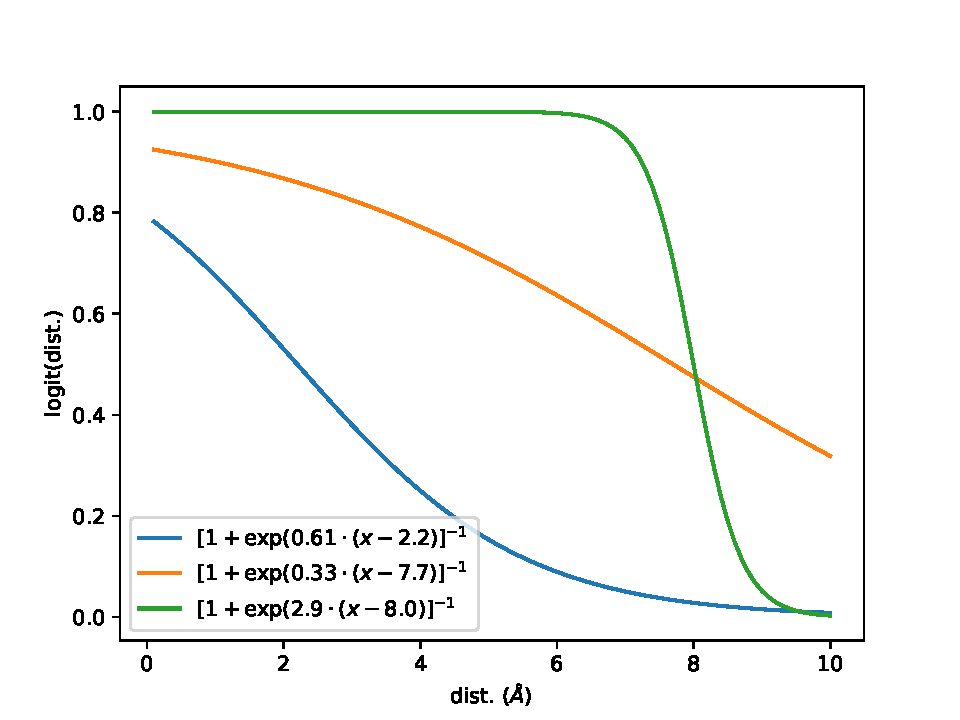
\includegraphics[height=0.25\textheight]{SI_figures/transforms.pdf}
    \caption{\textsc{Logistic transforms in select models.} The horizontal axis is the contact distance in \si{\angstrom}, the vertical axis shows the logistic transform of that distance for BBA model 1 (blue), model 4 (orange) and model 5 (green). }
    \label{fig:transforms}
\end{figure}

\section{Detailed model summaries} 


\subsection{Chignolin model 1}
This model has the largest median $t_{2}$ after random sampling optimisation.

\begin{figure}[h]
    \centering
    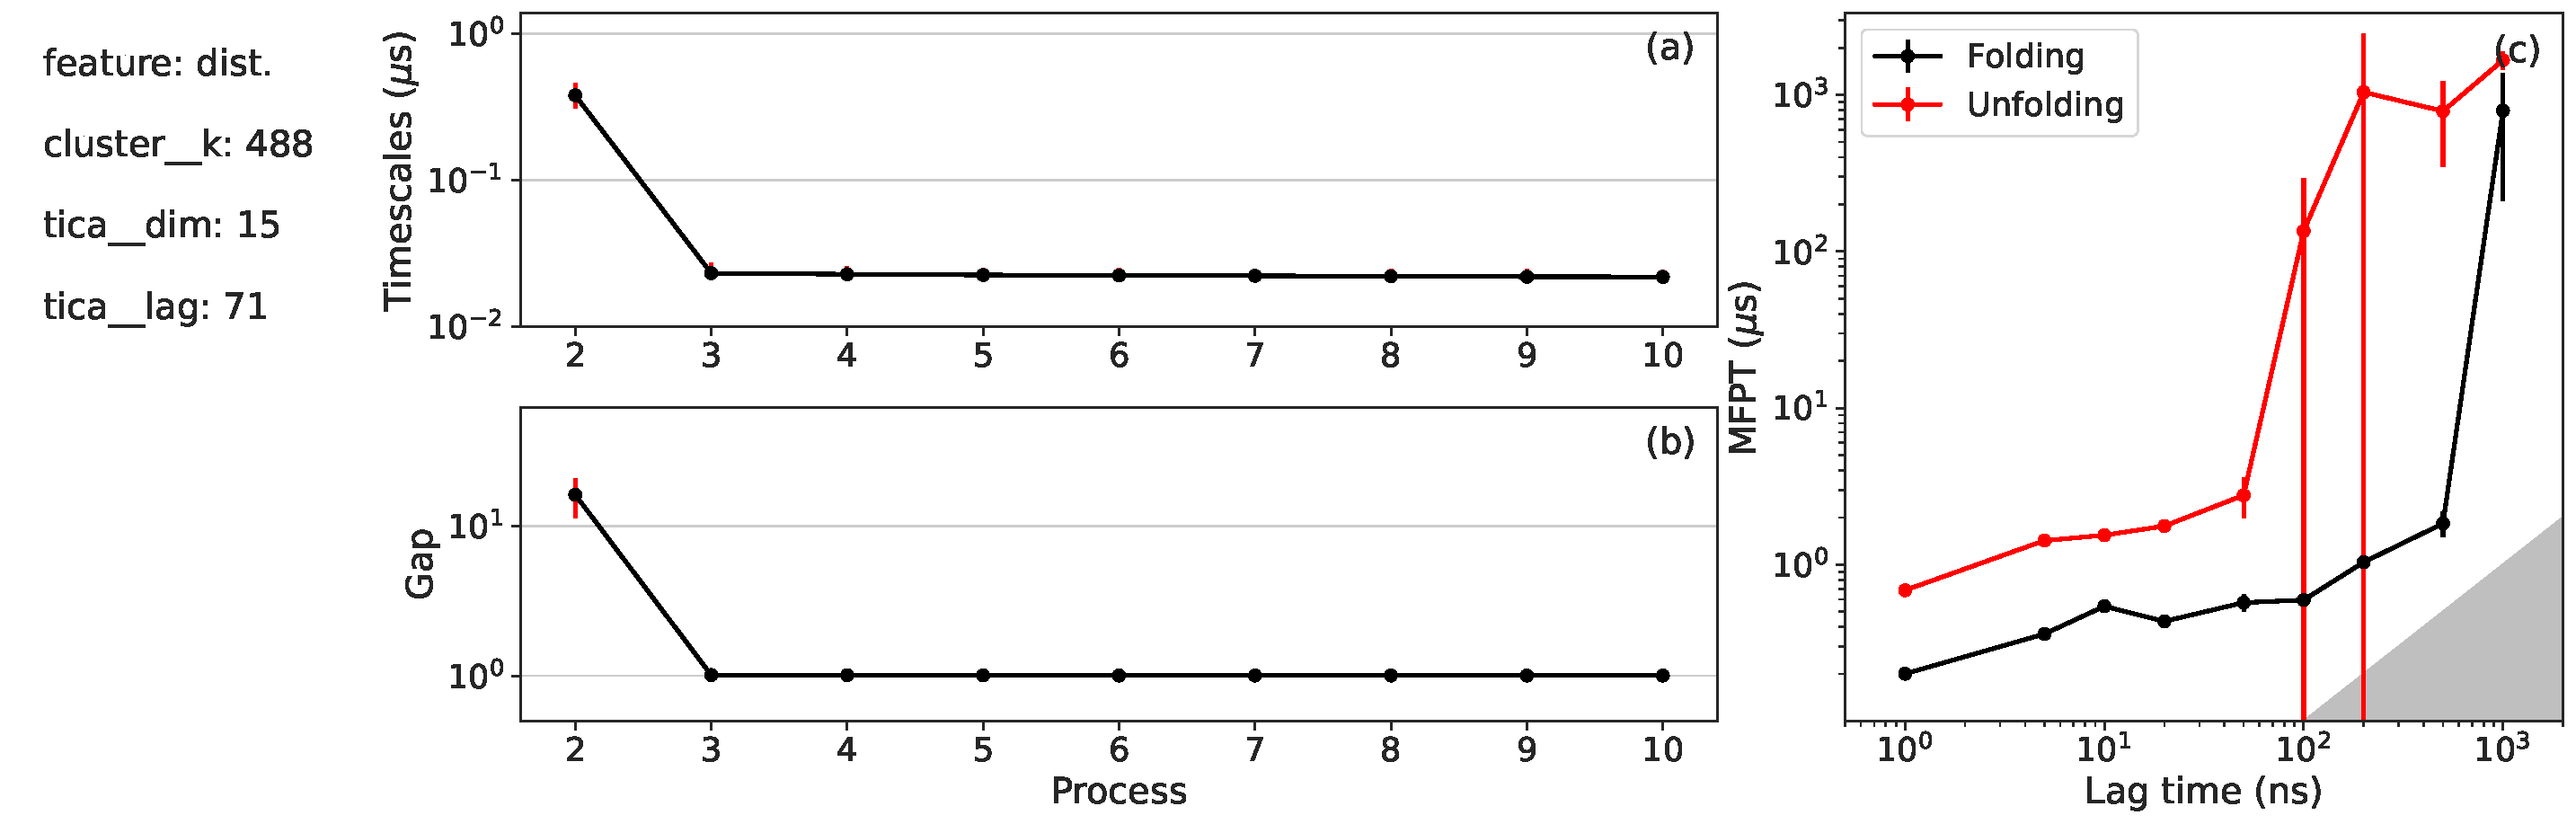
\includegraphics[width=\columnwidth]{SI_figures/CLN_52_SI-1.pdf}
    \caption{\textsc{Chignolin, model 1 timescales}.   Text inset shows the MSM hyperparameters; panel (a) shows the implied timescales for the first nine slow relaxation processes ($\tau=\SI{-1}{\nano\second}$); panel (b) shows the gap between successive successive timescales: the gap for process $i$ is defined as $t_{i}/t_{i+1}$ ($\tau=\SI{-1}{\nano\second}$); panel (c) shows the mean first passage time between the the unfolded and folded state as a function of $\tau$.}
    \label{si_fig:CLN_52_1}
\end{figure}

\begin{figure}[h]
    \centering
    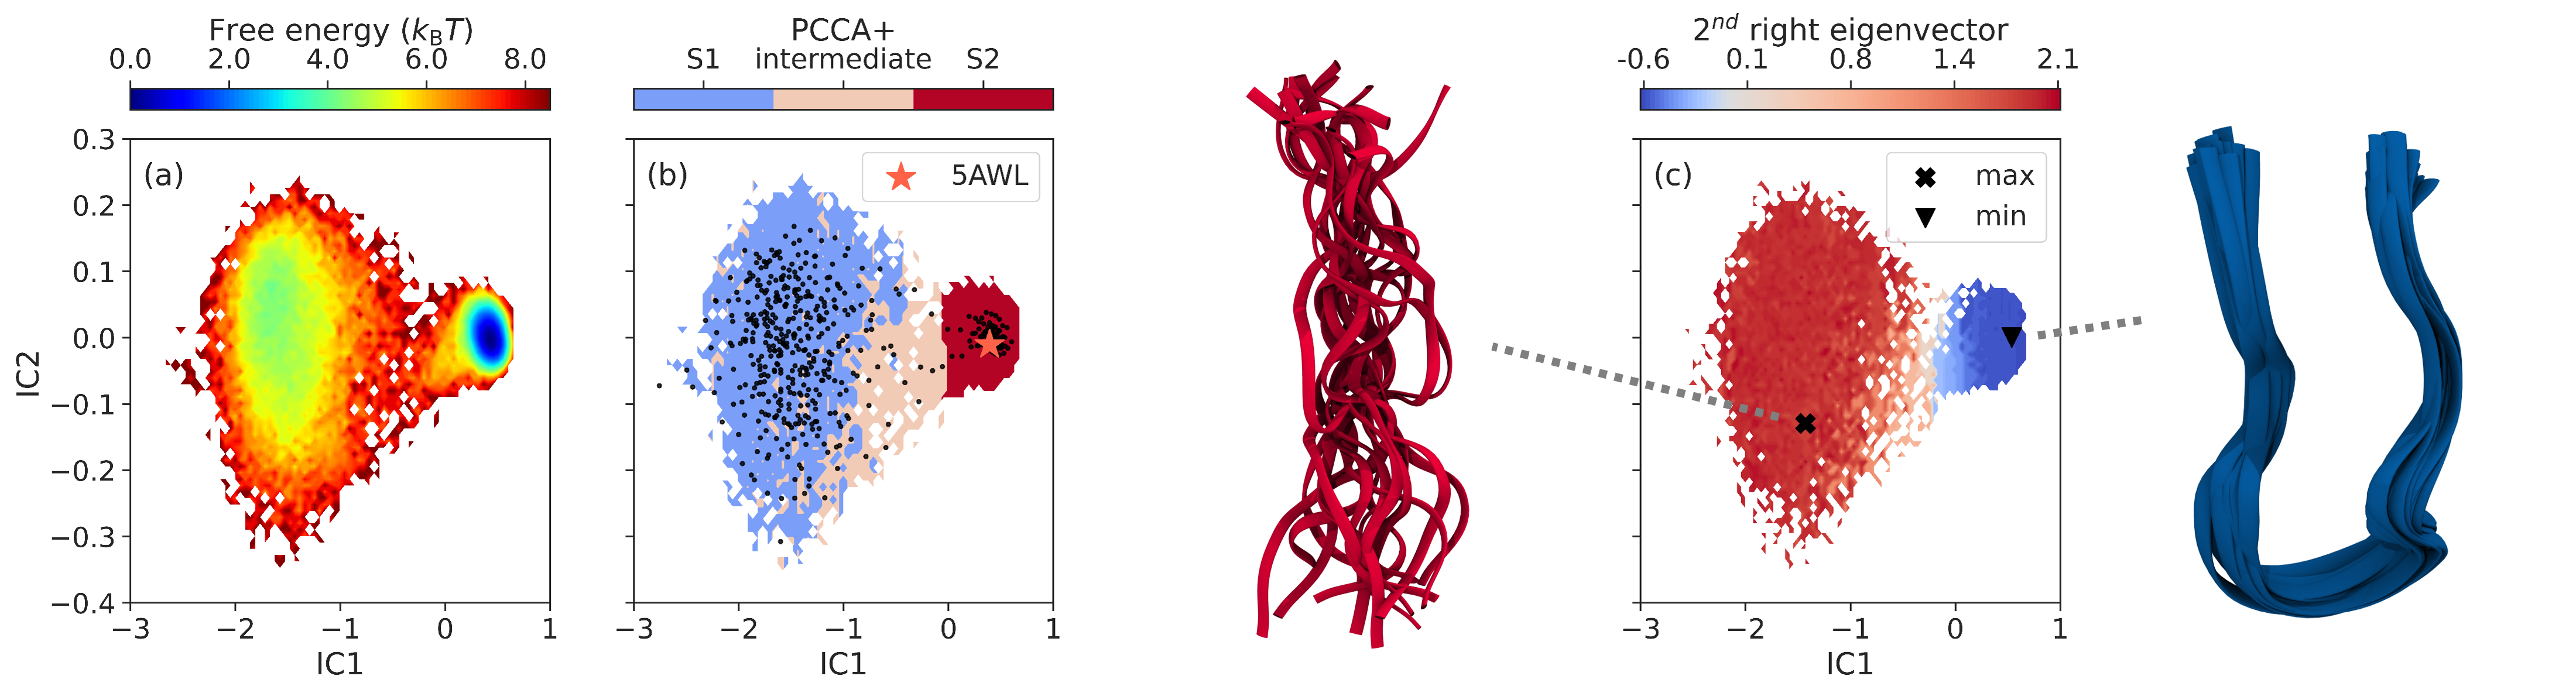
\includegraphics[width=\columnwidth]{SI_figures/CLN_52_SI-2.png}
    \caption{\textsc{Chignolin, model 1 free-energy surface}.  Each panel shows different quantities projected onto the first two TICA components (IC1, IC2).  Panel (a) shows the free energy surface; panel (b) shows the PCCA+ clustering into folded, unfolded and intermediate states with the crystal structure (PDB accession code 5AWL) marked with a star; panel (c) shows the 2nd right eigenvector (which corresponds to the slowest relaxation process) with an ensemble of structures corresponding to the extremes values of the eigenvector (`min', `max' marked with a triangle and cross respectively). }
    \label{si_fig:CLN_52_2}
\end{figure}


\begin{figure}[h]
    \centering
    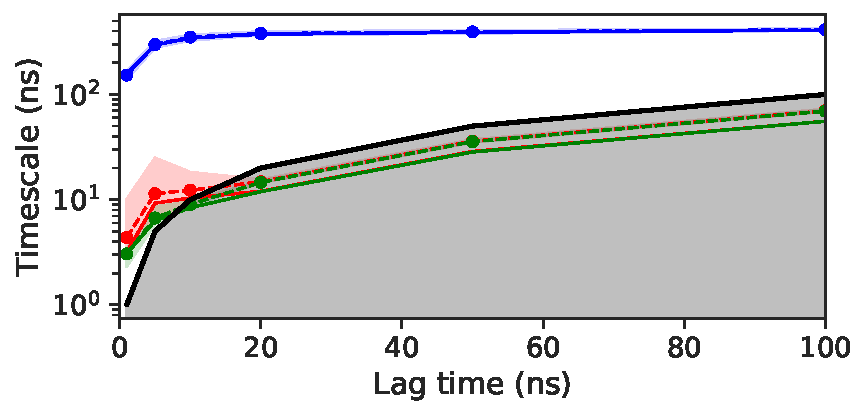
\includegraphics[height=0.15\textheight]{SI_figures/CLN_52_its.pdf}
    \caption{\textsc{Chignolin, model 1 validation}. The implied timescales plotted as a function of the lag-time. Blue, red, and green lines correspond to the slowest, second slowest, and third slowest process respectively. The solid lines correspond to the timescales from the maximum likelihood MSM. The dashed lines correspond to the mean of Bayesian MSMs. The coloured regions refer to the 0.95 confidence interval. The shaded region shows when the Markov lag time becomes equal to or longer than the implied timescale.}
    \label{si_fig:CLN_52_3}
\end{figure}

\FloatBarrier
\clearpage

\subsection{Chignolin model 2}

This model has the largest median $t_{2}$ using the logistic distance feature from random sampling.

\begin{figure}[h]
    \centering
    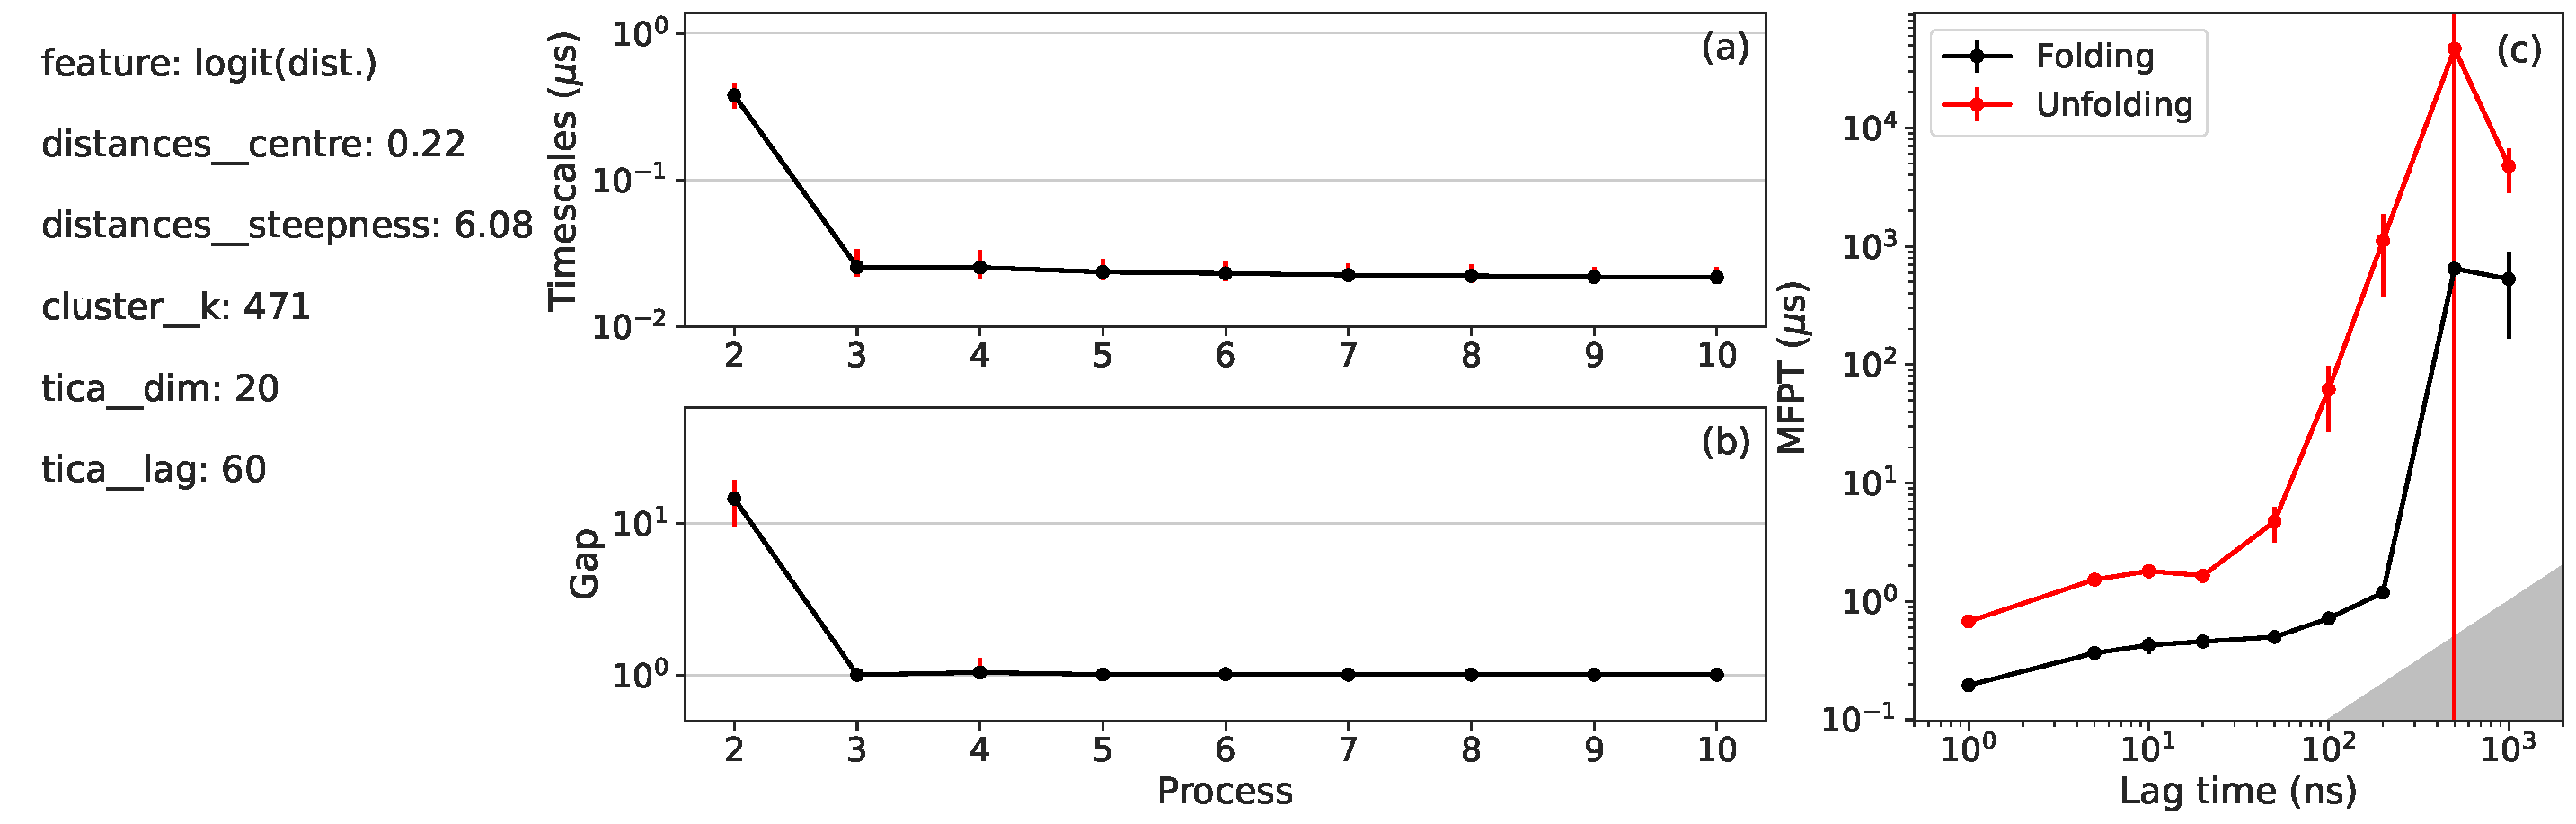
\includegraphics[width=\columnwidth]{SI_figures/CLN_23_SI1.pdf}
    \caption{\textsc{Chignolin,  model 2 timescales}.  See the caption for figure \ref{si_fig:CLN_52_1}. }
    \label{si_fig:CLN_24_1}
\end{figure}

\begin{figure}[h]
    \centering
    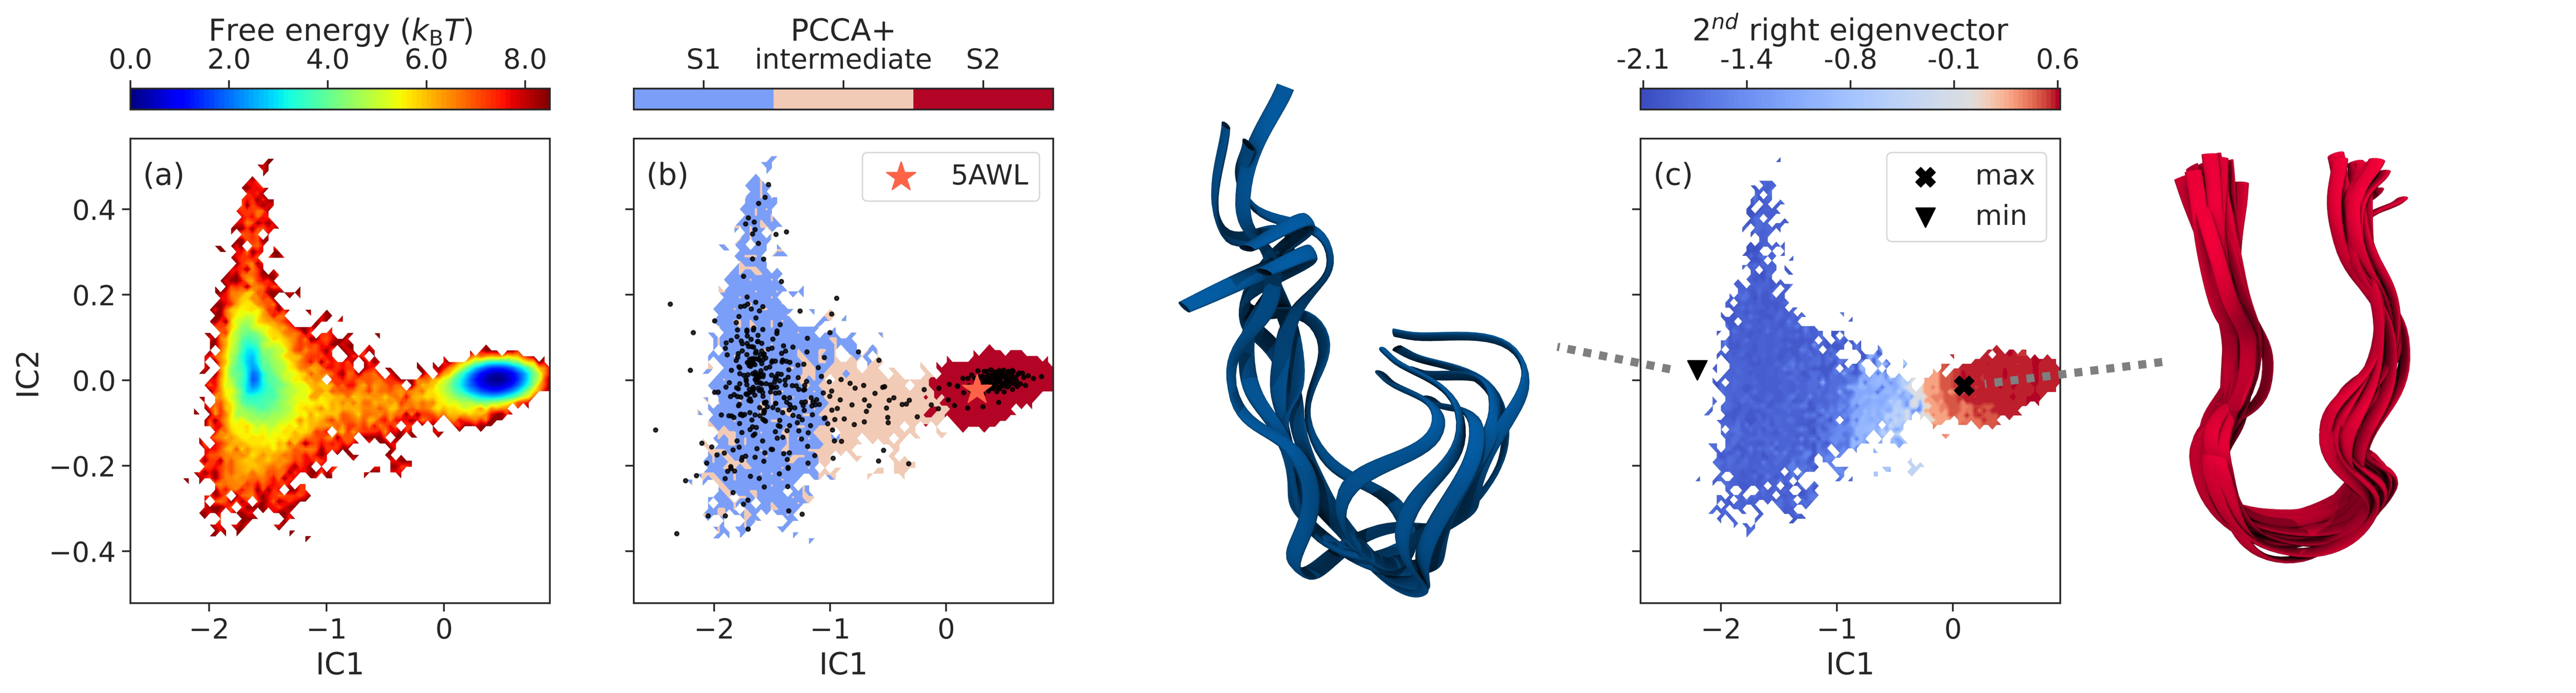
\includegraphics[width=\columnwidth]{SI_figures/CLN_23_SI2.png}
    \caption{\textsc{Chignolin,  model 2 free energy surface}. See the caption for figure \ref{si_fig:CLN_52_2}.}
    \label{si_fig:CLN_24_2}
\end{figure}

\begin{figure}[h]
    \centering
    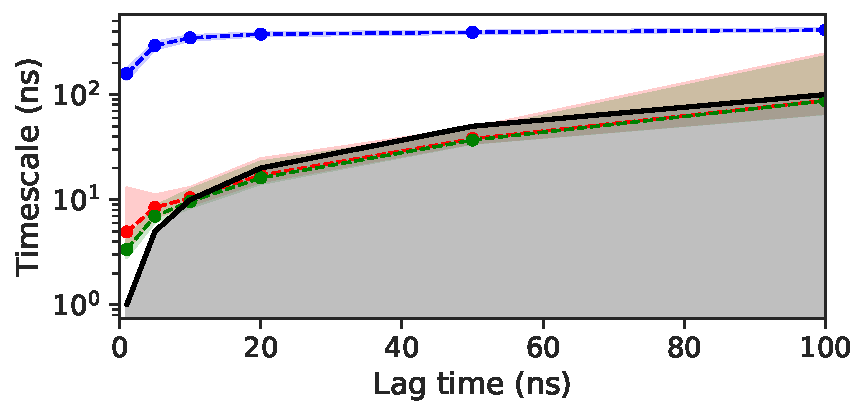
\includegraphics[height=0.15\textheight]{SI_figures/CLN_23_its.pdf}
    \caption{\textsc{Chignolin, model 2 validation}. See the caption for figure \ref{si_fig:CLN_52_3}.}
    \label{si_fig:CLN_24_3}
\end{figure}

\FloatBarrier
\clearpage

\subsection{Chignolin model 3}

This model has the largest median $t_{2}$ after Bayesian optimisation of $t_{2}$.

\begin{figure}[h]
    \centering
    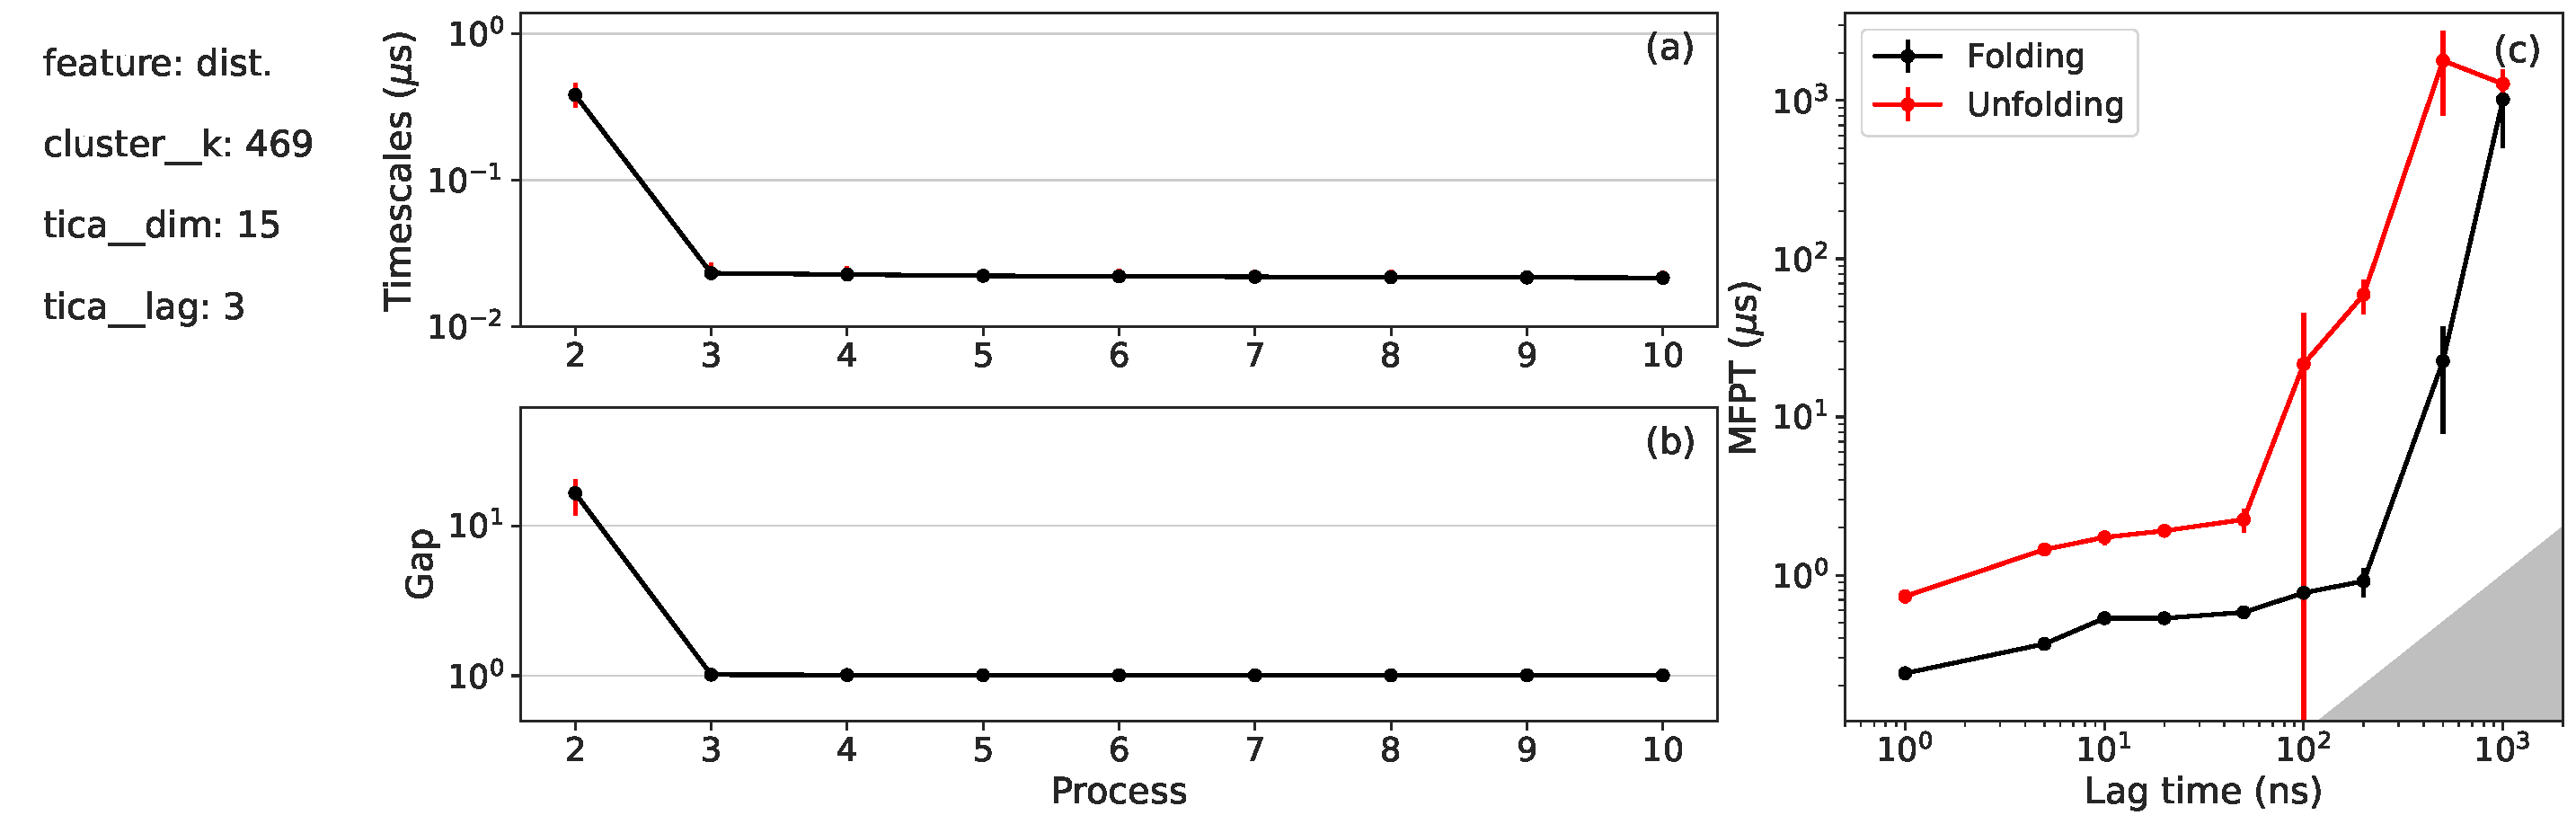
\includegraphics[width=\columnwidth]{SI_figures/CLN_218_SI-1.pdf}
    \caption{\textsc{Chignolin,  model 3 timescales}.  See the caption for figure \ref{si_fig:CLN_52_1}. }
    \label{si_fig:CLN_218_1}
\end{figure}

\begin{figure}[h]
    \centering
    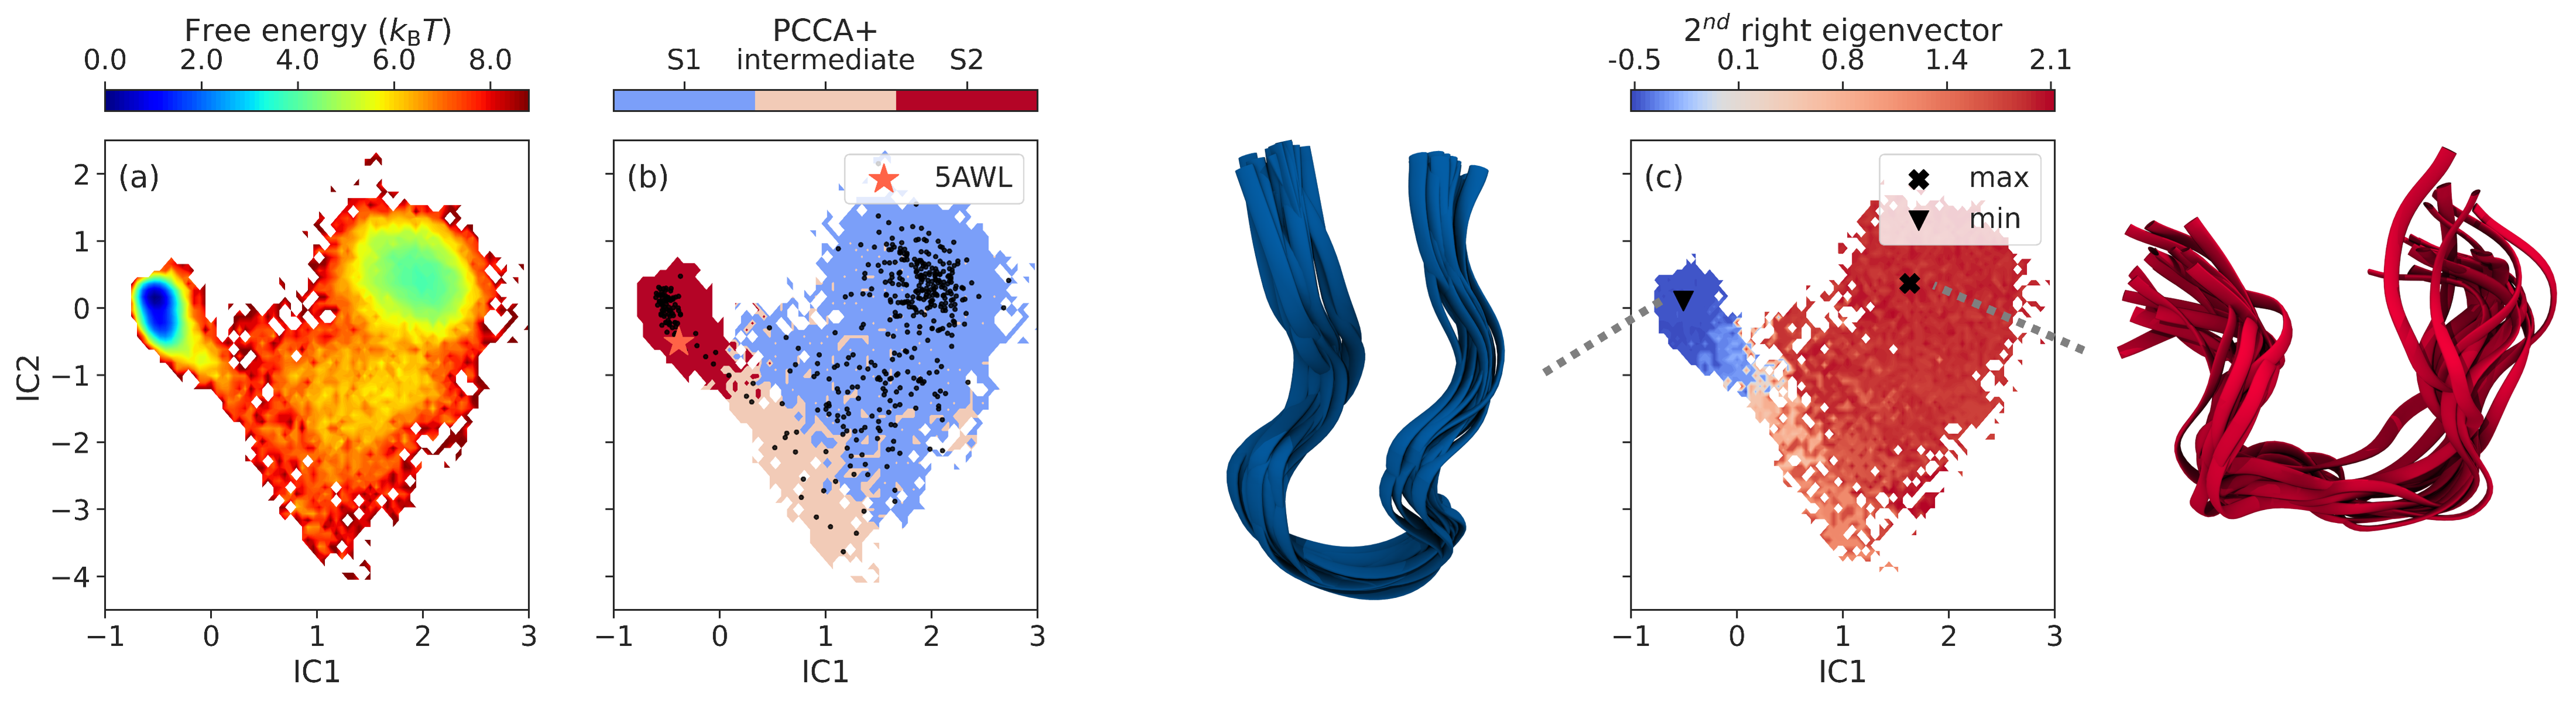
\includegraphics[width=\columnwidth]{SI_figures/CLN_218_SI-2.png}
    \caption{\textsc{Chignolin,  model 3 free energy surface}. See the caption for figure \ref{si_fig:CLN_52_2}.}
    \label{si_fig:CLN_218_2}
\end{figure}

\begin{figure}[h]
    \centering
    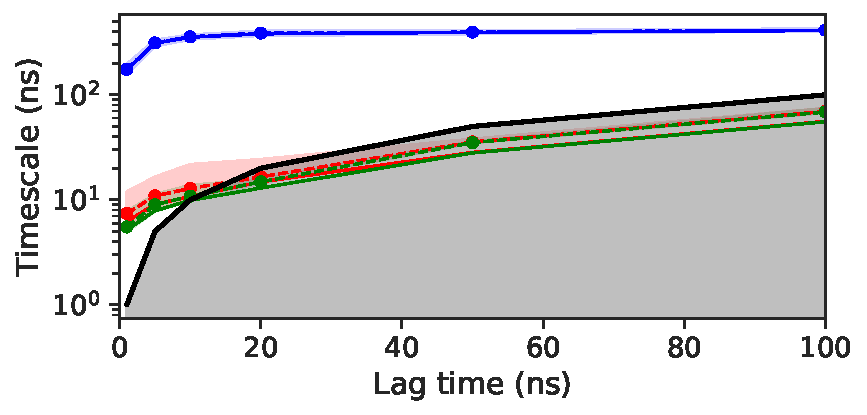
\includegraphics[height=0.15\textheight]{SI_figures/CLN_218_its.pdf}
    \caption{\textsc{Chignolin, model 3 validation}. See the caption for figure \ref{si_fig:CLN_52_3}.}
    \label{si_fig:CLN_218_3}
\end{figure}

\subsection{Chignolin model 4}

This model has the largest median $t_{2}$ after Bayesian optimisation of $\mathrm{VAMP2}_{eq}(2)$ and $\mathrm{VAMP2}_{eq}(2)/\mathrm{VAMP2}_{eq}(3)$.

\begin{figure}[h]
    \centering
    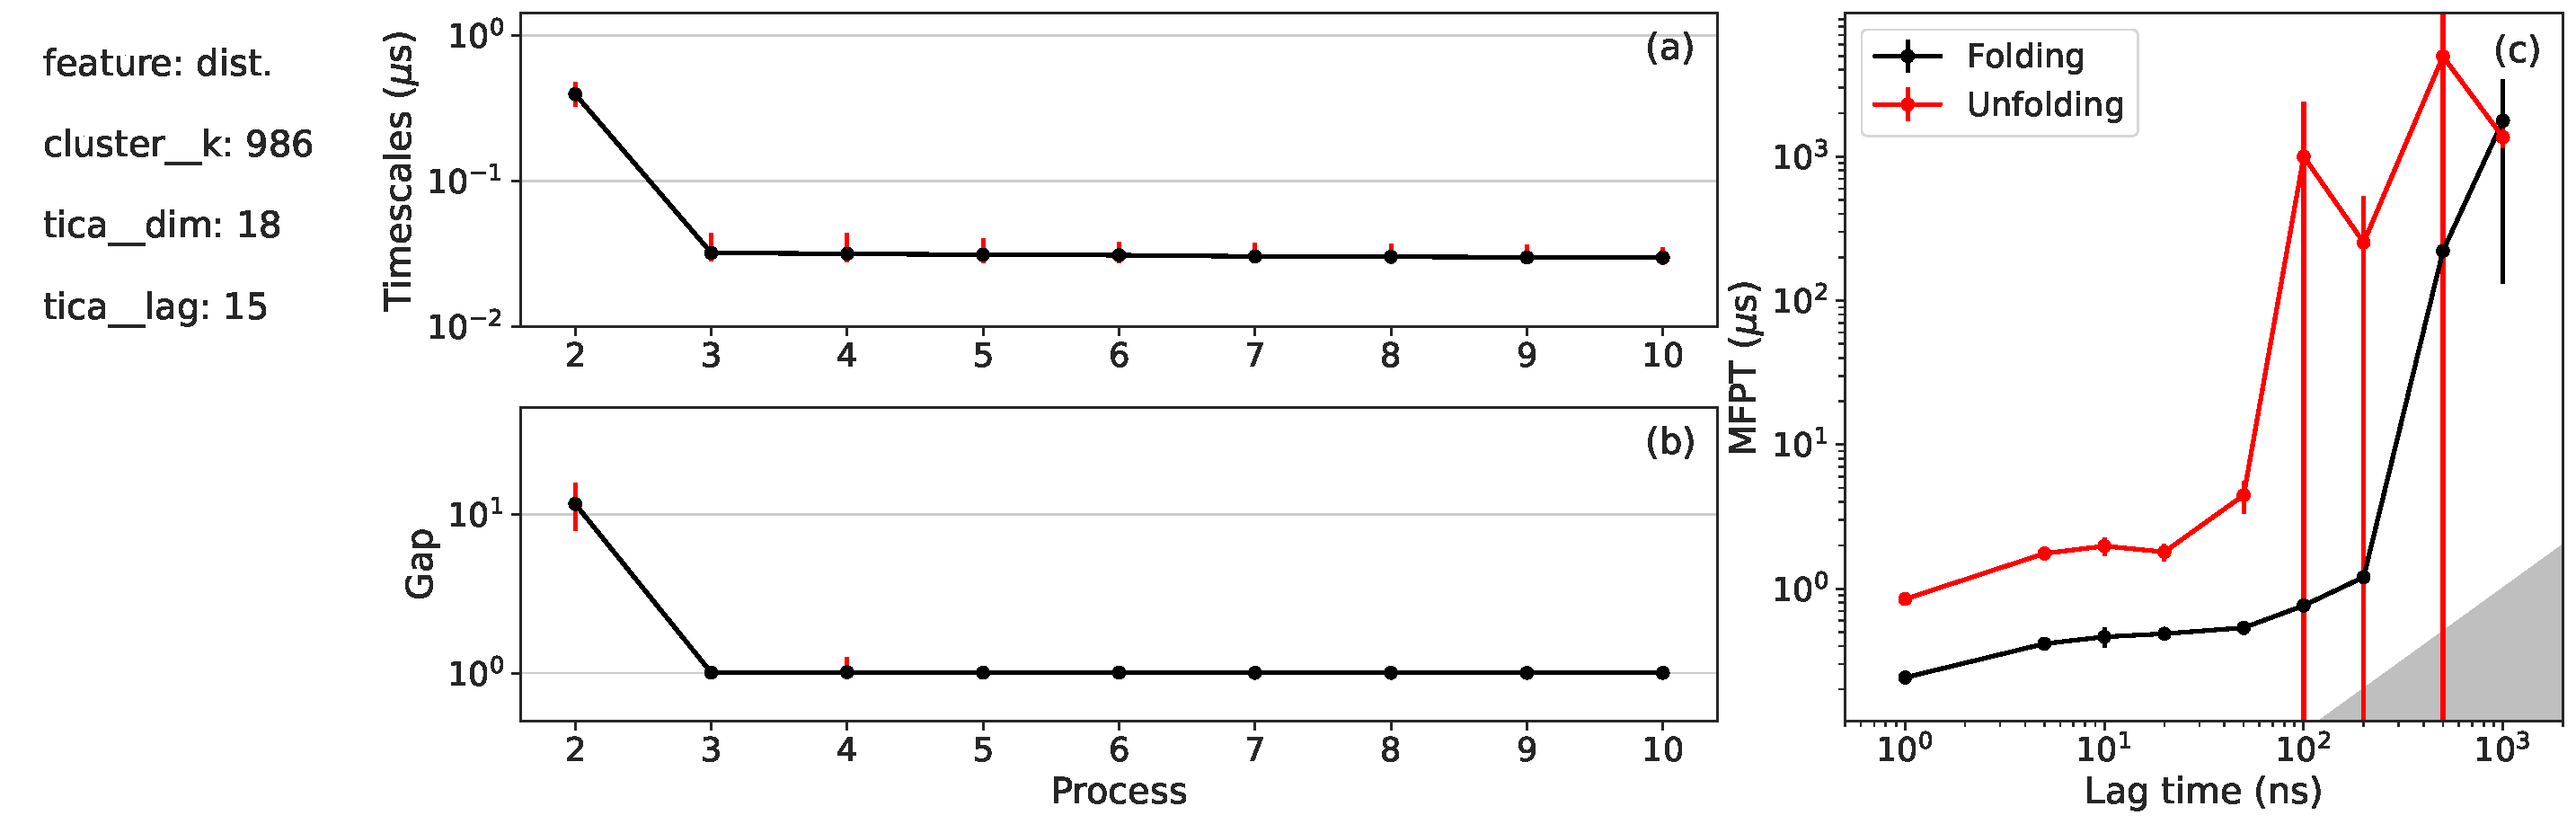
\includegraphics[width=\columnwidth]{SI_figures/CLN_93_SI1.pdf}
    \caption{\textsc{Chignolin,  model 4 timescales}.  See the caption for figure \ref{si_fig:CLN_52_1}. }
    \label{si_fig:CLN_93_1}
\end{figure}

\begin{figure}[h]
    \centering
    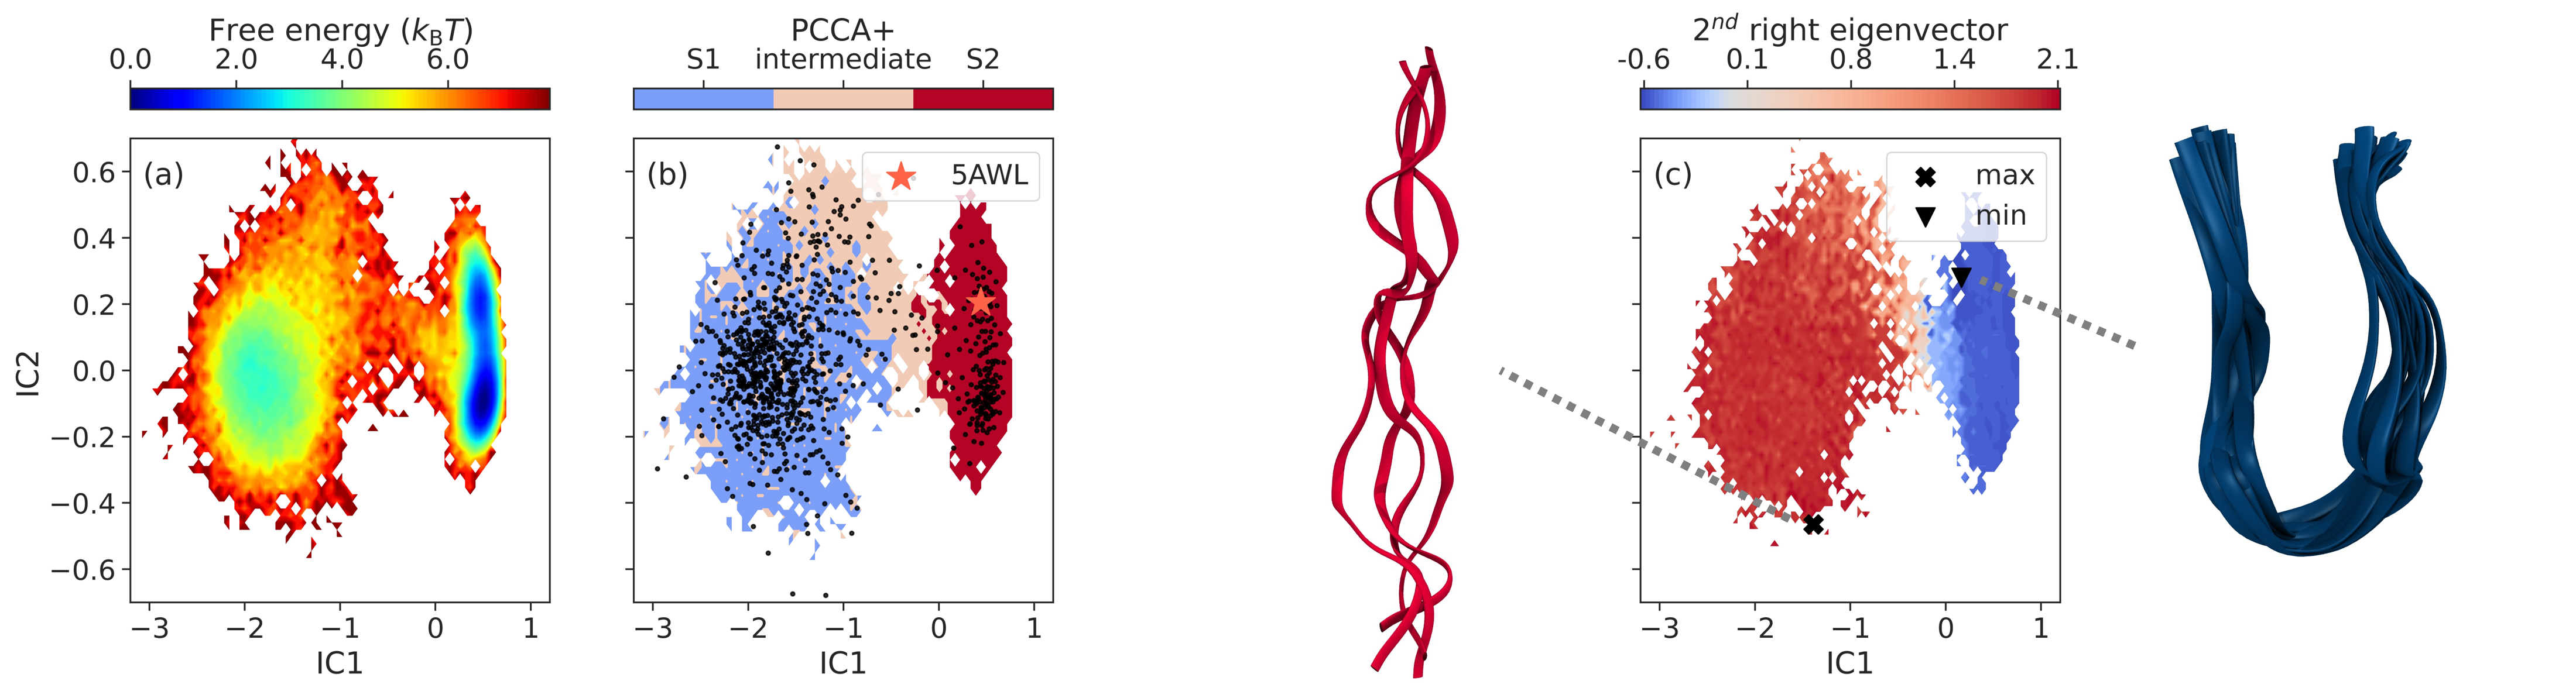
\includegraphics[width=\columnwidth]{SI_figures/CLN_93_SI2.png}
    \caption{\textsc{Chignolin,  model 4 free energy surface}. See the caption for figure \ref{si_fig:CLN_52_2}.}
    \label{si_fig:CLN_93_2}
\end{figure}

\begin{figure}[h]
    \centering
    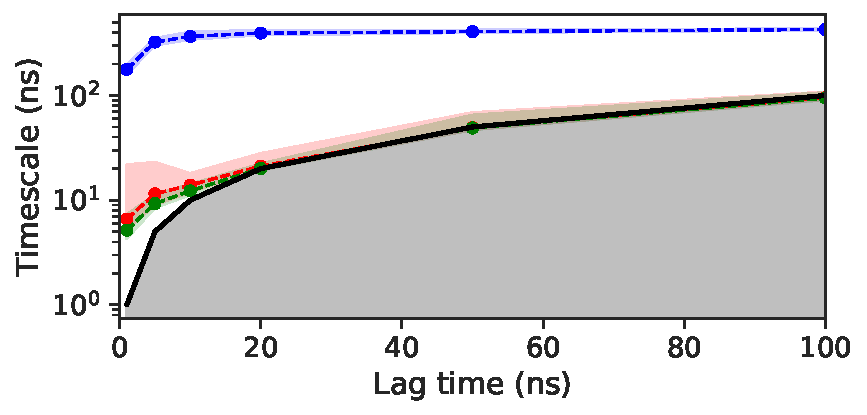
\includegraphics[height=0.15\textheight]{SI_figures/CLN_93_its.pdf}
    \caption{\textsc{Chignolin, model 4 validation}. See the caption for figure \ref{si_fig:CLN_52_3}.}
    \label{si_fig:CLN_93_3}
\end{figure}

\FloatBarrier
\clearpage


\subsection{BBA model 1}

This model has the largest median $t_{2}$ after random sampling.

\begin{figure}[h]
    \centering
    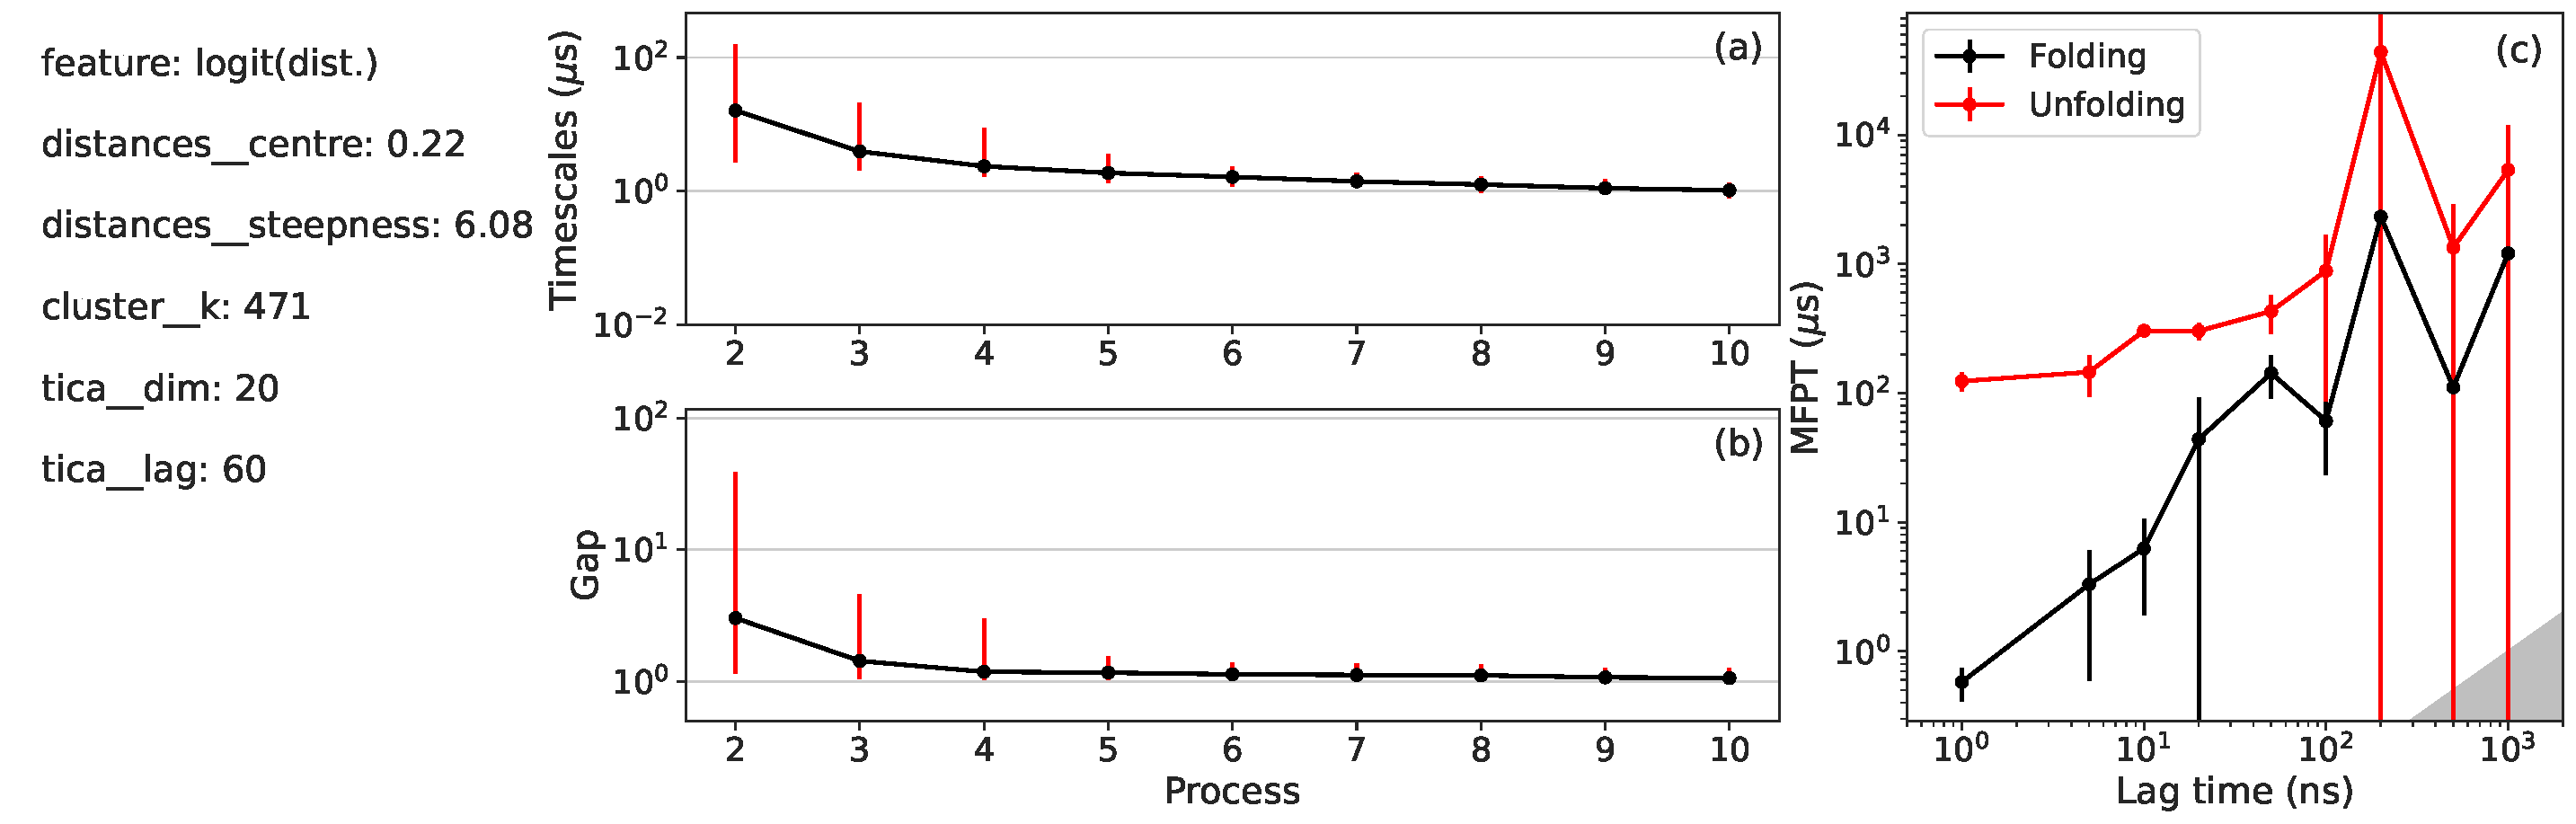
\includegraphics[width=\columnwidth]{SI_figures/BBA_24_SI-1.pdf}
    \caption{\textsc{BBA,  model 1 timescales.} Text inset shows the MSM hyperparameters; panel (a) shows the implied timescales for the first nine slow relaxation processes ($\tau=\SI{41}{\nano\second}$); panel (b) shows the gap between successive successive timescales: the gap for process $i$ is defined as $t_{i}/t_{i+1}$ ($\tau=\SI{41}{\nano\second}$); panel (c) shows the mean first passage time between the the unfolded and folded state as a function of $\tau$.}
    \label{si_fig:BBA_24_1}
\end{figure}

\begin{figure}[h]
    \centering
    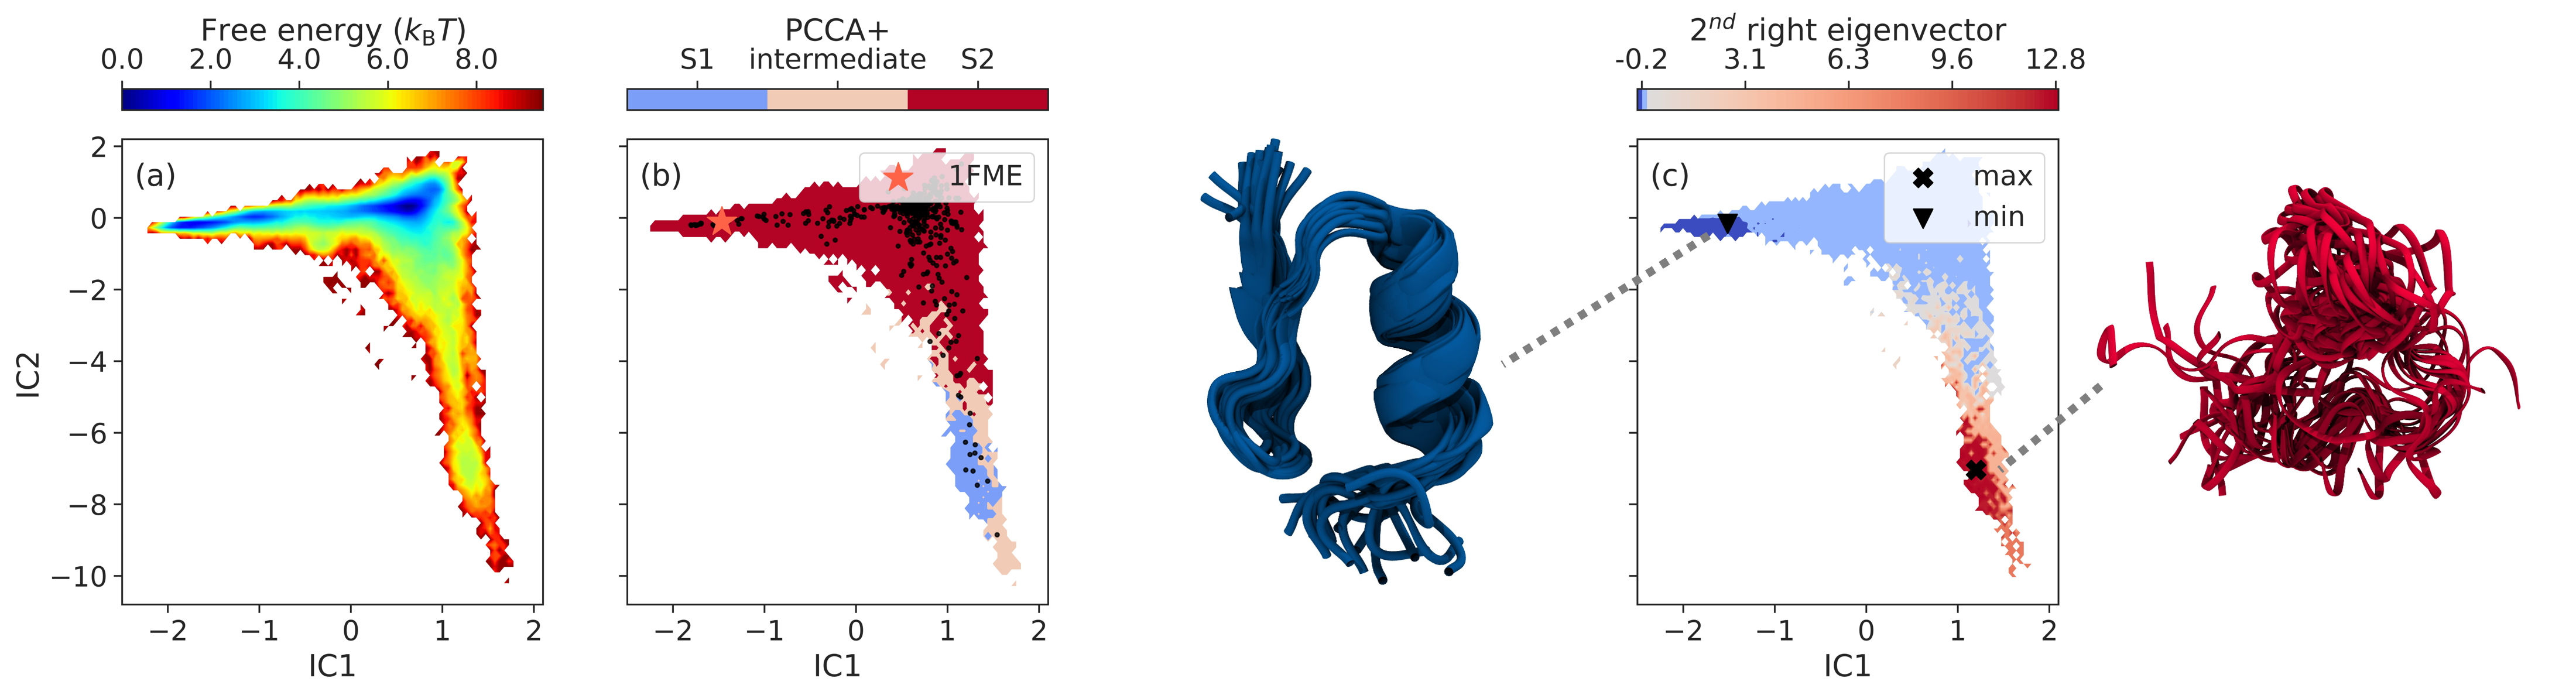
\includegraphics[width=\columnwidth]{SI_figures/BBA_24_SI-2.png}
    \caption{\textsc{BBA,  model 1 free energy surface}. Each panel shows different quantities projected onto the first two TICA components (IC1, IC2).  Panel (a) shows the free energy surface; panel (b) shows the PCCA+ clustering into folded, unfolded and intermediate states with the crystal structure (PDB accession code 1FME) marked with a star; panel (c) shows the 2nd right eigenvector (which corresponds to the slowest relaxation process) with an ensemble of structures corresponding to the extremes values of the eigenvector (`min', `max' marked with a triangle and cross respectively). }
    \label{si_fig:BBA_24_2}
\end{figure}

\begin{figure}[h]
    \centering
    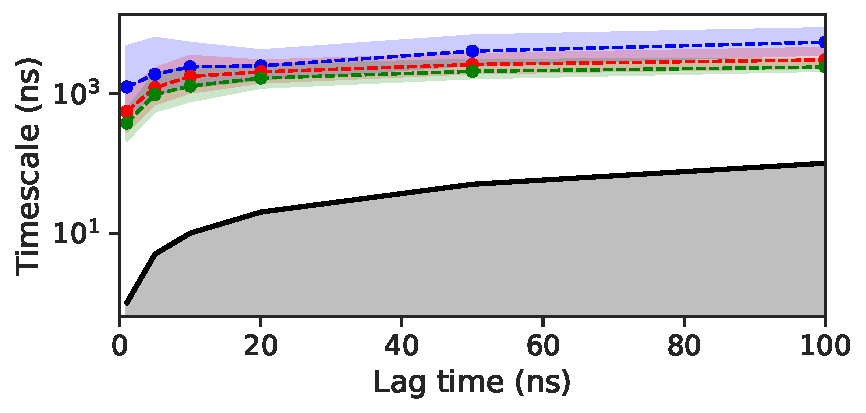
\includegraphics[height=0.15\textheight]{SI_figures/BBA_24_its.pdf}
    \caption{\textsc{BBA, model 1 validation}. The implied timescales plotted as a function of the lag-time. Blue, red, and green lines correspond to the slowest, second slowest, and third slowest process respectively. The solid lines correspond to the timescales from the maximum likelihood MSM. The dashed lines correspond to the mean of Bayesian MSMs. The coloured regions refer to the 0.95 confidence interval. The shaded region shows when the Markov lag time becomes equal to or longer than the implied timescale.}
    \label{si_fig:BBA_24_3}
\end{figure}

\FloatBarrier
\clearpage


\subsection{BBA model 2}

This model has the second largest median $t_{2}$ after random sampling. 

\begin{figure}[h]
    \centering
    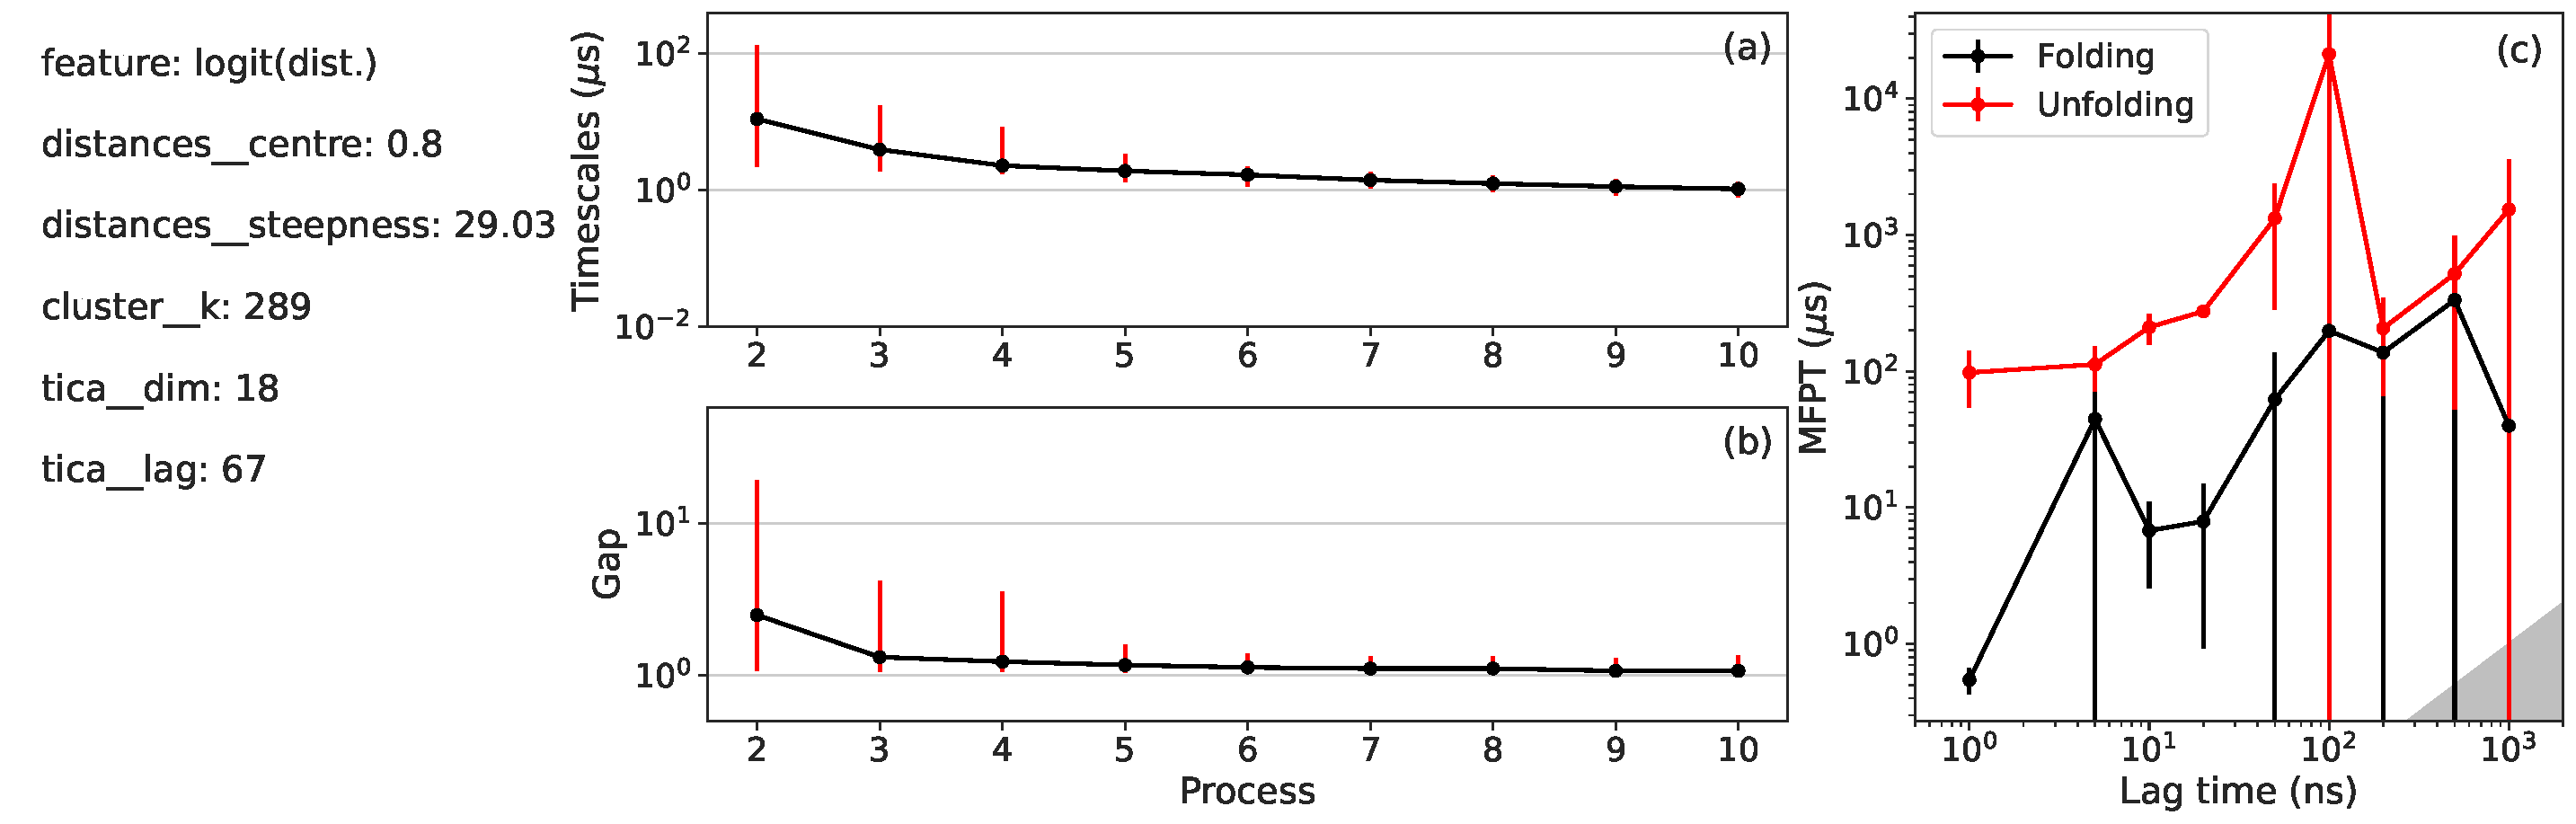
\includegraphics[width=\columnwidth]{SI_figures/BBA_124_SI-1.pdf}
    \caption{\textsc{BBA, model 2 timescales}. See the caption for figure \ref{si_fig:BBA_24_1}.}
    \label{si_fig:BBA_000_1}
\end{figure}

\begin{figure}[h]
    \centering
    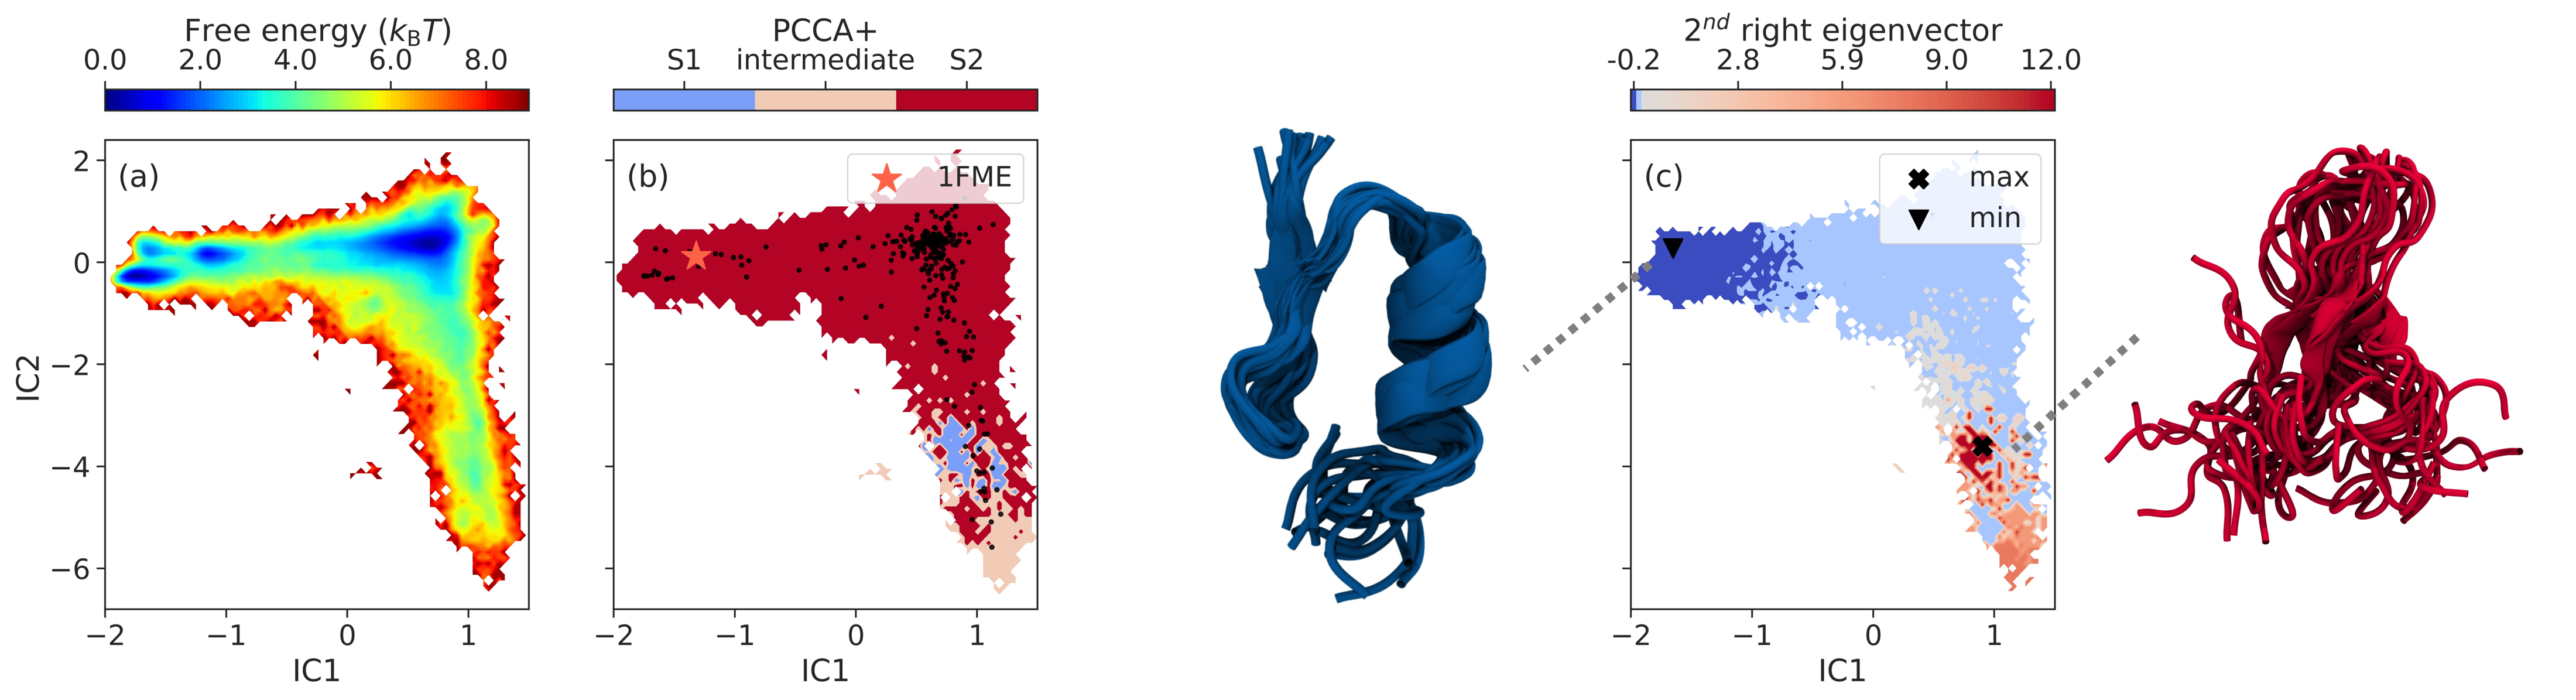
\includegraphics[width=\columnwidth]{SI_figures/BBA_124_SI-2.png}
    \caption{\textsc{BBA,  model 2 free energy surface}. See the caption for figure \ref{si_fig:BBA_24_2}.}
    \label{si_fig:BBA_000_2}
\end{figure}

\begin{figure}[h]
    \centering
    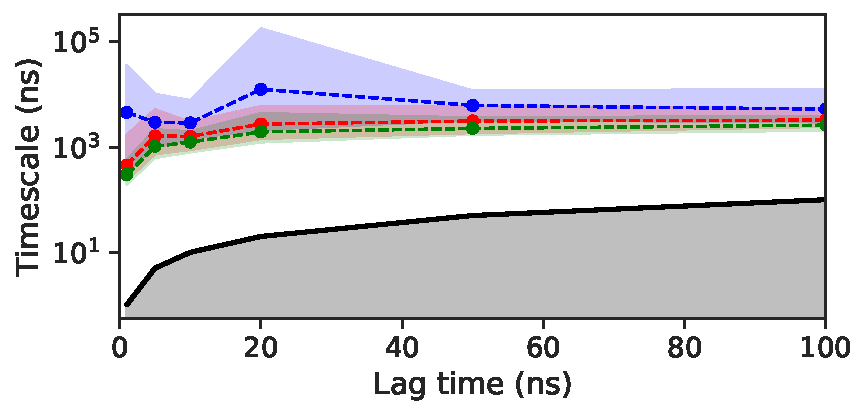
\includegraphics[height=0.15\textheight]{SI_figures/BBA_124_its.pdf}
    \caption{\textsc{BBA, model 2 validation}. See the caption for  figure \ref{si_fig:BBA_24_3}.}
    \label{si_fig:BBA_000_3}
\end{figure}

\FloatBarrier
\clearpage


\subsection{BBA model 3}

This model has the largest median $t_{2}$ using the distance feature after random sampling. 

\begin{figure}[h]
    \centering
    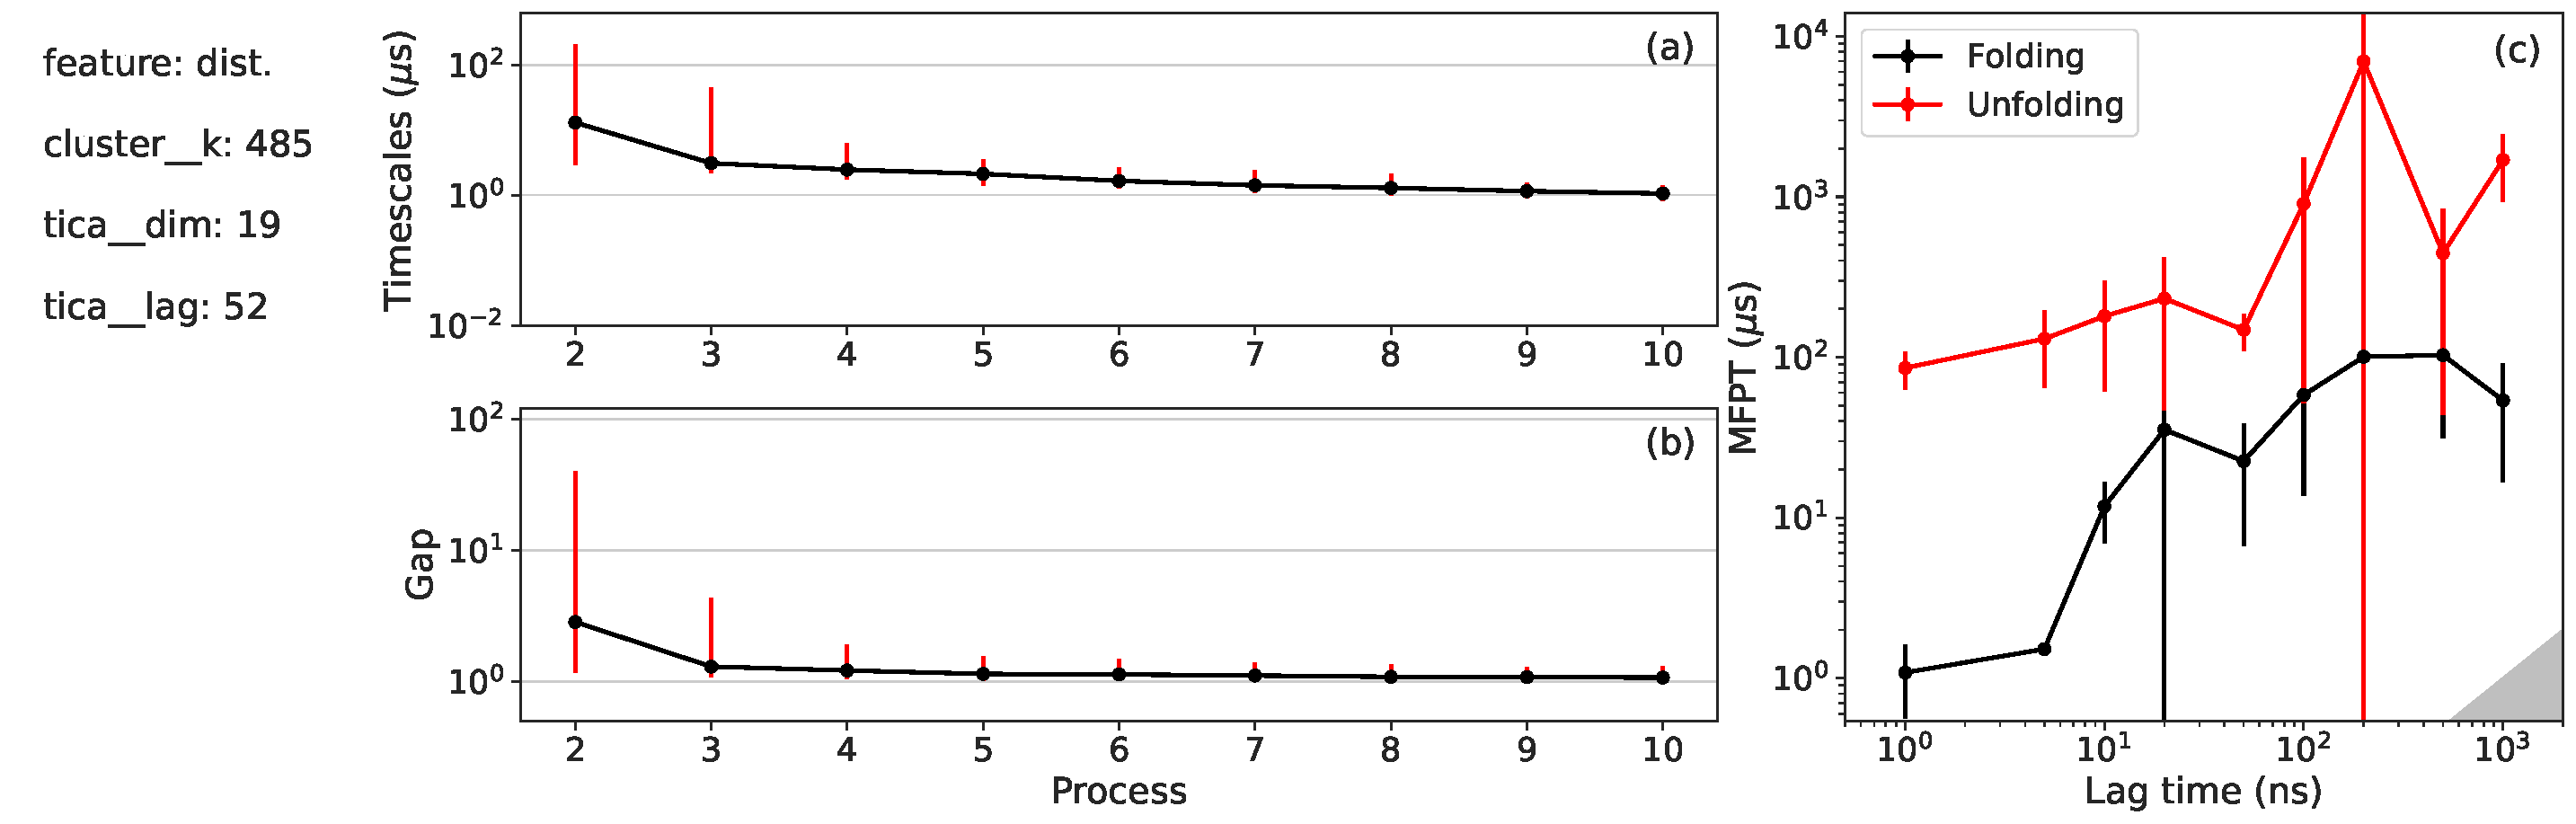
\includegraphics[width=\columnwidth]{SI_figures/BBA_58_SI-1.pdf}
    \caption{\textsc{BBA, model 3 timescales}. See the caption for figure \ref{si_fig:BBA_24_1}. }
    \label{si_fig:BBA_58_1}
\end{figure}

\begin{figure}[h]
    \centering
    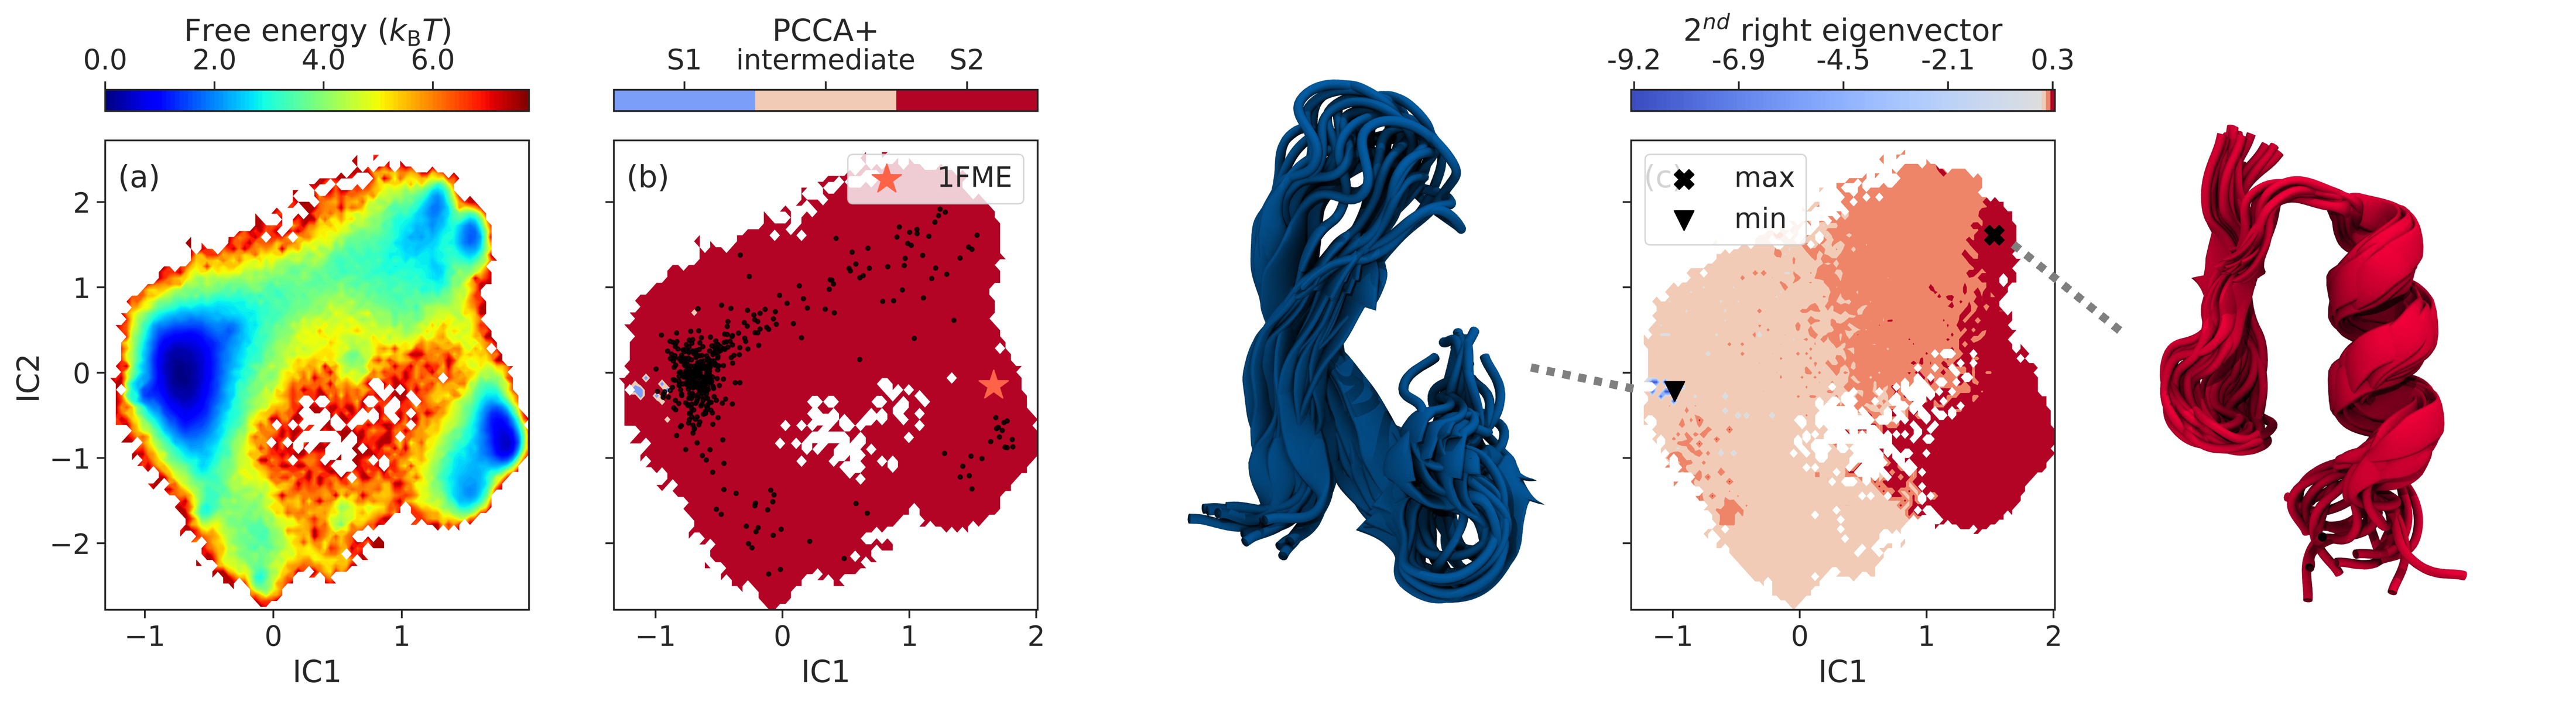
\includegraphics[width=\columnwidth]{SI_figures/BBA_58_SI-2.png}
    \caption{\textsc{BBA, model 3 free energy surface}. See the caption for figure \ref{si_fig:BBA_24_2}. }
    \label{si_fig:BBA_58_2}
\end{figure}

\begin{figure}[h]
    \centering
    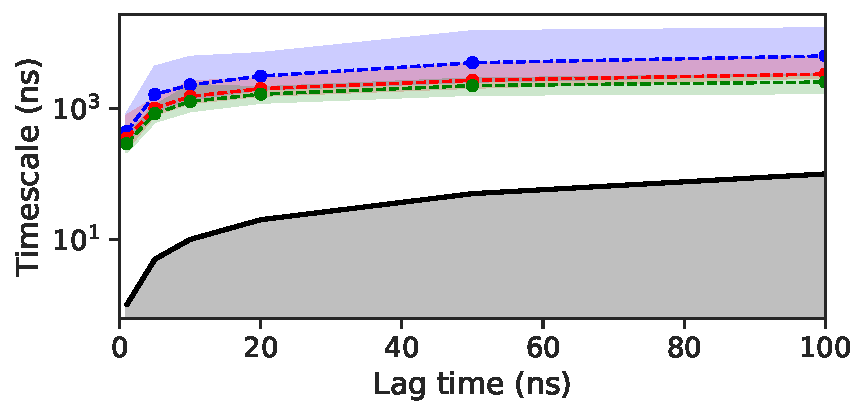
\includegraphics[height=0.15\textheight]{SI_figures/BBA_58_its.pdf}
    \caption{\textsc{BBA, model 3 validation}.  See the caption for figure \ref{si_fig:BBA_24_3}.}
    \label{si_fig:BBA_58_3}
\end{figure}

\FloatBarrier
\clearpage


\subsection{BBA model 4}

This model has the largest median $t_{2}$ using the dihedral feature after random sampling.

\begin{figure}[h]
    \centering
    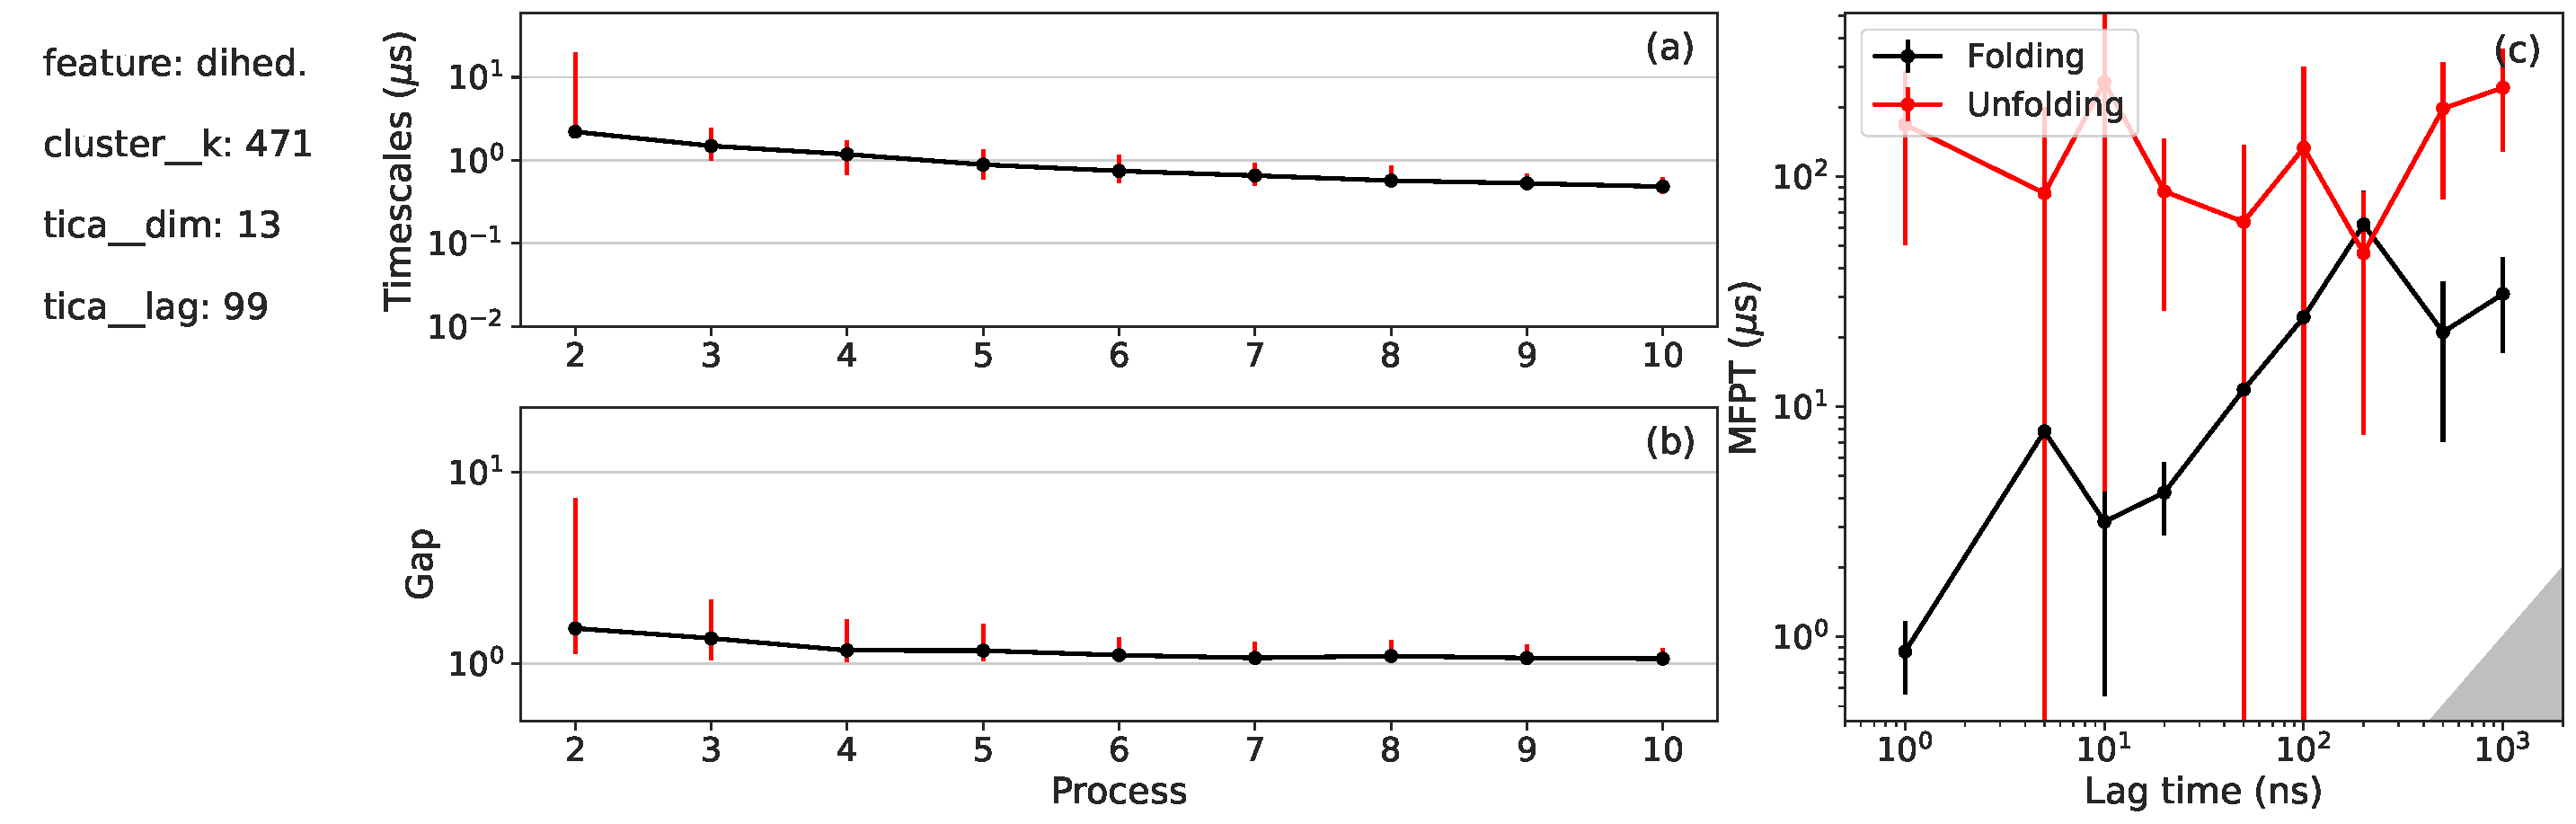
\includegraphics[width=\columnwidth]{SI_figures/BBA_6_SI-1.pdf}
    \caption{\textsc{BBA,  model 4 timescales}. See the caption for figure \ref{si_fig:BBA_24_1}.}
    \label{si_fig:BBA_6_1}
\end{figure}

\begin{figure}[h]
    \centering
    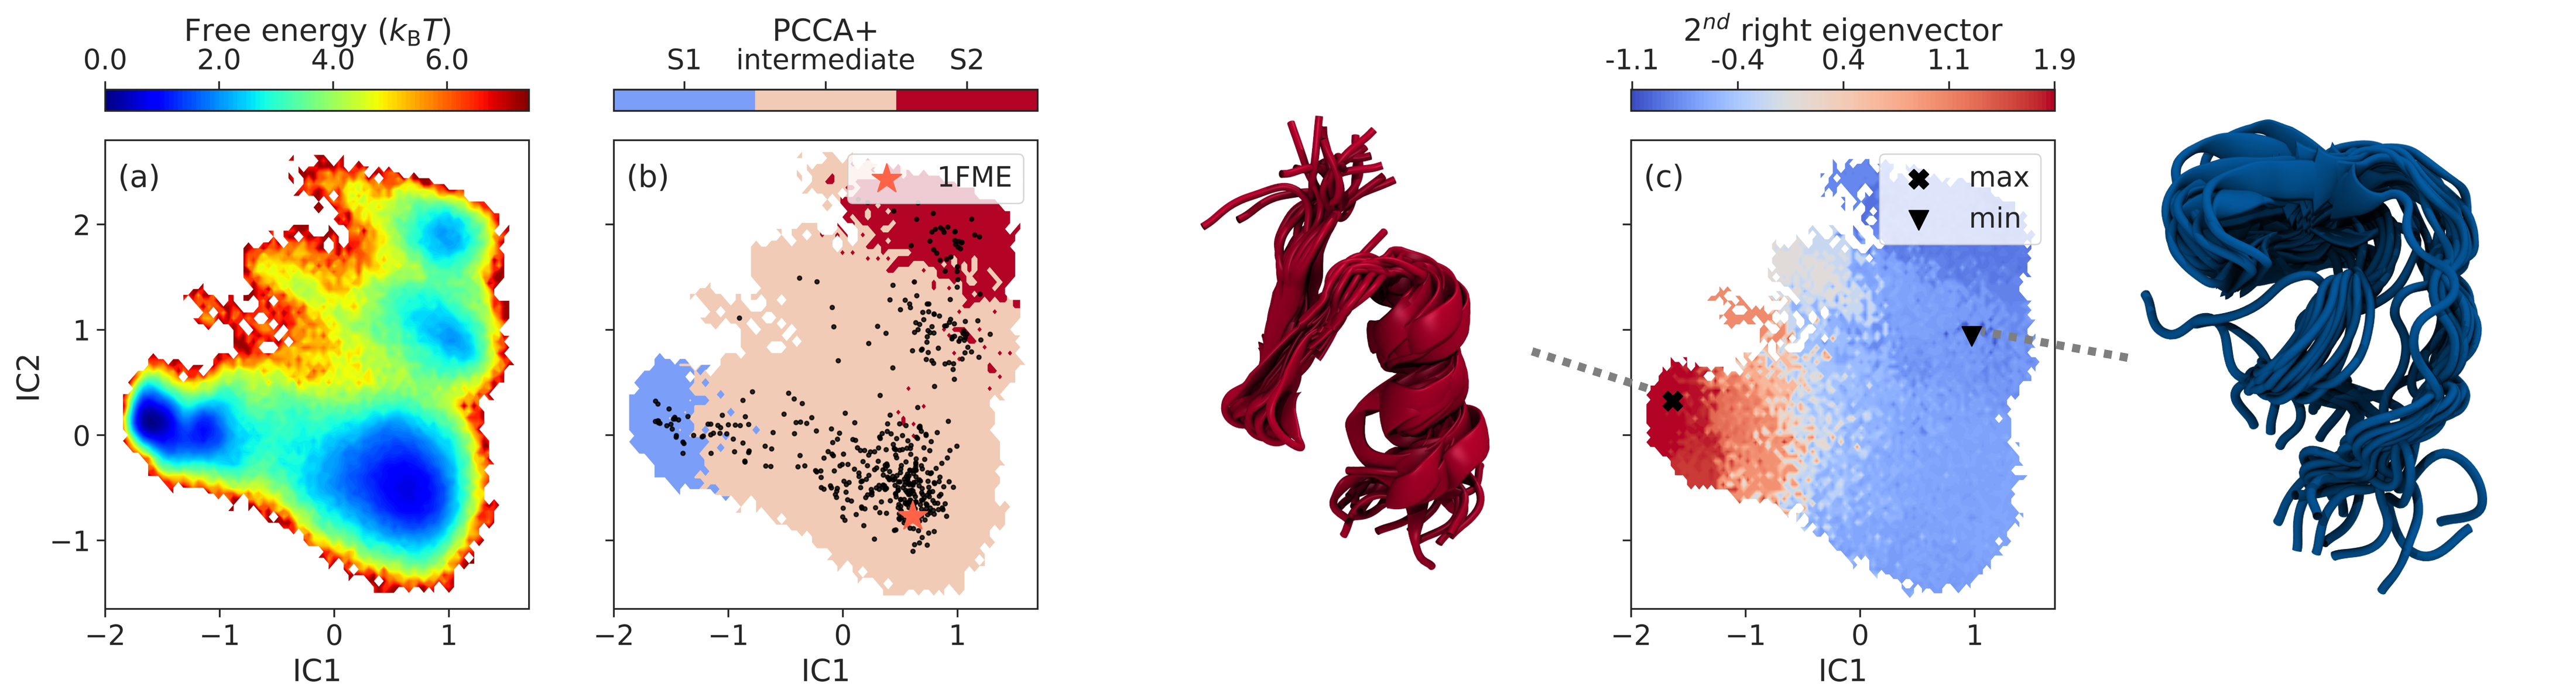
\includegraphics[width=\columnwidth]{SI_figures/BBA_6_SI-2.png}
    \caption{\textsc{BBA,  model 4 free energy surface}. See the caption for figure \ref{si_fig:BBA_24_2}.}
    \label{si_fig:BBA_6_2}
\end{figure}

\begin{figure}[h]
    \centering
    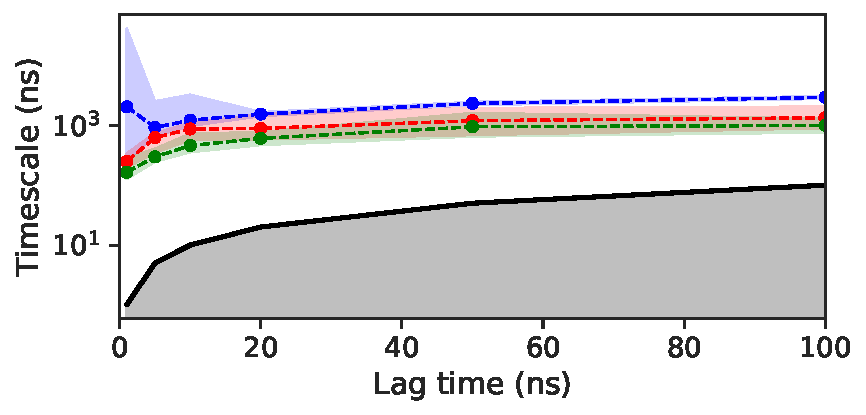
\includegraphics[height=0.15\textheight]{SI_figures/BBA_6_its.pdf}
    \caption{\textsc{BBA, model 4 validation}.  See the caption for figure \ref{si_fig:BBA_24_3}.}
    \label{si_fig:BBA_6_3}
\end{figure}

\FloatBarrier
\clearpage



\subsection{BBA model 5}

This model has the largest median $t_{2}$ after Bayesian optimisation of $t_2$.

\begin{figure}[h]
    \centering
    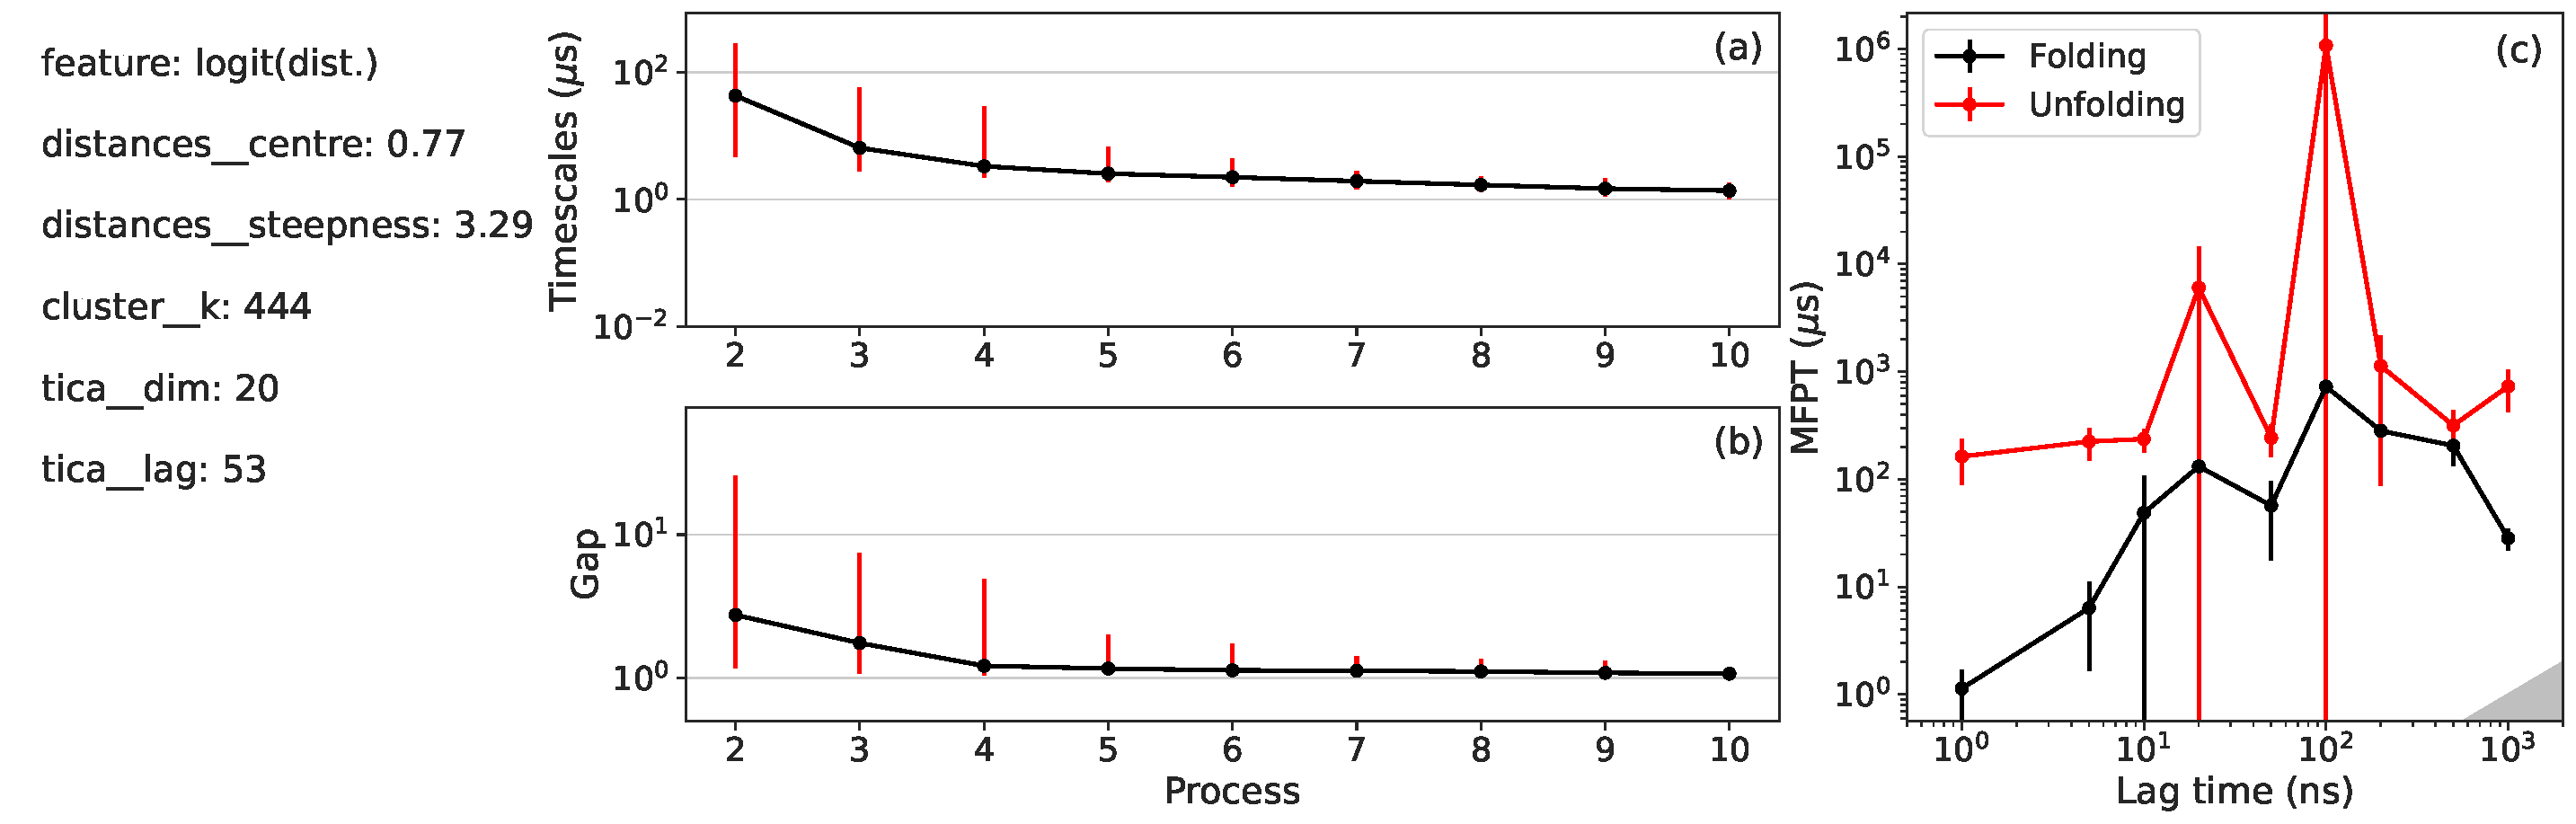
\includegraphics[width=\columnwidth]{SI_figures/BBA_227_SI-1.pdf}
    \caption{\textsc{BBA,  model 5 timescales}. See the caption for figure \ref{si_fig:BBA_24_1}.}
    \label{si_fig:BBA_227_1}
\end{figure}

\begin{figure}[h]
    \centering
    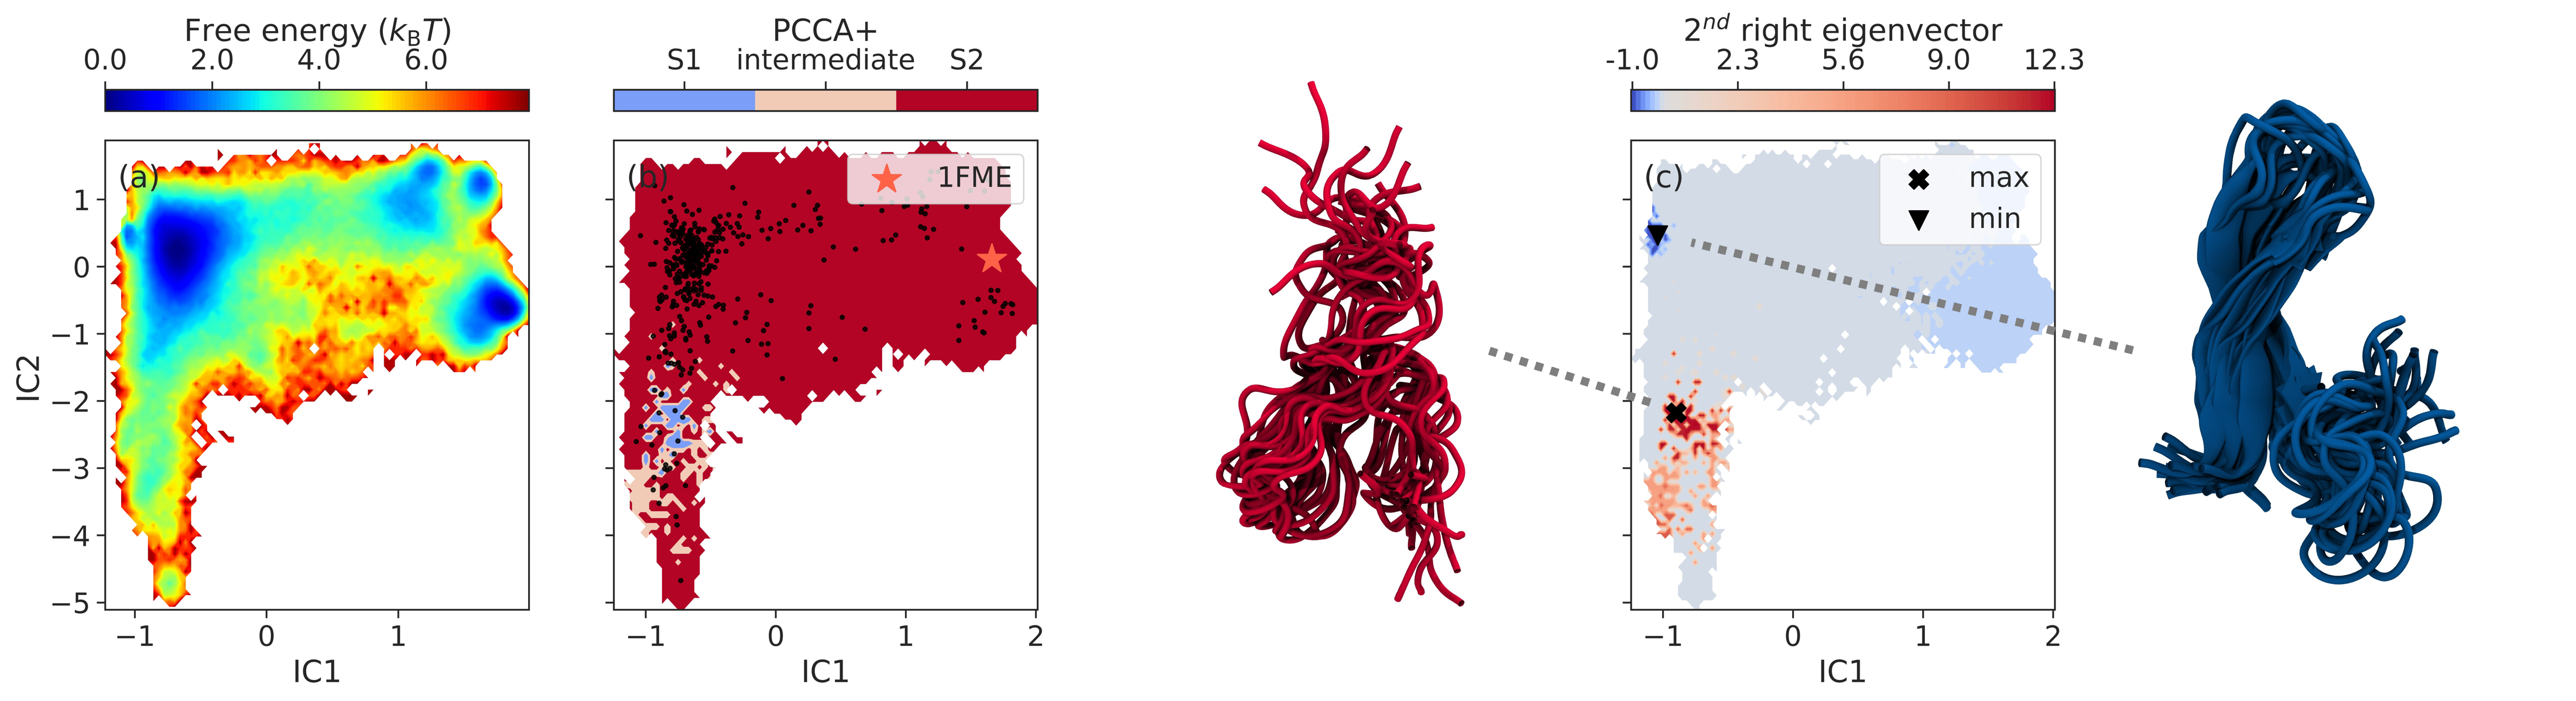
\includegraphics[width=\columnwidth]{SI_figures/BBA_227_SI-2.png}
    \caption{\textsc{BBA,  model 5 free energy surface}. See the caption for figure \ref{si_fig:BBA_24_2}.}
    \label{si_fig:BBA_227_2}
\end{figure}

\begin{figure}[h]
    \centering
    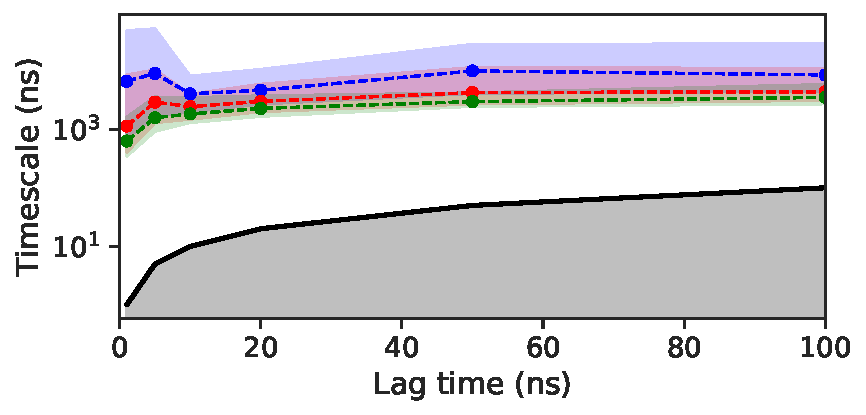
\includegraphics[height=0.15\textheight]{SI_figures/BBA_227_its.pdf}
    \caption{\textsc{BBA, model 5 validation}. See the caption for  figure \ref{si_fig:BBA_24_3}.}
    \label{si_fig:BBA_227_3}
\end{figure}

\FloatBarrier
\clearpage


\subsection{BBA model 6}

This model has the largest median $t_{2}$ after Bayesian optimisation of $\mathrm{VAMP2}_{eq}(2)$.

\begin{figure}[h]
    \centering
    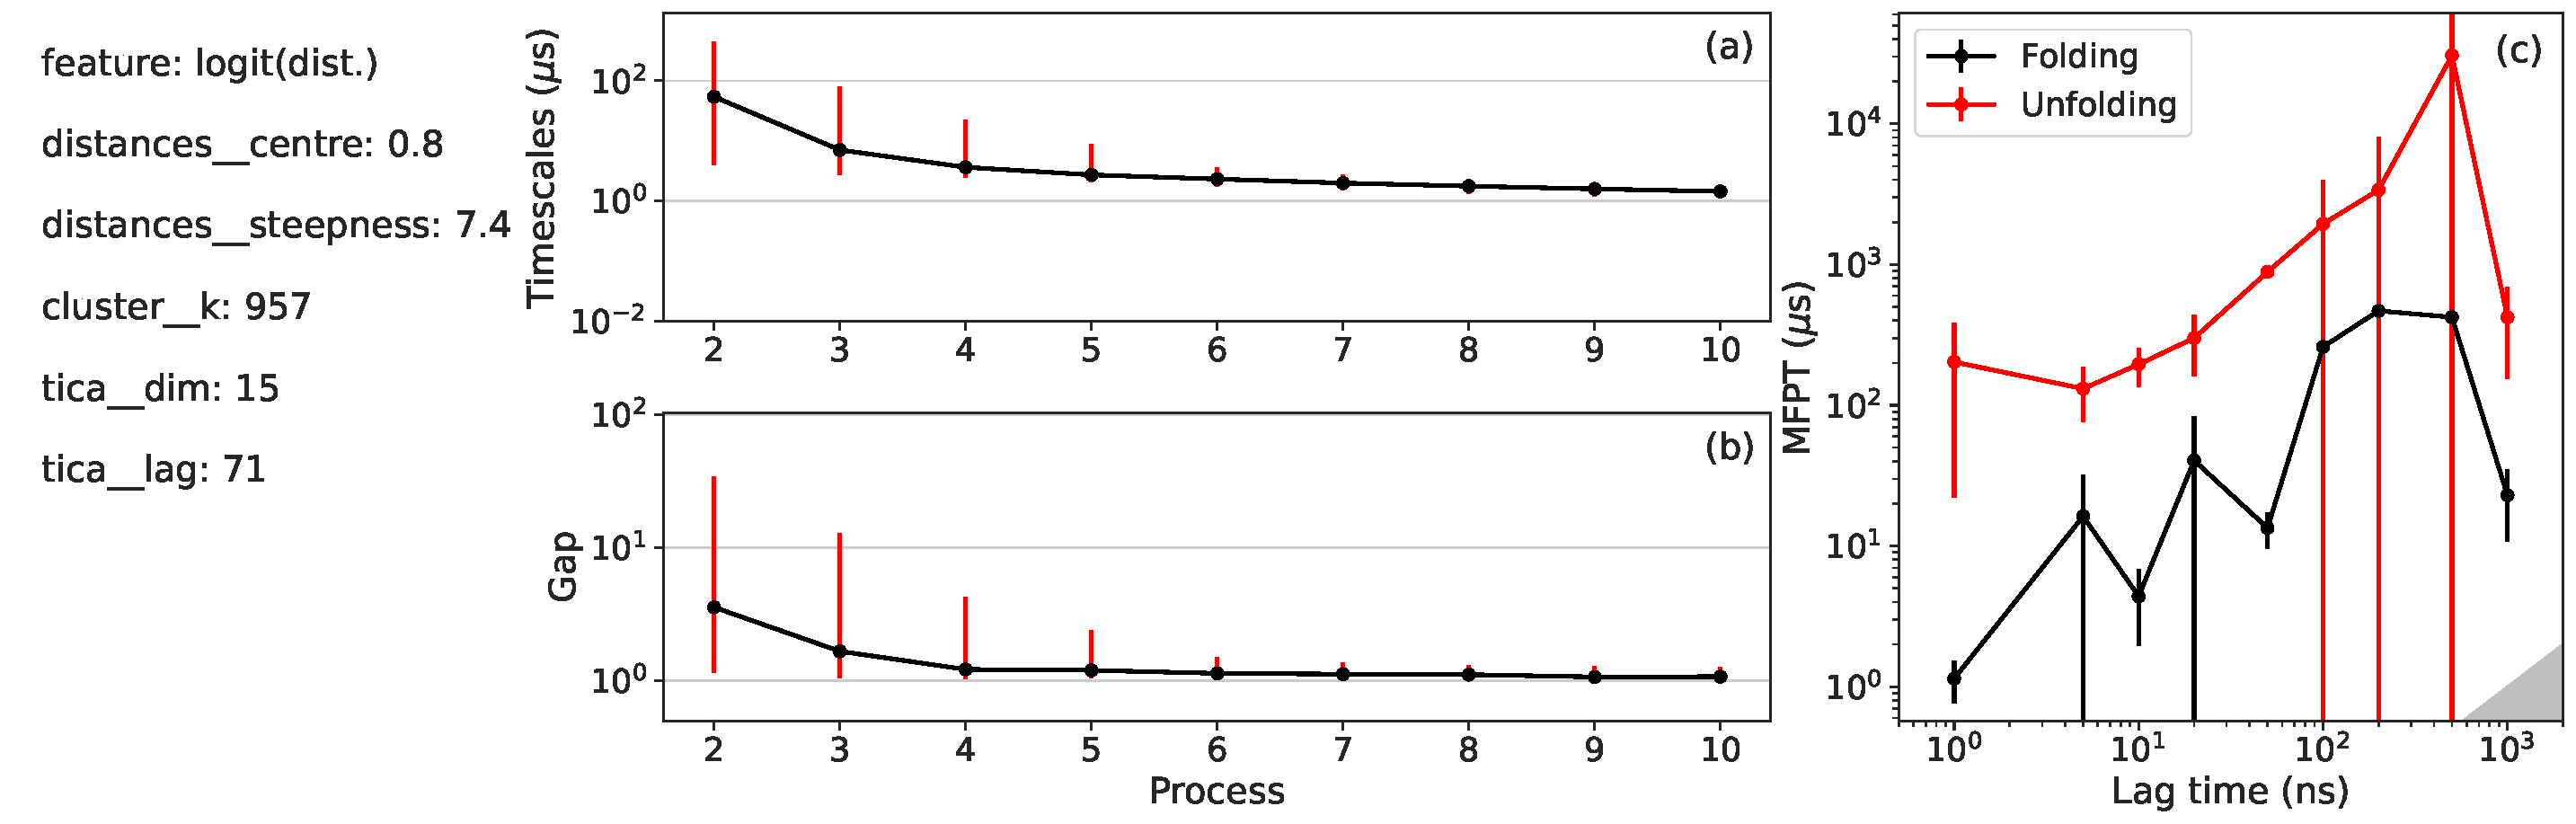
\includegraphics[width=\columnwidth]{SI_figures/BBA_185_SI-1.pdf}
    \caption{\textsc{BBA,  model 6 timescales}. See the caption for figure \ref{si_fig:BBA_24_1}.}
    \label{si_fig:BBA_185_1}
\end{figure}

\begin{figure}[h]
    \centering
    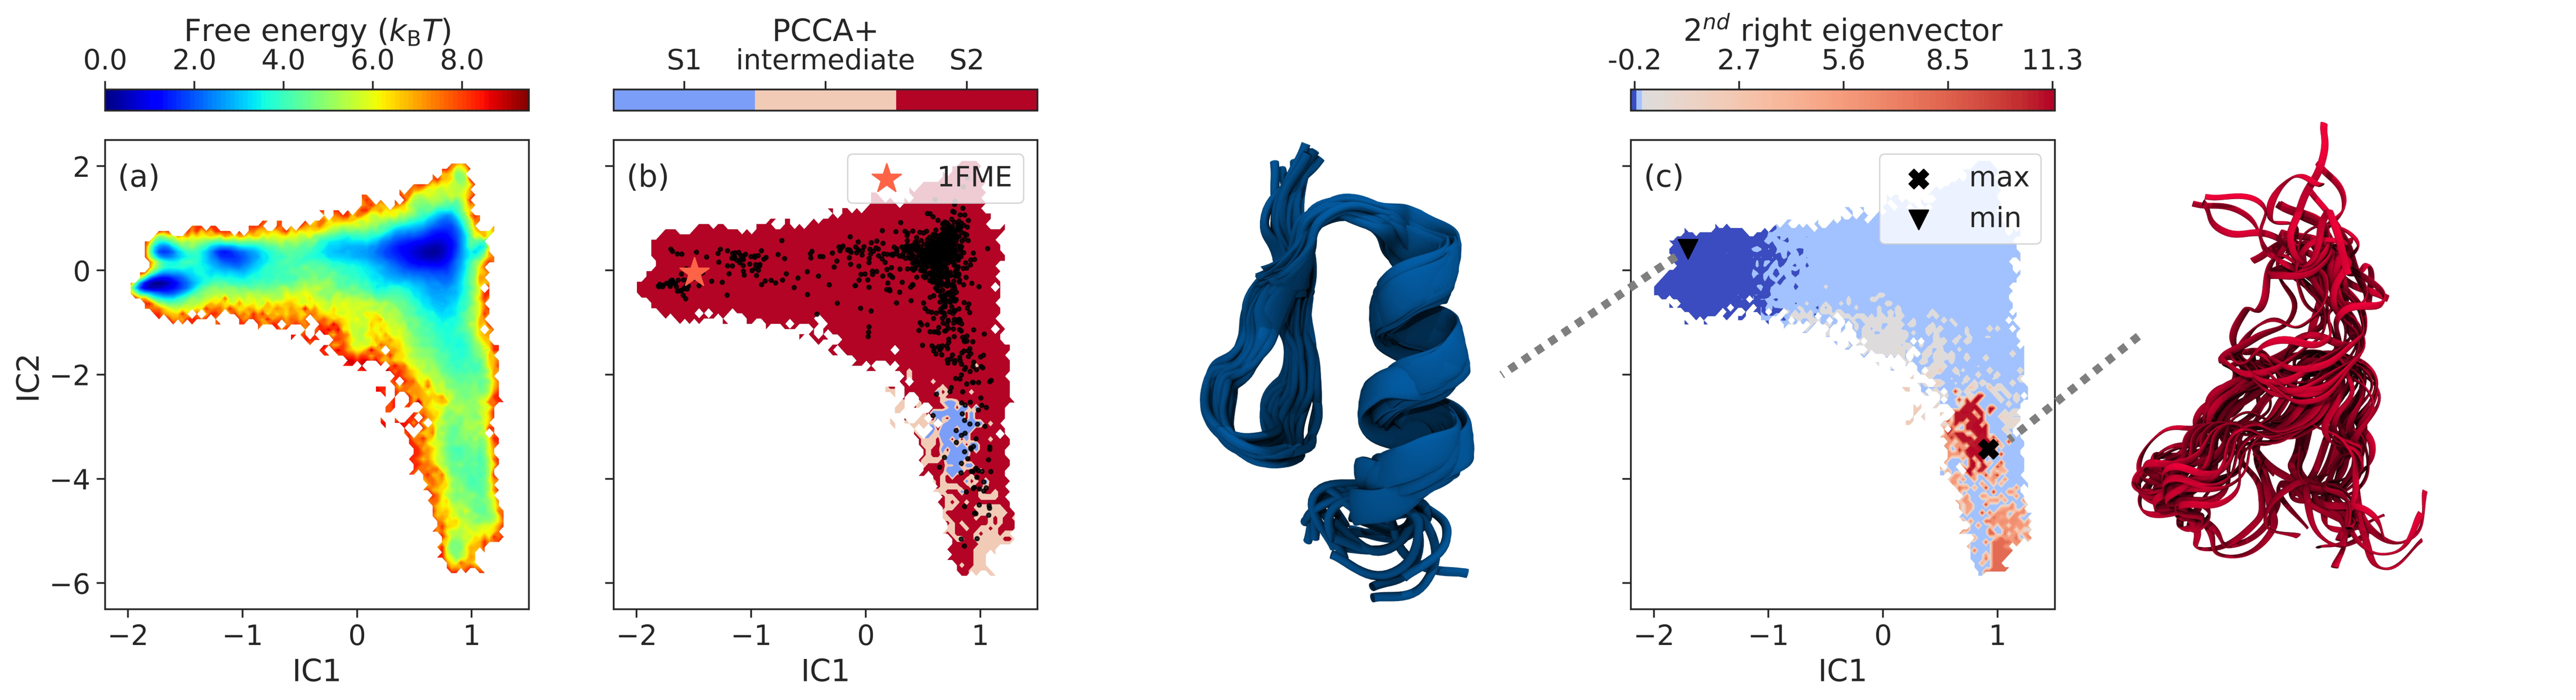
\includegraphics[width=\columnwidth]{SI_figures/BBA_185_SI-2.png}
    \caption{\textsc{BBA,  model 6 free energy surface}. See the caption for figure \ref{si_fig:BBA_24_2}.}
    \label{si_fig:BBA_185_2}
\end{figure}

\begin{figure}[h]
    \centering
    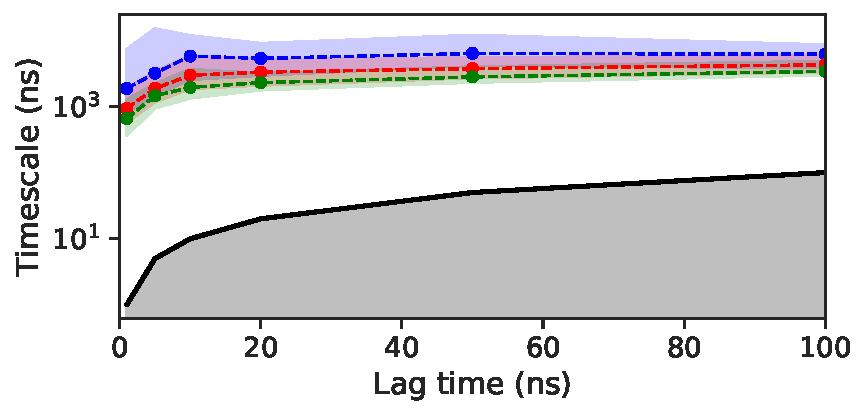
\includegraphics[height=0.15\textheight]{SI_figures/BBA_185_its.pdf}
    \caption{\textsc{BBA, model 6 validation}. See the caption for  figure \ref{si_fig:BBA_24_3}.}
    \label{si_fig:BBA_185_3}
\end{figure}

\FloatBarrier
\clearpage


\subsection{Multi-objective optimisation}

\begin{figure}[ht]
    \centering
    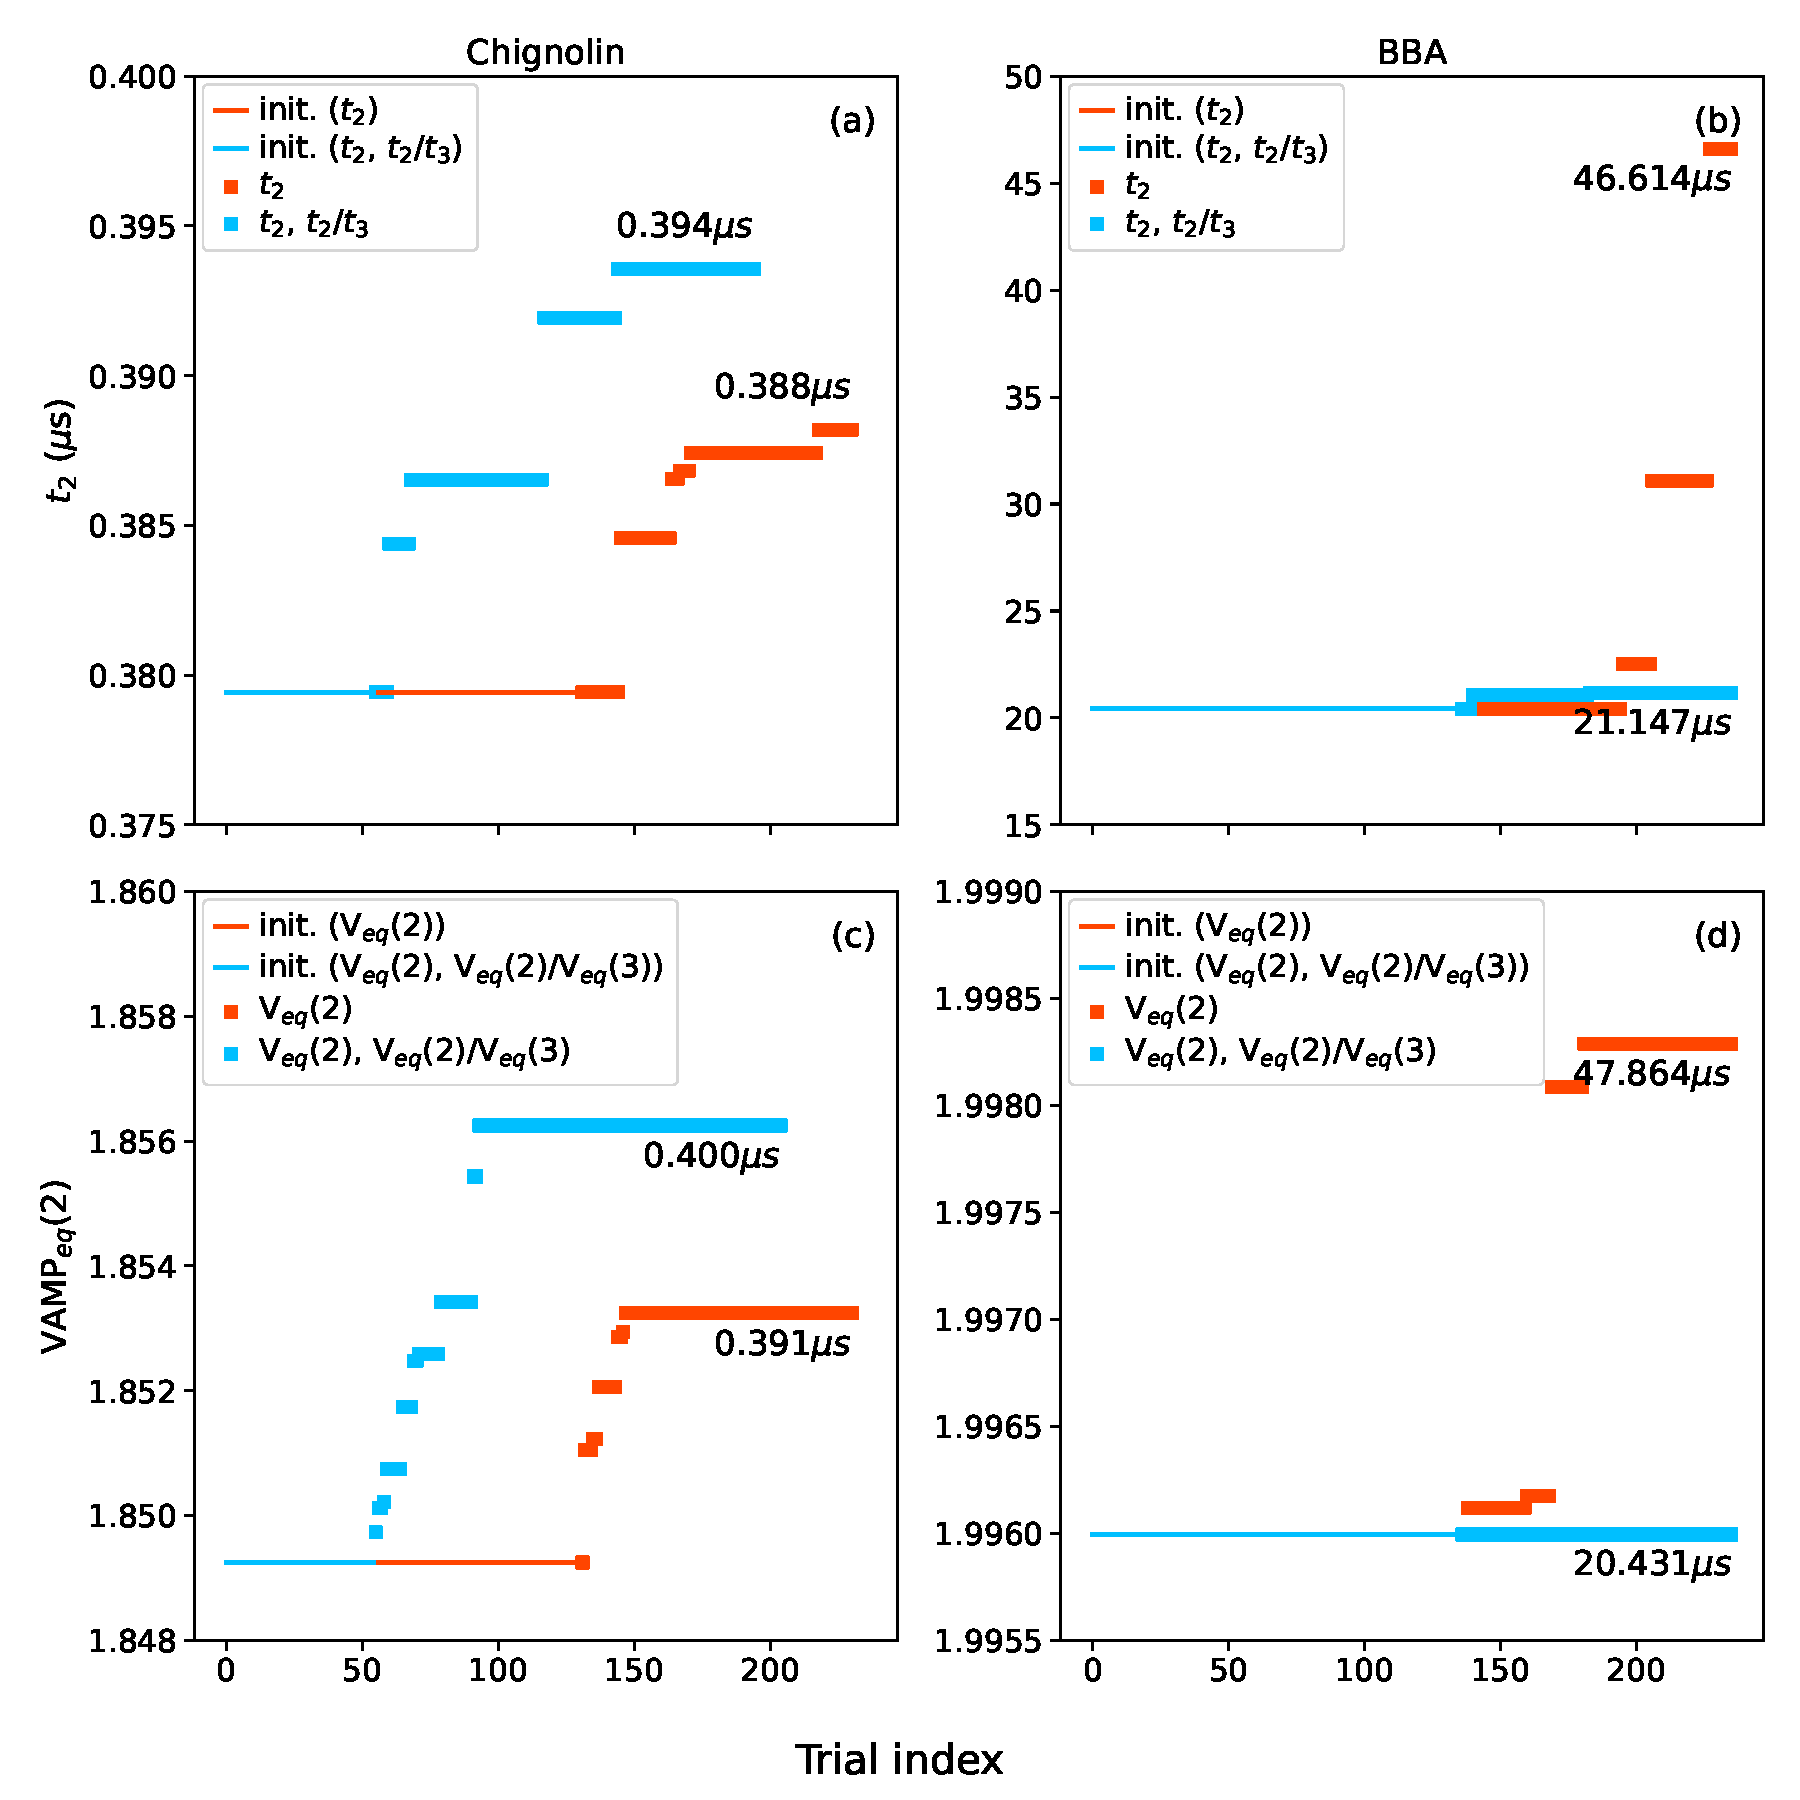
\includegraphics[width=\columnwidth]{results3/optimisation_summary.pdf}
    \caption{\textsc{Optimization of MSMs of Chignolin and BBA}. The vertical axis is the optimization objective, the horizontal axis is the trial number. The thin line refers to the incumbent over the initialization data (`init.'), and the squares are the incumbent at each trial number. Panels (a) and (c) refer to Chignolin, (b) and (d) to BBA. Panels (a) and (b) refer to Bayesian optimization with either $t_{2}$  (red), or dual-objective optimization of both $t_{2}$ and the timescale gap, $t_{2}/t_{3}$.  Panels (c) and (d) refer to optimization of  $\mathrm{VAMP2}_{eq}(2)$ (red) and dual-objective optimization of both  $\mathrm{VAMP2}_{eq}(2)$ and $\mathrm{VAMP2}_{eq}(2)/\mathrm{VAMP2}_{eq}(3)$. The optimized values of $t_2$ are shown as labels. }
    \label{fig:optimisation_trials}
\end{figure}


\begin{figure}[ht]
    \centering
    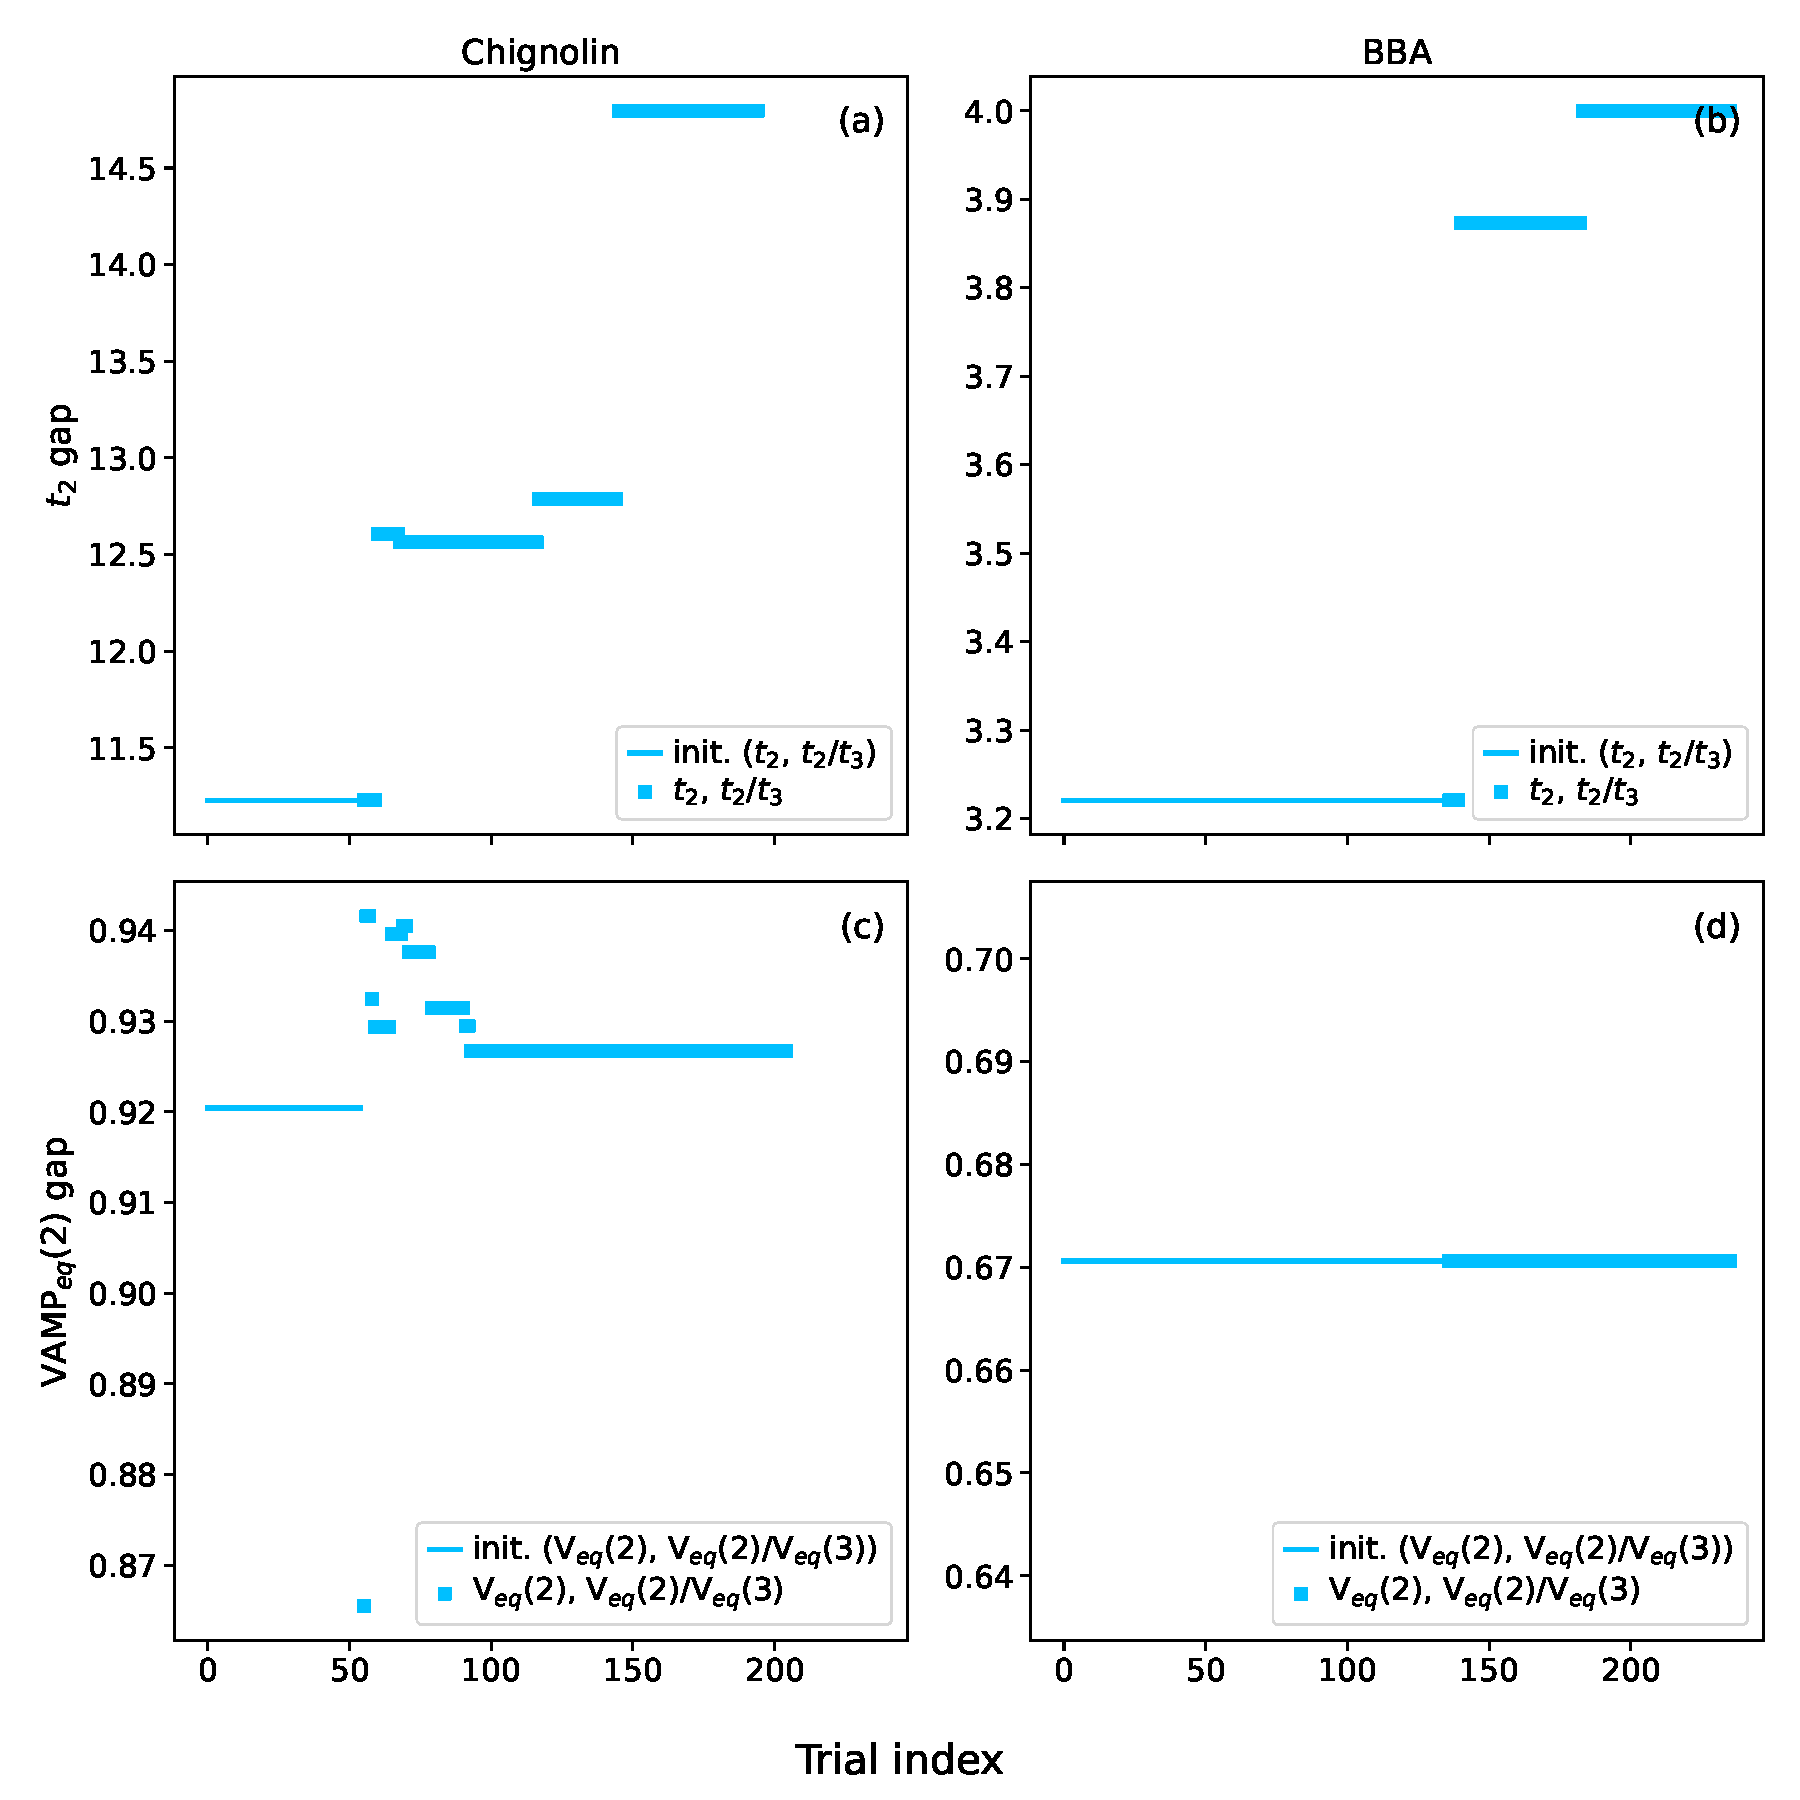
\includegraphics[width=0.8\textwidth]{SI_figures/optimisation_gap_summary.pdf}
    \caption{\textsc{Optimisation of the timescale and VAMP2$_{eq}$ gap.} The blue dots show the incumbent gap during optimisation (shown only for the multi-objective optimisation). Panels (a) and (b) refer to the timescale gap $t_2/t_3$ while panels (c) and (d) refer to the VAMP2$_{eq}(2)$/VAMP2$_eq(3)$. Panels (a) and (c) are for Chignolin optimisation while the panels (b) and (d) refer to BBA.}
    \label{fig:gap_optimiation}
\end{figure}

\FloatBarrier
\clearpage

% % \section{Summary of trial results}

% % \begin{table}[h]
% %     \centering
% %     \begin{tabular}{|l|c|}
% %        Number of  attempted trials   & 140 \\
% %        Number of trials with at least one successful bootstrap & 136 \\
% %        Smallest number of successful bootstrap trails & 88
% %     \end{tabular}
% %     \caption{\textsc{Trial statistics}. Results refers to a $\tau=\SI{41}{\nano\second}$ and the folding timescale ($t_{2}$).}
% %     \label{tab:summary_stats_1}
% % \end{table}


% % \begin{table}[h]
% %     \centering
% %     \begin{tabular}{l|l|l|c}
% %         Feature & Contact scheme & Distance transformation & Num. trials  \\
% %         \toprule
% %         Dihedrals & - & - & 20 \\
% %         Contact distances & $\alpha-$Carbon & Linear & 20 \\
% %         Contact distances & Closest-heavy & Linear & 20 \\
% %         Contact distances & $\alpha-$Carbon & Logistic & 36 \\
% %         Contact distances & Closest-heavy & Logistic & 40 \\
% %     \end{tabular}
% %     \caption{\textsc{Trial statistics per feature for BBA}. Results refers to a $\tau=\SI{41}{\nano\second}$ and the folding timescale ($t_{2}$). `Num. trials' refers to the number of trials with at least one successful bootstrap.}
% %     \label{tab:summary_stats_2}
% % \end{table}



% % \begin{table}[h]
% %     \centering
% %     \begin{tabular}{l|l|l|c}
% %         Feature & Contact scheme & Distance transformation & Num. trials  \\
% %         \toprule
% %         Dihedrals & - & - & 20? \\
% %         Contact distances & $\alpha-$Carbon & Linear & 20? \\
% %         Contact distances & Closest-heavy & Linear & 20? \\
% %         Contact distances & $\alpha-$Carbon & Logistic & 40? \\
% %         Contact distances & Closest-heavy & Logistic & 40? \\
% %     \end{tabular}
% %     \caption{\textsc{Trial statistics per feature for Chignolin}. Results refers to a $\tau=$ [Ryan] and the folding timescale ($t_{2}$). `Num. trials' refers to the number of trials with at least one successful bootstrap.}
% %     \label{tab:summary_stats_2}
% % \end{table}

% % \begin{figure}
% %     \centering
% %     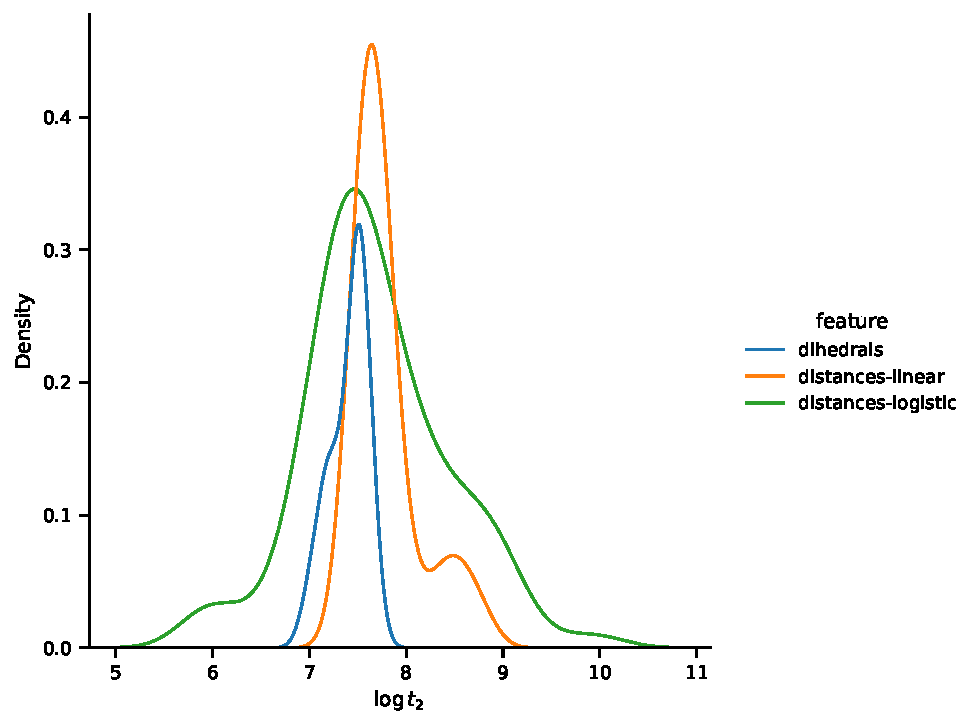
\includegraphics{figures/timescale_dist_summary.pdf}
% %     \caption{\textsc{Distribution of the folding timescale}. The log of $t_2$, for each feature. }
% %     \label{fig:ts_distribution}
% % \end{figure}

% \section{Choosing the Markov lag time}

% The Markov lag time was estimated from the \num{136} successful trials.  

% \begin{figure}[h]
%     \centering
%     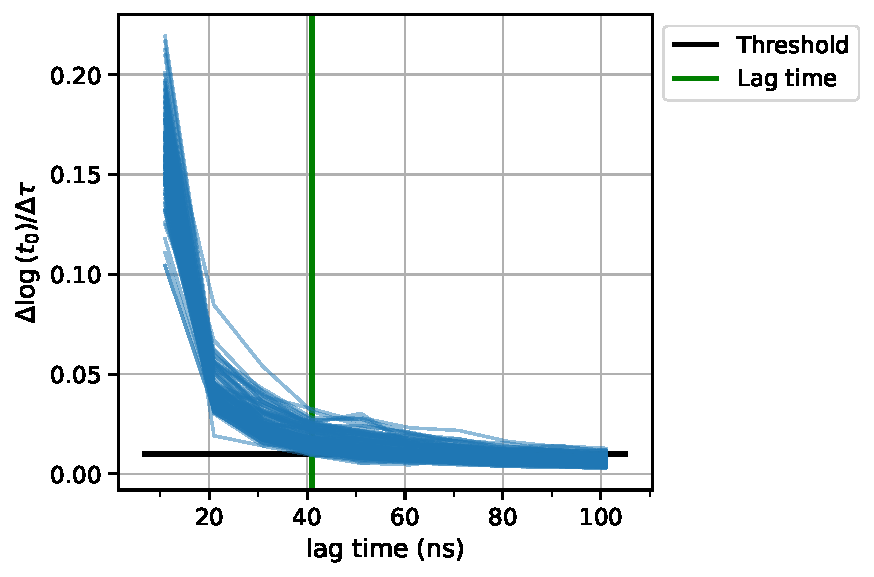
\includegraphics[width=0.8\textwidth]{figures/BBA_timescale_gradient.pdf}
%     \caption{\textsc{Gradient of $t_{2}$ with respect to the Markov lag time.} Each is calculated according to equation~\ref{eqn:choose_lag_1}.  The black horizontal line is the gradient threshold ($\log{1.01}$) and the vertical green line is the selected lag time, selected according to equation~\ref{eqn:choose_lag_2}. }
%     \label{fig:choose_lag}
% \end{figure}

% \section{How does the number of scored processes affect model selection?}

% \begin{figure}
%     \centering
%     \includegraphics[width=1.0\textwidth]{figures/vampeq_rank_vs_proc_pairplot.pdf}
%     \caption{\textsc{Pair plot of $\operatorname{VAMP2}_{eq}(k)$ rank with different numbers of scored processes}. The panel at position $(0,1)$ plots the rank according to$\operatorname{VAMP2}_{eq}(2)$ against the  rank according to$\operatorname{VAMP2}_{eq}(3)$, and similarly for other positions. This }
%     \label{fig:vampeq_rank_vs_proc_pairplot}
% \end{figure}

\subsection{VAMP2$_{eq}$ vs Lag time.}

\begin{figure}
    \centering
    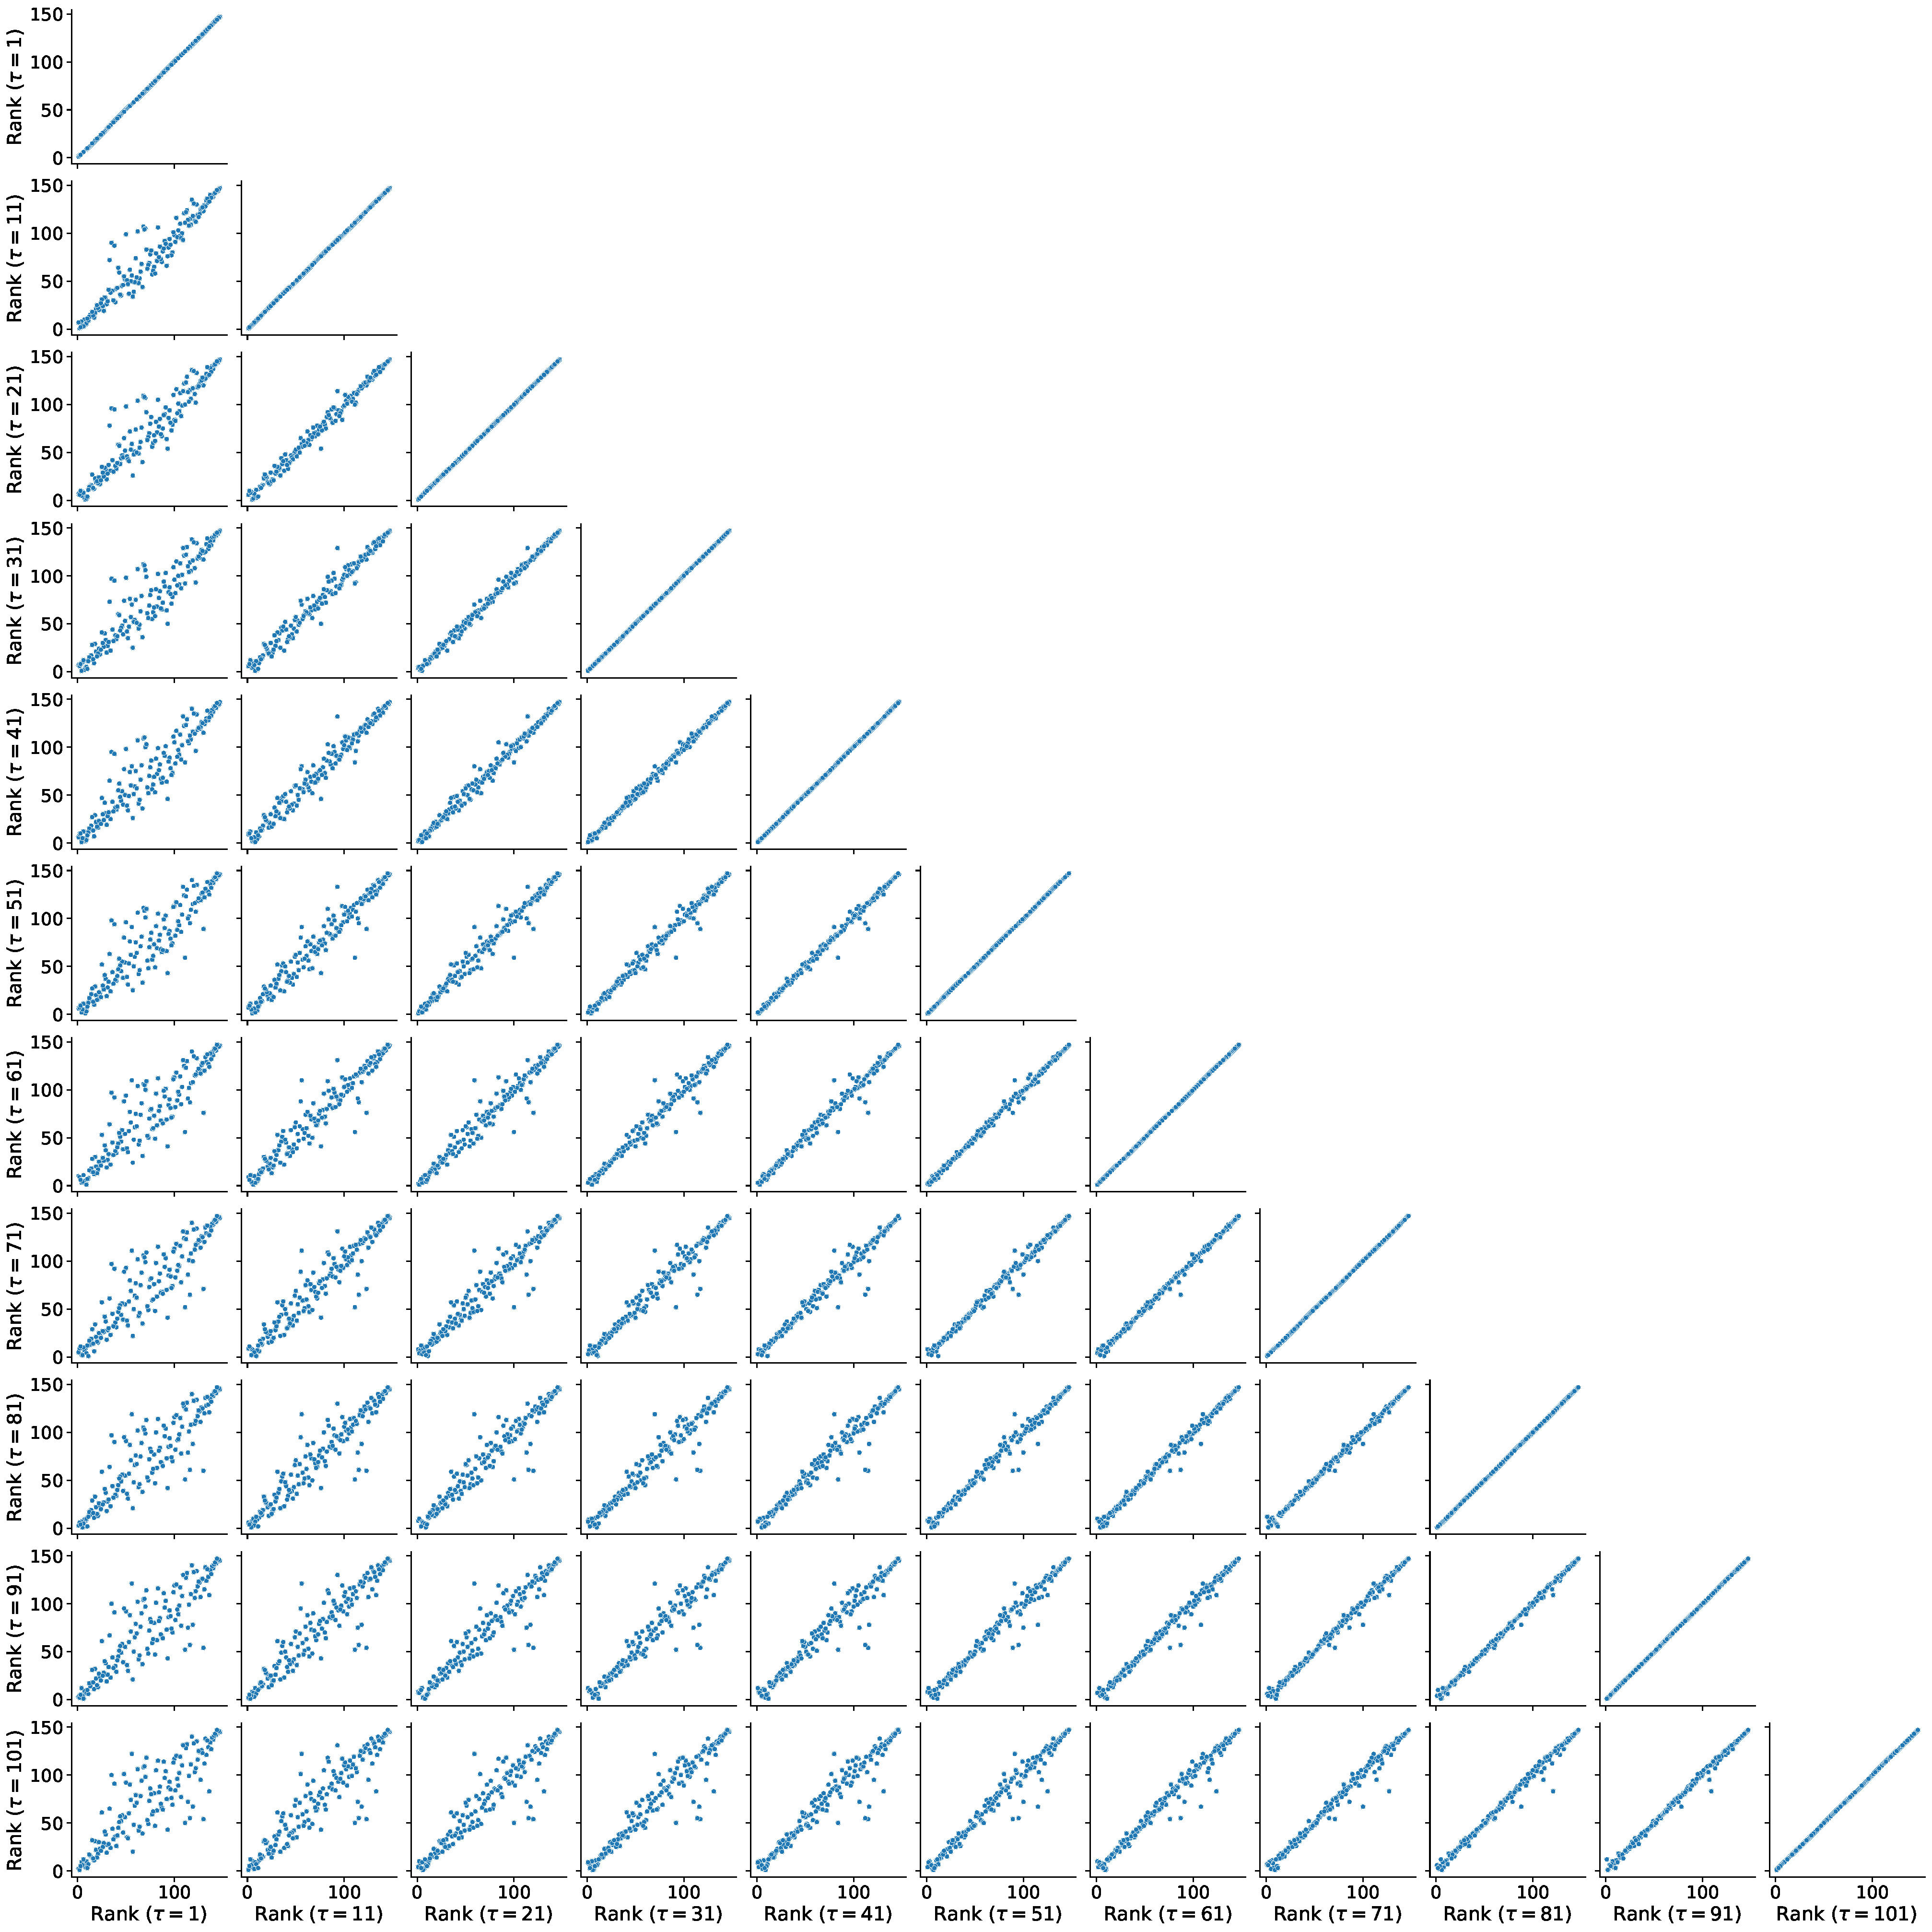
\includegraphics[width=1.0\textwidth]{SI_figures/1fme_vampeq_rank_vs_lag_pairplot_k2.pdf}
    \caption{\textsc{Pair plot of $\operatorname{VAMP2}_{eq}(k=2)$ rank with different lag times.} The panel at position $(0,1)$ plots the rank according to$\operatorname{VAMP2}_{eq}(2)$ against the  rank according to$\operatorname{VAMP2}_{eq}(3)$, and similarly for other positions. This }
    \label{fig:vampeq2_rank_vs_lag_pairplot}
\end{figure}


\begin{figure}
    \centering
    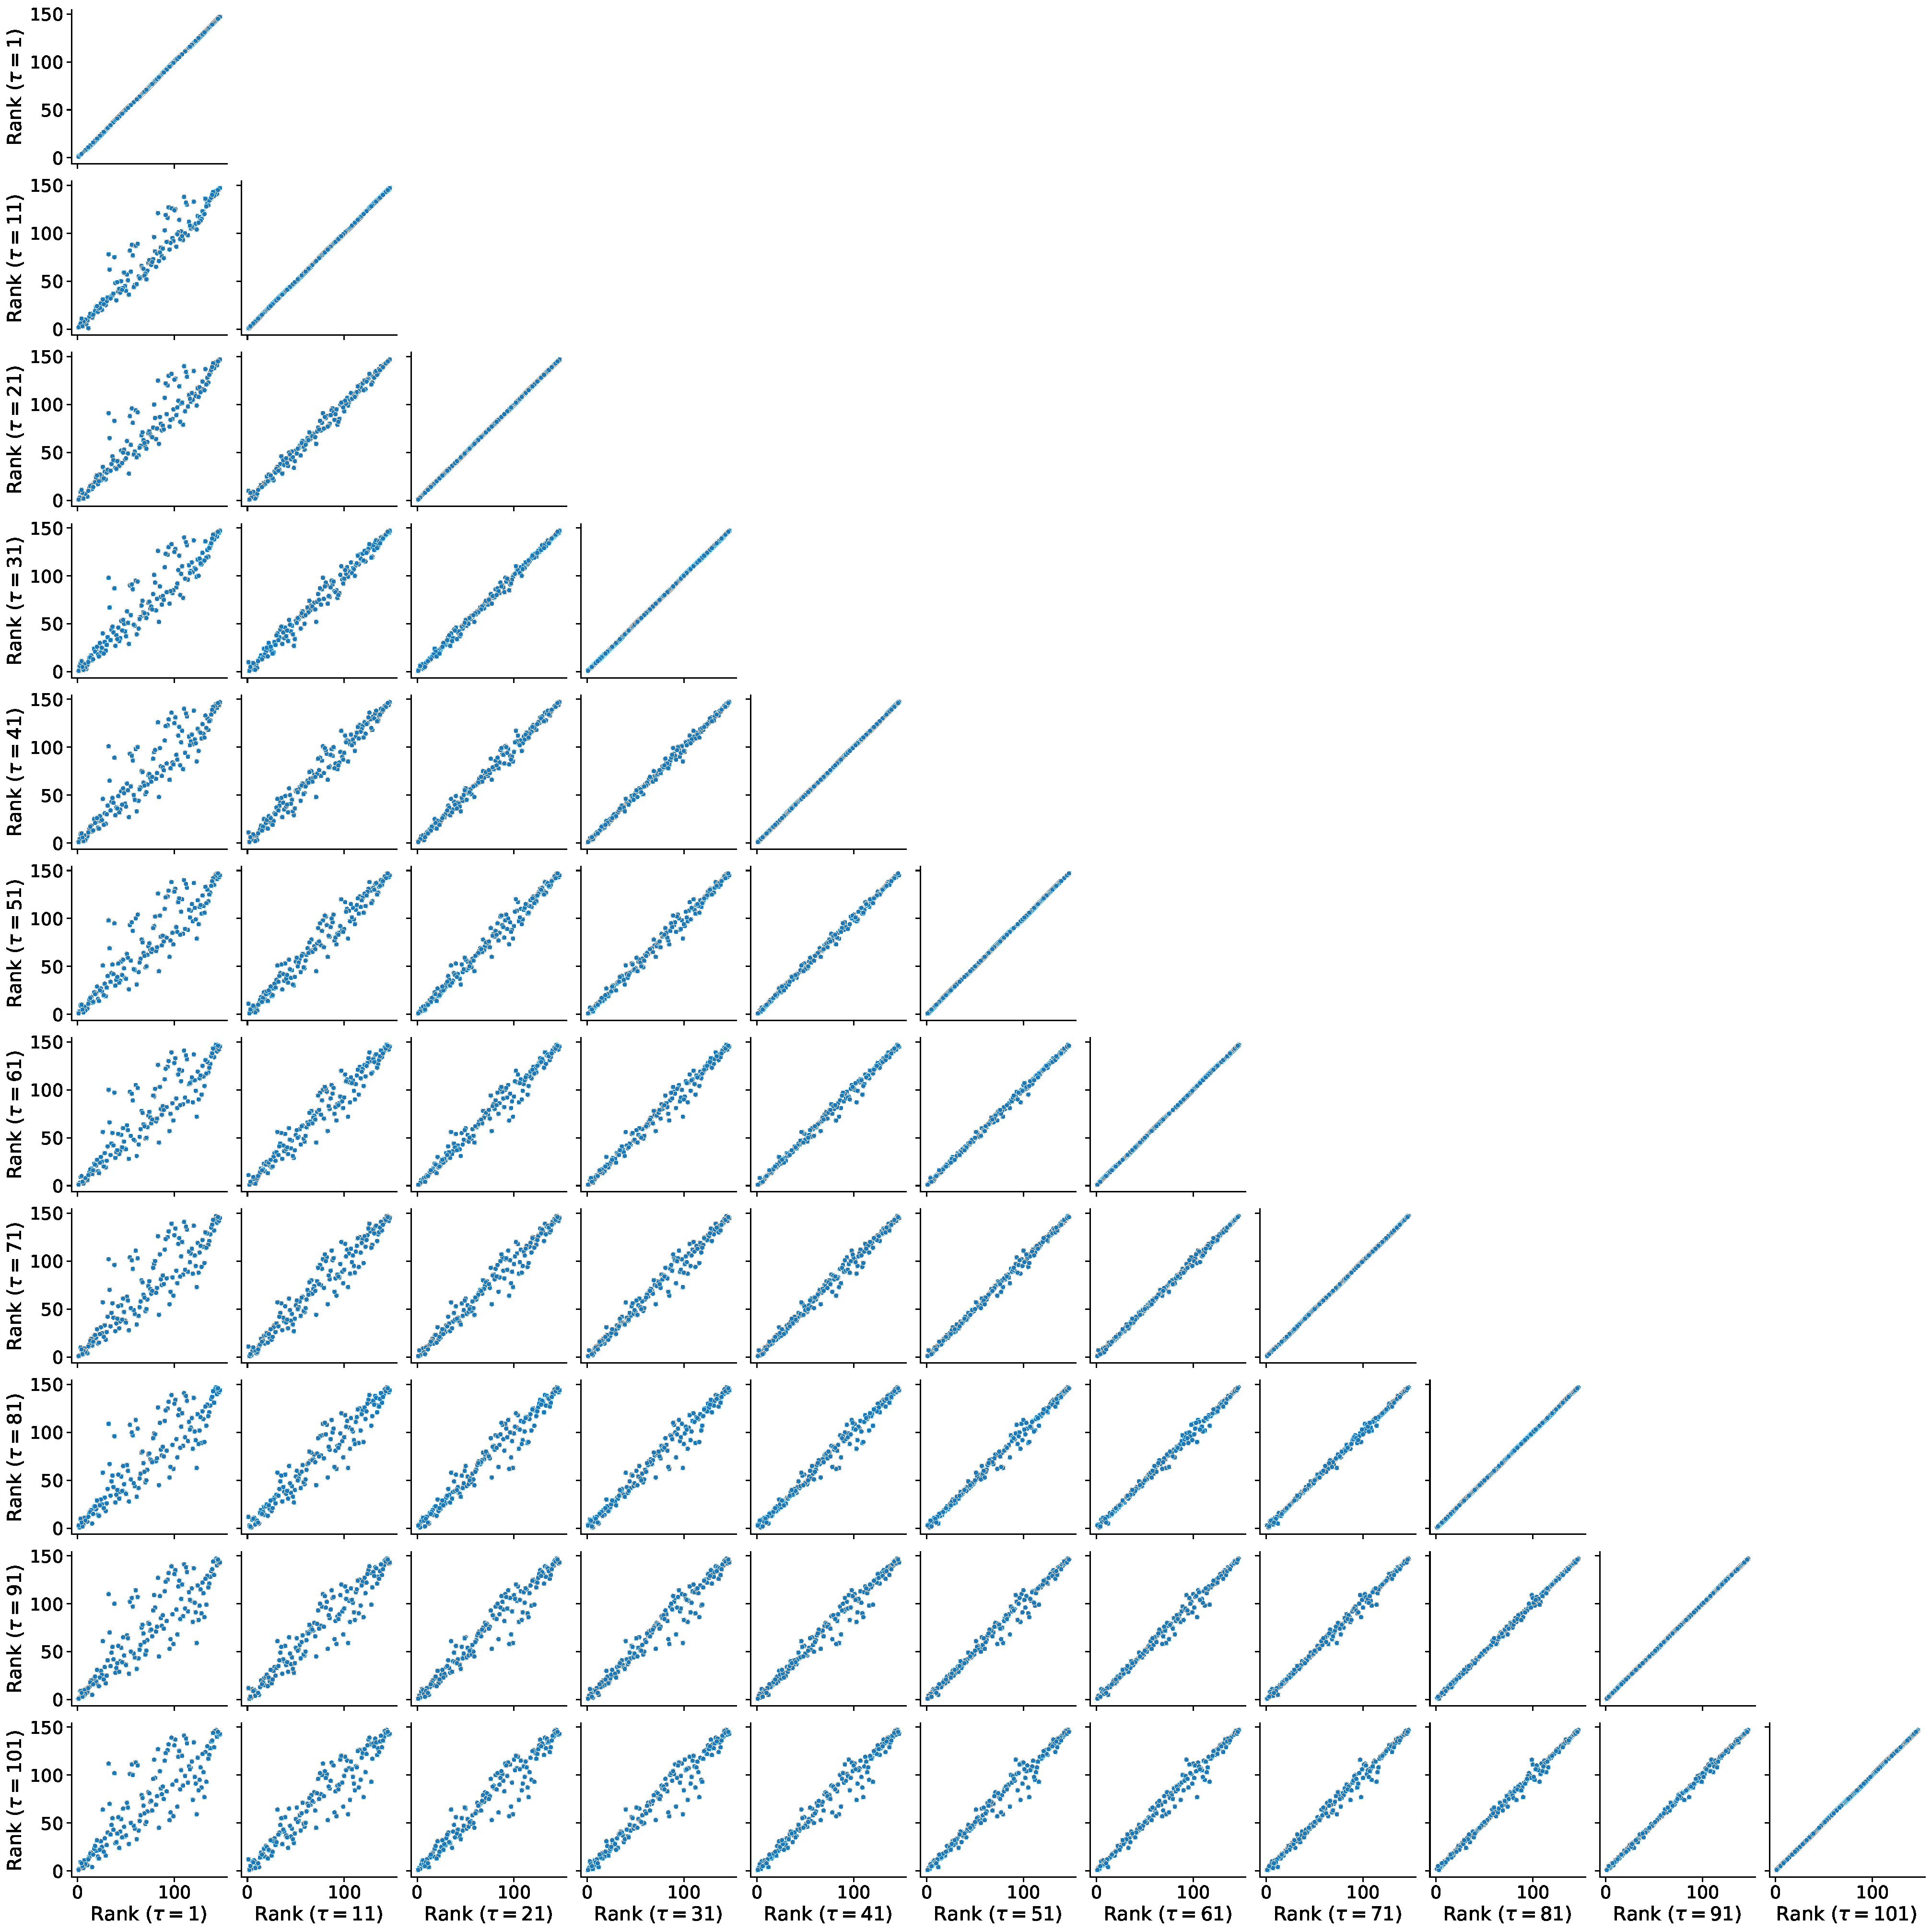
\includegraphics[width=1.0\textwidth]{SI_figures/1fme_vampeq_rank_vs_lag_pairplot_k3.pdf}
    \caption{\textsc{Pair plot of $\operatorname{VAMP2}_{eq}(k=3)$ rank with different lag times.} The panel at position $(0,1)$ plots the rank according to$\operatorname{VAMP2}_{eq}(2)$ against the  rank according to$\operatorname{VAMP2}_{eq}(3)$, and similarly for other positions. This }
    \label{fig:vampeq3_rank_vs_lag_pairplot}
\end{figure}

\begin{figure}
    \centering
    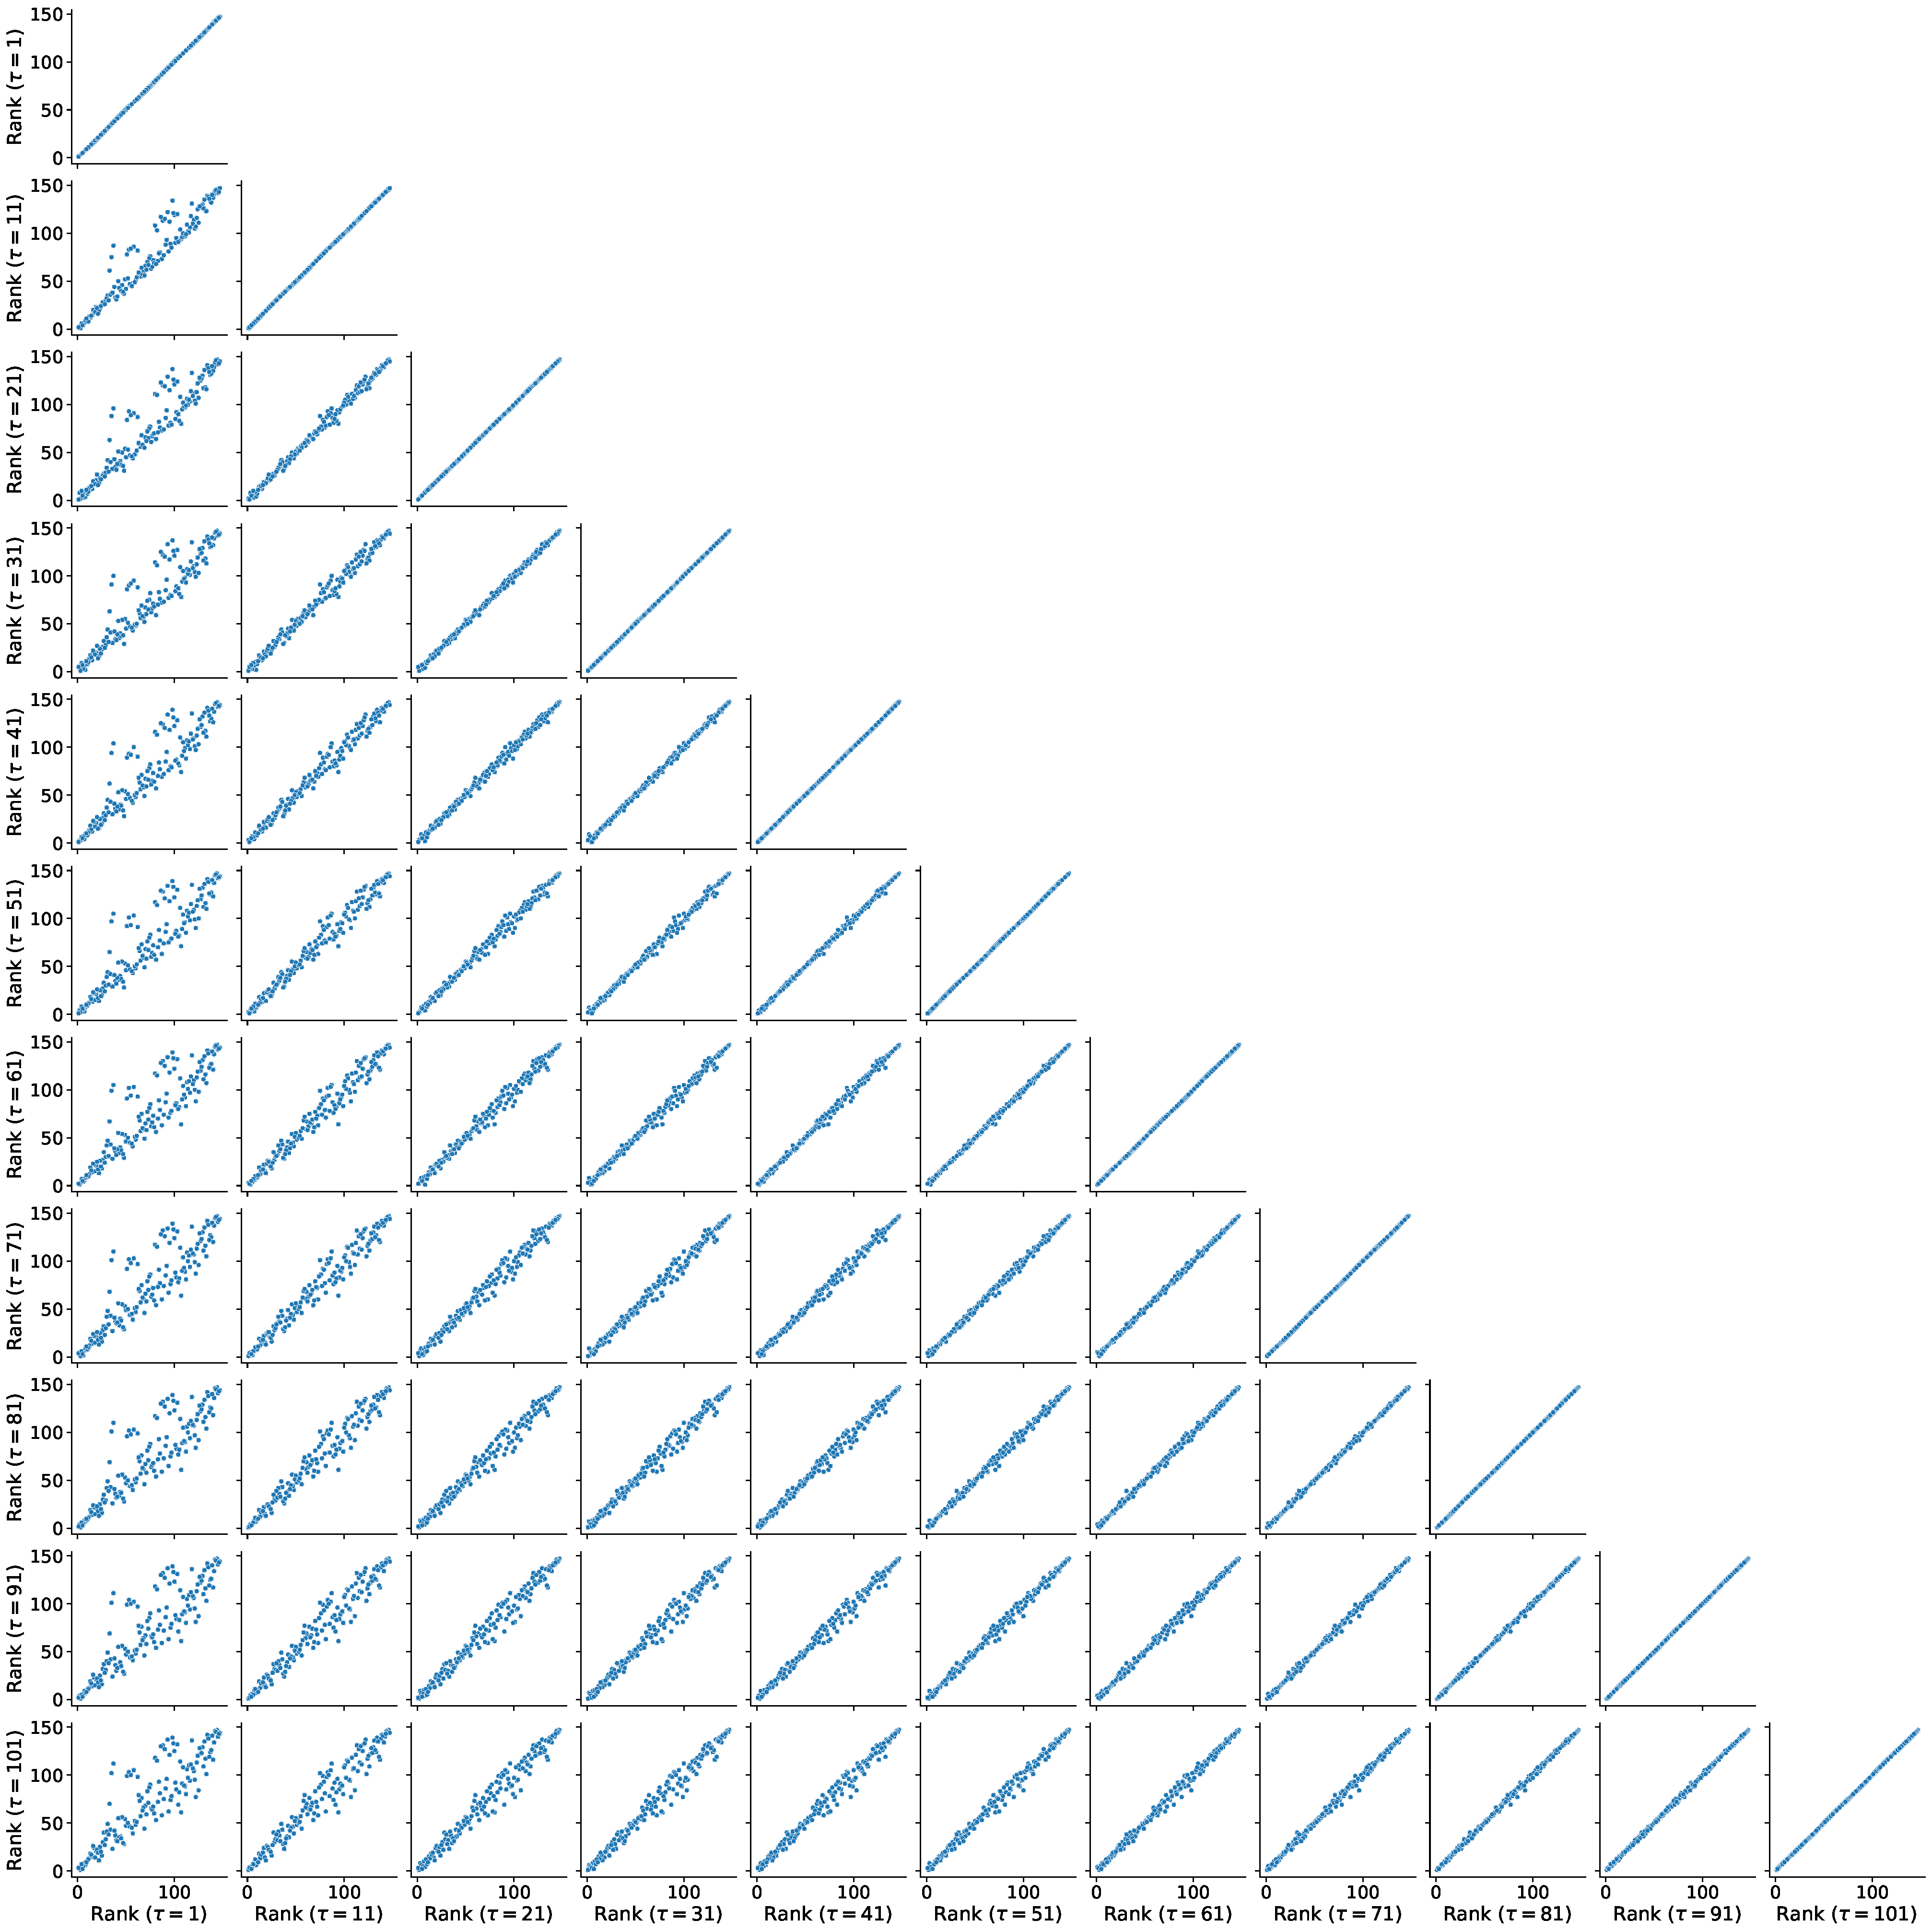
\includegraphics[width=1.0\textwidth]{SI_figures/1fme_vampeq_rank_vs_lag_pairplot_k5.pdf}
    \caption{\textsc{Pair plot of $\operatorname{VAMP2}_{eq}(k=5)$ rank with different lag times.} The panel at position $(0,1)$ plots the rank according to$\operatorname{VAMP2}_{eq}(2)$ against the  rank according to$\operatorname{VAMP2}_{eq}(3)$, and similarly for other positions. This }
    \label{fig:vampeq5_rank_vs_lag_pairplot}
\end{figure}

\begin{figure}
    \centering
    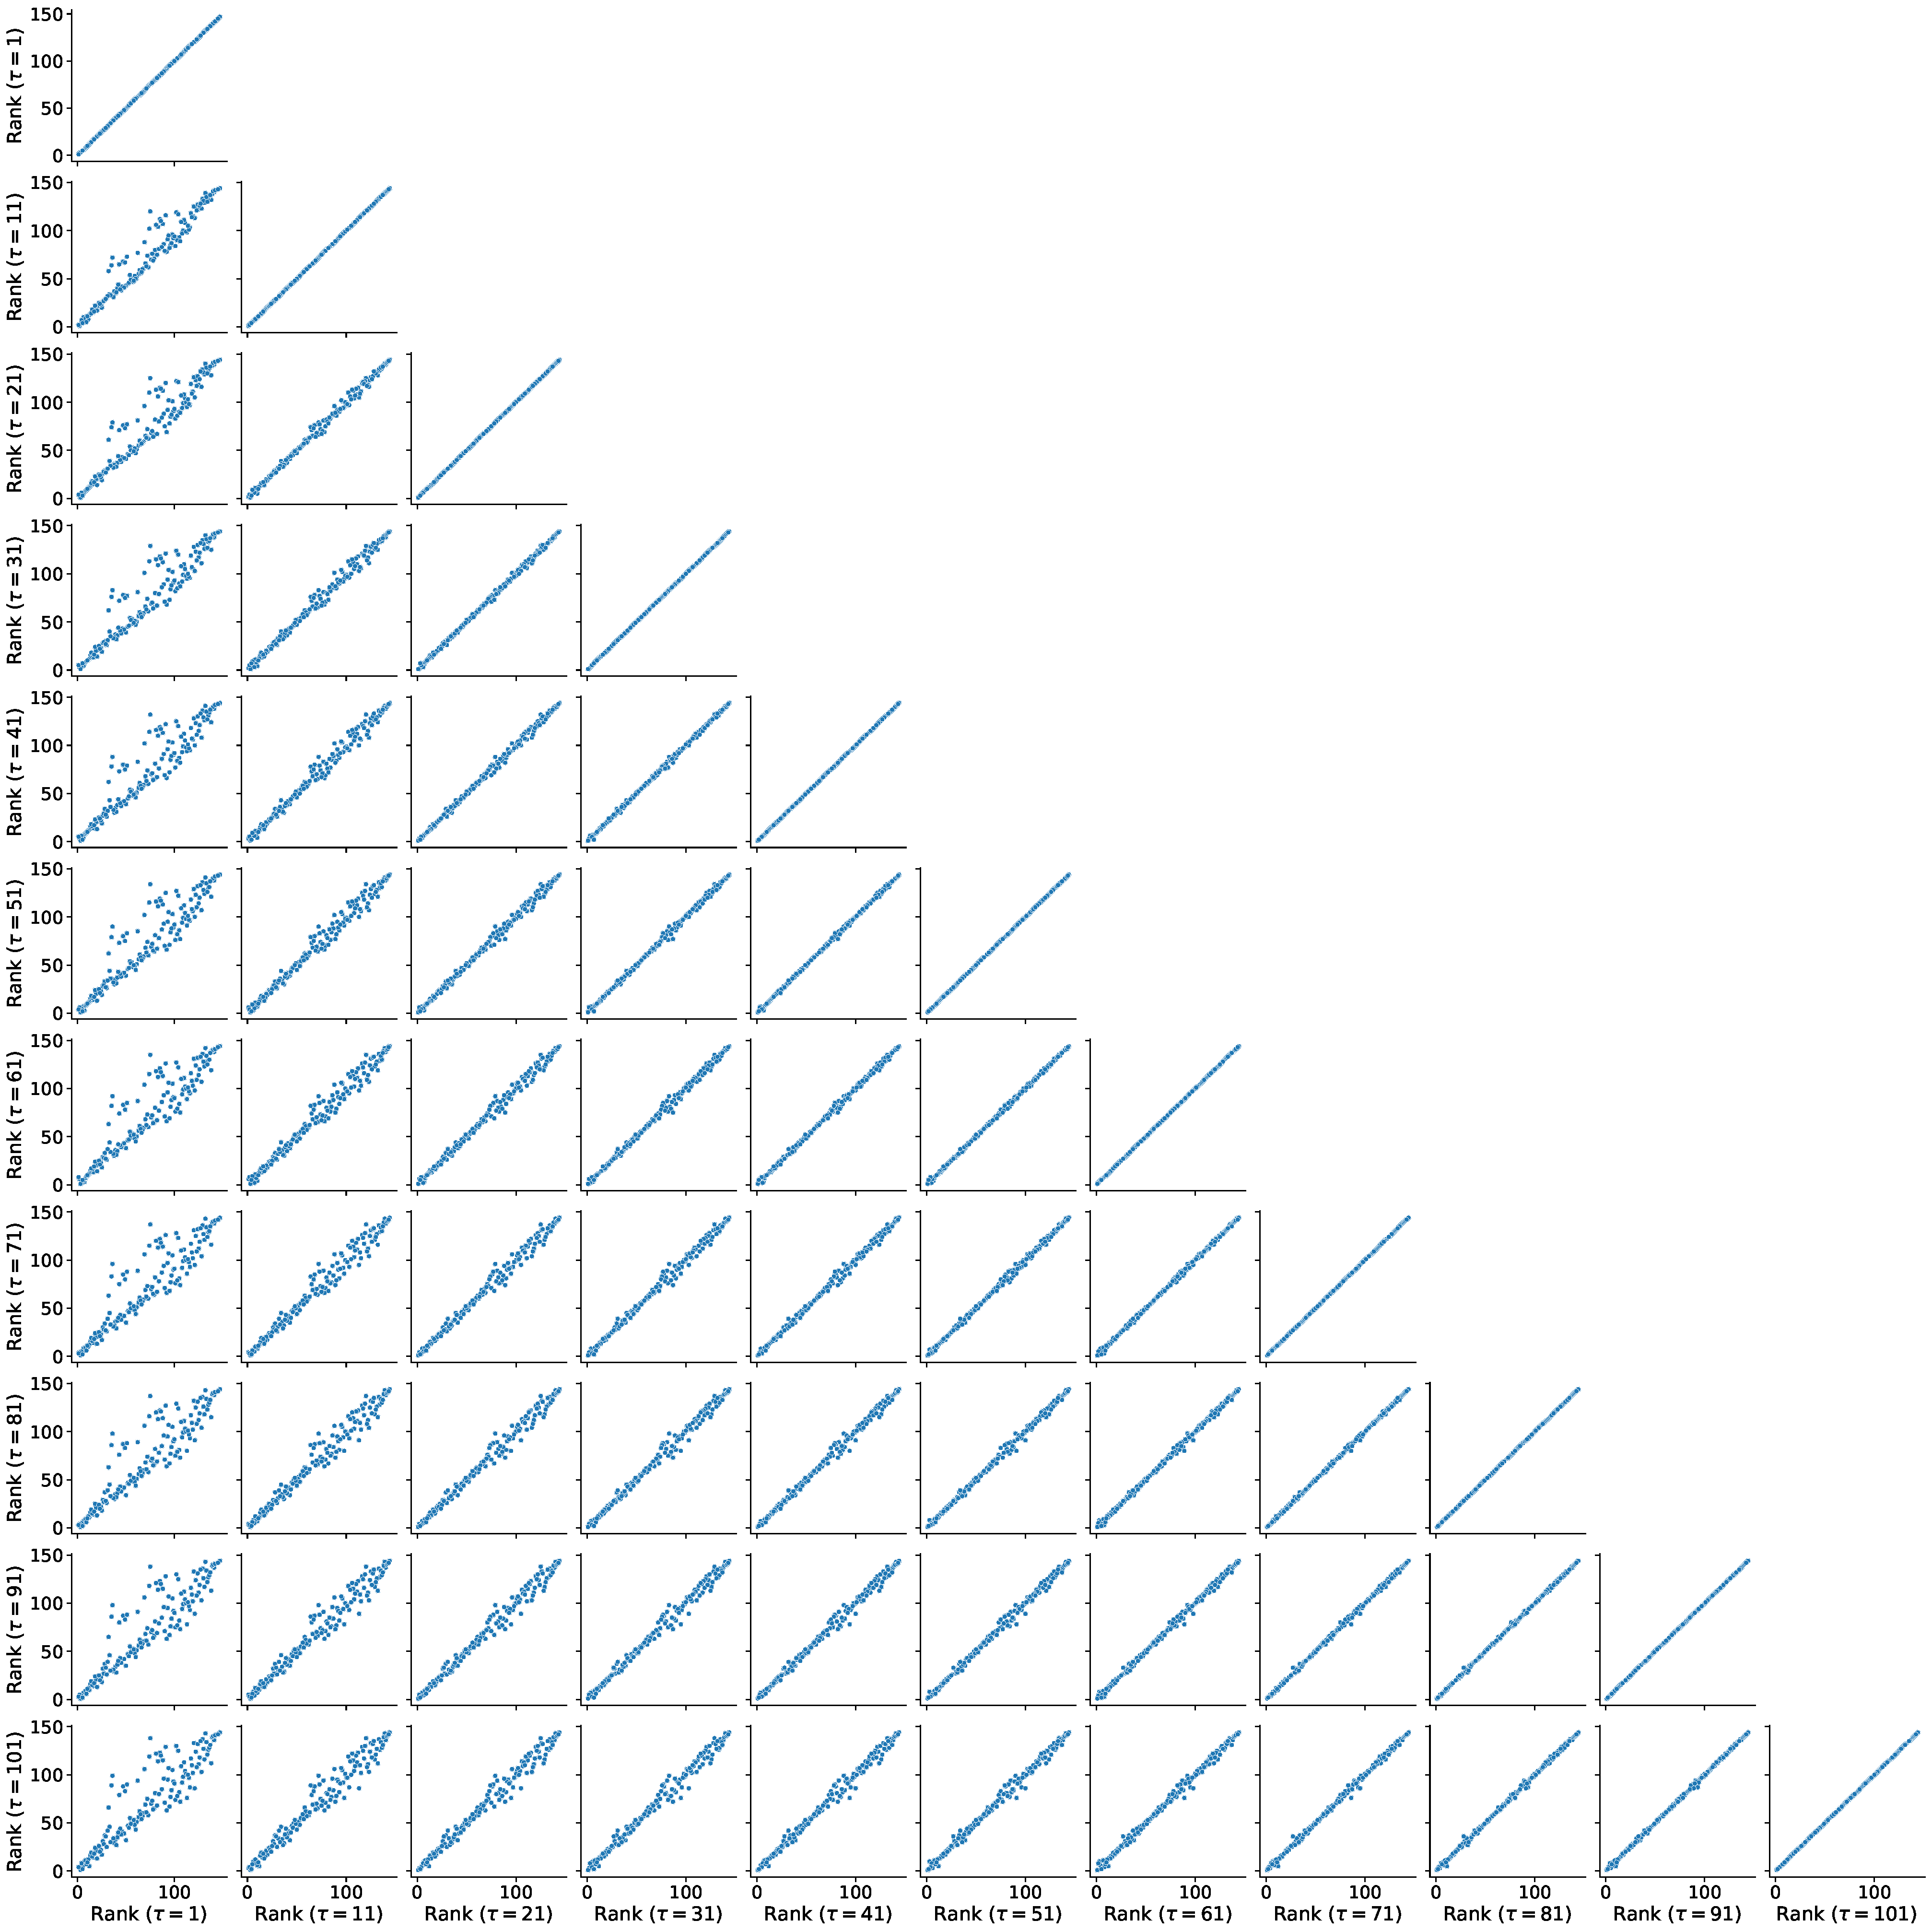
\includegraphics[width=1.0\textwidth]{SI_figures/1fme_vampeq_rank_vs_lag_pairplot_k10.pdf}
    \caption{\textsc{Pair plot of $\operatorname{VAMP2}_{eq}(k=5)$ rank with different lag times.} The panel at position $(0,1)$ plots the rank according to$\operatorname{VAMP2}_{eq}(2)$ against the  rank according to$\operatorname{VAMP2}_{eq}(3)$, and similarly for other positions. This }
    \label{fig:vampeq10_rank_vs_lag_pairplot}
\end{figure}

% \section{Modelling the hyperparameter response surface}\label{sec:response_surface_fitting}


% \begin{figure}[h]
%     \centering
%     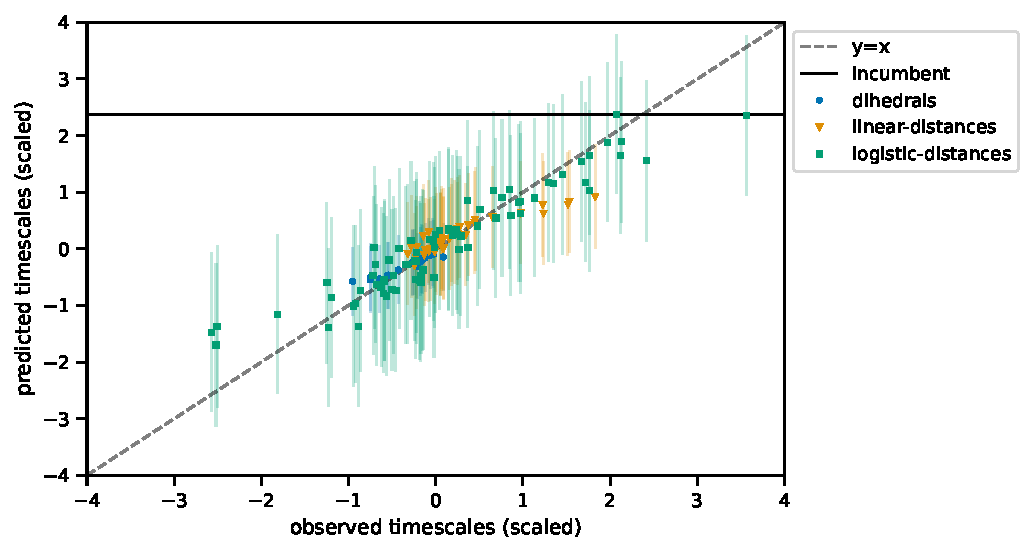
\includegraphics[width=0.8\textwidth]{figures/response_surface_predictions_ts.pdf}
%     \caption{Response surface predictions. The timescales are modelled (after a log-transform and scaling) as a Gaussian process, separately for each feature. The predictions and error bars are the $(\mu, 2\sigma)$ of the Gaussian process. The incumbent is the largest mean predicted value. }
%     \label{fig:response_surface}
% \end{figure}

% How the models were fit to the data. 

% \section{Estimating the hyperparameter relevance}\label{sec:hp_relevance_calc}

% These were chosen so as to maximize the expected improvement, i.e., the figure plots $y=f(s, c, d^{*}, m^{*}, \tau^{*}, n^{*})$ where $s^{*}, c^{*}, d^{*}, m^{*}, \tau^{*}, n^{*} = \argmax \left [f(s, c, d, m, \tau,n)\right]$.


% \begin{figure}
%     \centering
%     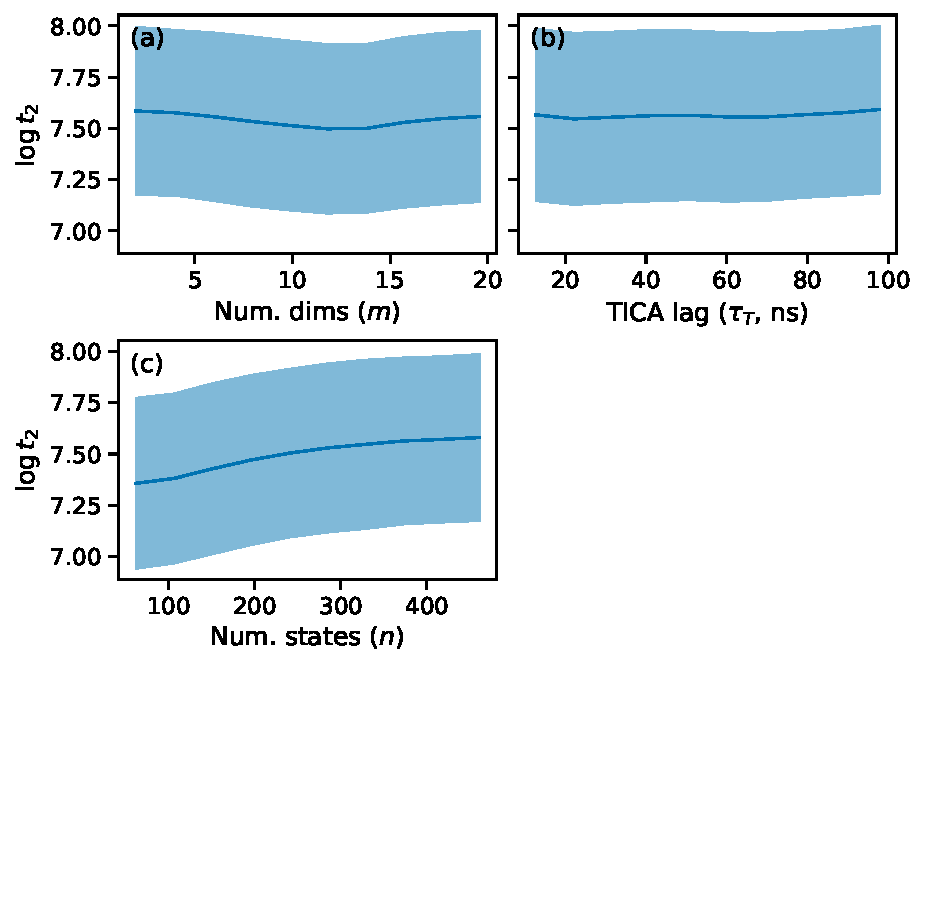
\includegraphics[width=0.8\textwidth, trim={0, 4cm, 0, 0}, clip]{figures/response_surface_marginal_dihedrals_None_ts.pdf}
%     \caption{\textsc{Timescale response surface dihedrals feature}. The solid line is the mean of the Gaussian process and the shaded area is $\pm 2\sigma$. Panel (a) shows the response surface as a function of the number of $m$, the number TICA dimensions. The remaining hyperparameters are fixed at the values at the maximum of the response surface. i.e., $\log{t_2}=f(m, \tau^{*}, n^{*})$ where $m^{*}, \tau^{*}, n^{*} = \argmax \left [f( m, \tau,n)\right]$. Panels (b) and (c) are similar but as functions of the TICA lag time ($
%     \tau_{T}$) and number of microstates ($n$) respectively.}
%     \label{fig:repsonse_diheds}
% \end{figure}

% \begin{figure}
%     \centering
%     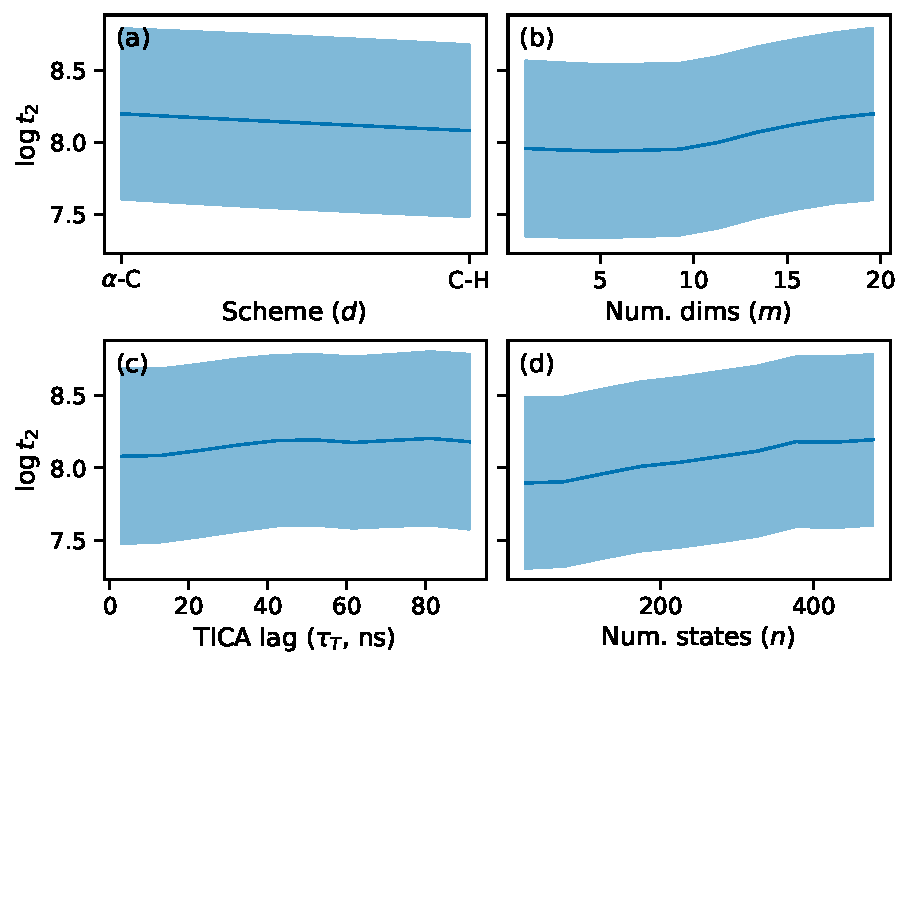
\includegraphics[width=0.8\textwidth, trim={0, 4cm, 0, 0}, clip]{figures/response_surface_marginal_distances_linear_ts.pdf}
    
%     \caption{\textsc{Timescale response surface for distances feature}. The solid line is the mean of the Gaussian process and the shaded area is $\pm 2\sigma$. Panel (a) shows the response surface as a function of the number of $d$, the type of contact distance. The remaining hyperparameters are fixed at the values at the maximum of the response surface. i.e., $\log{t_2}=f(d, m^{*}, \tau^{*}, n^{*})$ where $d^{*}, m^{*}, \tau^{*}, n^{*} = \argmax \left [f(d,  m, \tau,n)\right]$. Panels (b), (c) and (d) are similar but as functions of the number of TICA dimensions ($m$), the TICA lag time ($\tau_{T}$) and number of microstates ($n$) respectively.}
%     \label{fig:repsonse_dist}
% \end{figure}


% \begin{figure}
%     \centering
%     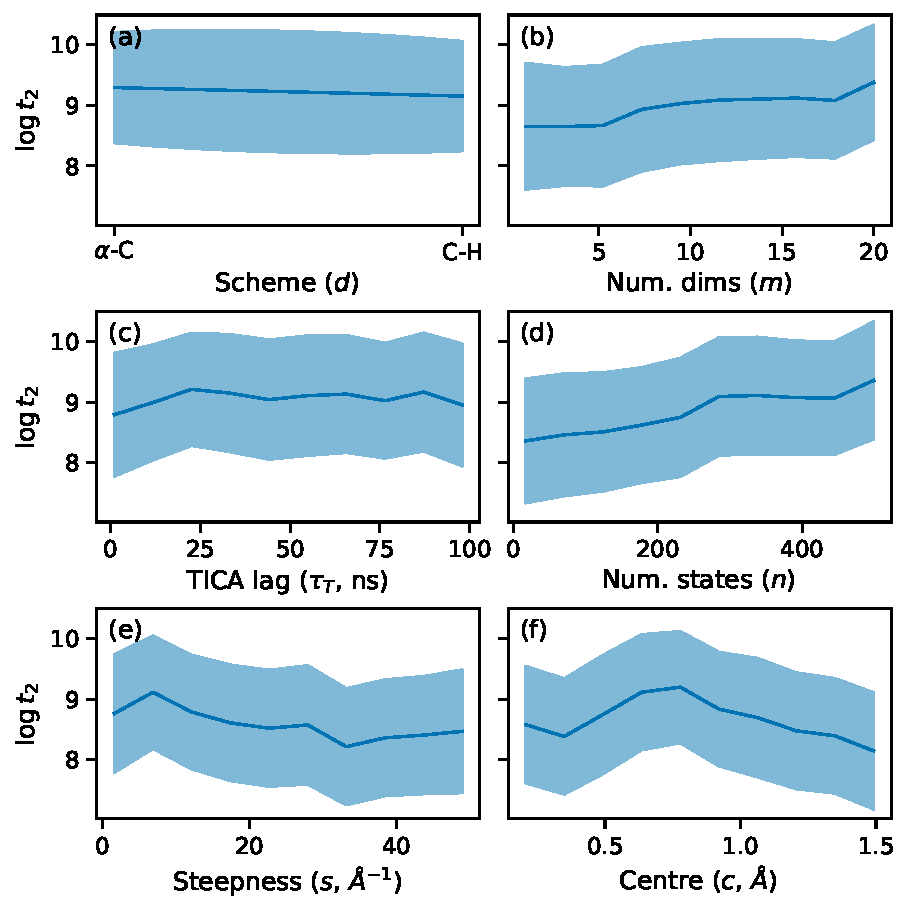
\includegraphics[width=0.8\textwidth]{figures/response_surface_marginal_distances_logistic_ts.pdf}
%     \caption{\textsc{Timescale response surface for logistic distance feature}. The solid line is the mean of the Gaussian process and the shaded area is $\pm 2\sigma$. Panel (a) shows the response surface as a function of the number of $d$, the type of contact distance. The remaining hyperparameters are fixed at the values at the maximum of the response surface. i.e., $\log{t_2}=f(d, m^{*}, \tau^{*}, n^{*}, s^{*}), c^{*})$ where $d^{*}, m^{*}, \tau^{*}, n^{*}, s^{*}, c^{*} = \argmax \left [f(d,  m, \tau,n, s, c)\right]$. Panels (b), (c), (d), (e) and (f) are similar but as functions of the number of TICA dimensions ($m$), the TICA lag time ($\tau_{T}$), number of microstates ($n$), logistic steepness ($s$) and logistic center ($c$) respectively.}
%     \label{fig:repsonse_logistic}
% \end{figure}


% Details on the bootstrapping process


% \section{Bayesian Optimisation}

% \begin{figure}
%     \centering
%     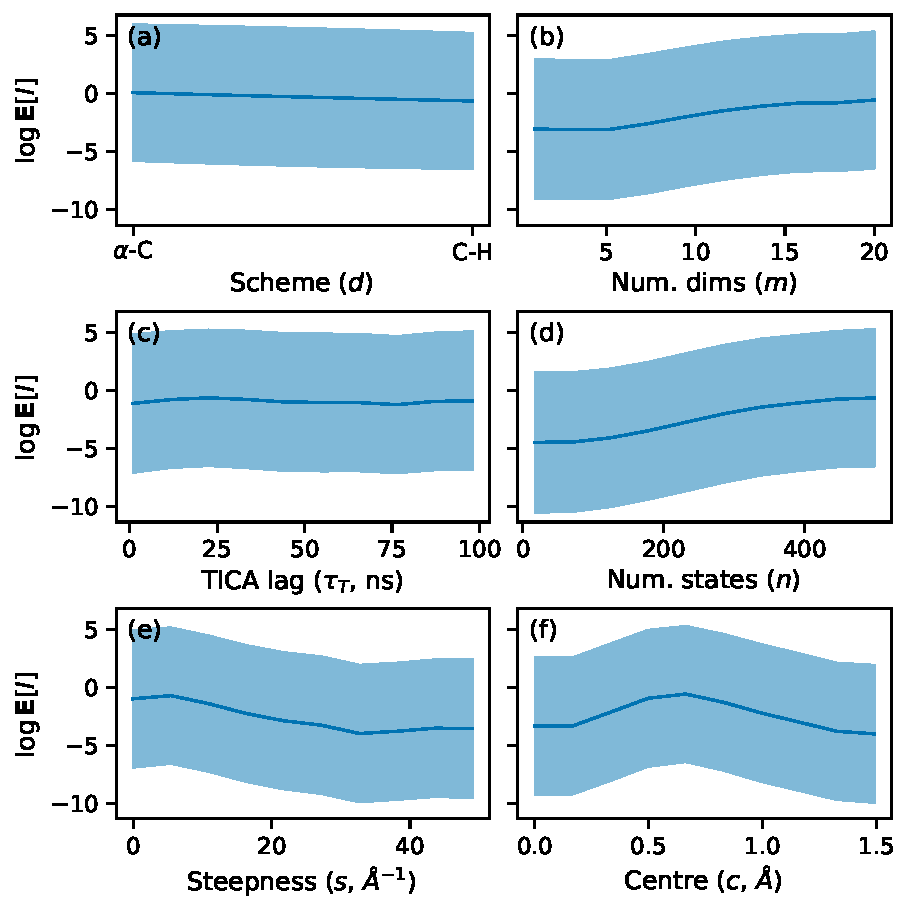
\includegraphics[width=0.8\textwidth]{figures/response_surface_marginal_distances_logistic_ei.pdf}
%     \caption{\textsc{Expected improvement for logistic distance feature}. The solid line is the mean of the Gaussian process and the shaded area is $\pm 2\sigma$. Panel (a) shows the response surface as a function of the number of $d$, the type of contact distance. The remaining hyperparameters are fixed at the values at the maximum of the response surface. i.e., $\log{\mathbb{E}[I]}=f(d, m^{*}, \tau^{*}, n^{*}, s^{*}), c^{*})$ where $d^{*}, m^{*}, \tau^{*}, n^{*}, s^{*}, c^{*} = \argmax \left [f(d,  m, \tau,n, s, c)\right]$. Panels (b), (c), (d), (e) and (f) are similar but as functions of the number of TICA dimensions ($m$), the TICA lag time ($\tau_{T}$), number of microstates ($n$), logistic steepness ($s$) and logistic center ($c$) respectively.}
%     \label{fig:repsonse_ei_logistic}
% \end{figure}

\end{document}
